%definira klasu dokumenta 
\documentclass[12pt]{report} 

%prostor izmedu naredbi \documentclass i \begin{document} se zove uvod. U njemu se nalaze naredbe koje se odnose na cijeli dokument

%osnovni LaTex ne može riješiti sve probleme, pa se koriste različiti paketi koji olakšavaju izradu željenog dokumenta
\usepackage[croatian]{babel} 
\usepackage{amssymb}
\usepackage{amsmath}
\usepackage{txfonts}
\usepackage{mathdots}
\usepackage{titlesec}
\usepackage{array}
\usepackage{lastpage}
\usepackage{etoolbox}
\usepackage{tabularray}
\usepackage{color, colortbl}
\usepackage{adjustbox}
\usepackage{geometry}
\usepackage[classicReIm]{kpfonts}
\usepackage{hyperref}
\usepackage{fancyhdr}

\usepackage{float}
\usepackage{setspace}
\restylefloat{table}


\patchcmd{\chapter}{\thispagestyle{plain}}{\thispagestyle{fancy}}{}{} %redefiniranje stila stranice u paketu fancyhdr

%oblik naslova poglavlja
\titleformat{\chapter}{\normalfont\huge\bfseries}{\thechapter.}{20pt}{\Huge}
\titlespacing{\chapter}{0pt}{0pt}{40pt}


\linespread{1.3} %razmak između redaka

\geometry{a4paper, left=1in, top=1in,}  %oblik stranice

\hypersetup{ colorlinks, citecolor=black, filecolor=black, linkcolor=black,	urlcolor=black }   %izgled poveznice


%prored smanjen između redaka u nabrajanjima i popisima
\newenvironment{packed_enum}{
	\begin{enumerate}
		\setlength{\itemsep}{0pt}
		\setlength{\parskip}{0pt}
		\setlength{\parsep}{0pt}
	}{\end{enumerate}}

\newenvironment{packed_item}{
	\begin{itemize}
		\setlength{\itemsep}{0pt}
		\setlength{\parskip}{0pt}
		\setlength{\parsep}{0pt}
	}{\end{itemize}}




%boja za privatni i udaljeni kljuc u tablicama
\definecolor{LightBlue}{rgb}{0.9,0.9,1}
\definecolor{LightGreen}{rgb}{0.9,1,0.9}

%Promjena teksta za dugačke tablice
\DefTblrTemplate{contfoot-text}{normal}{Nastavljeno na idućoj stranici}
\SetTblrTemplate{contfoot-text}{normal}
\DefTblrTemplate{conthead-text}{normal}{(Nastavljeno)}
\SetTblrTemplate{conthead-text}{normal}
\DefTblrTemplate{middlehead,lasthead}{normal}{Nastavljeno od prethodne stranice}
\SetTblrTemplate{middlehead,lasthead}{normal}

%podesavanje zaglavlja i podnožja

\pagestyle{fancy}
\lhead{Programsko inženjerstvo}
\rhead{Ples}
\lfoot{SBT}
\cfoot{stranica \thepage/\pageref{LastPage}}
\rfoot{\today}
\renewcommand{\headrulewidth}{0.2pt}
\renewcommand{\footrulewidth}{0.2pt}


\begin{document} 
	
	
	
	\begin{titlepage}
		\begin{center}
			\vspace*{\stretch{1.0}} %u kombinaciji s ostalim \vspace naredbama definira razmak između redaka teksta
			\LARGE Programsko inženjerstvo\\
			\large Ak. god. 2022./2023.\\
			
			\vspace*{\stretch{3.0}}
			
			\huge Sreletovi Plesnjaci\\
			\Large Dokumentacija, Rev. \textit{1}\\
			
			\vspace*{\stretch{12.0}}
			\normalsize
			Grupa: \textit{SBT}\\
			Voditelj: \textit{Marko Brlek}\\
			
			
			\vspace*{\stretch{1.0}}
			Datum predaje: \textit{18. 11. 2022.}\\
	
			\vspace*{\stretch{4.0}}
			
			Nastavnik: \textit{Hrvoje Nuić}\\
		
		\end{center}

	
	\end{titlepage}

	
	\tableofcontents


	\chapter{Dnevnik promjena dokumentacije}

		\begin{longtblr}[
				label=none
			]{
				width = \textwidth, 
				colspec={|X[2]|X[13]|X[3]|X[3]|}, 
				rowhead = 1
			}
			\hline
			\textbf{Rev.}	& \textbf{Opis promjene/dodatka} & \textbf{Autori} & \textbf{Datum}\\[3pt] \hline
			0.1 & Napravljen predložak.	& Marko Brlek & 24.10.2022. 		\\[3pt] \hline 
			0.2 & Napisani funkcionalni zahtjevi.	& Filip Šiktar, Martin Čukić& 25.10.2022. 		\\[3pt] \hline
			0.3 & Napisan opis projektnog zadatka	& Viktoria Kežman, Andrej Cirkveni & 25.10.2022. \\[3pt] \hline
			0.4 & Napisani obrasci uporabe, nacrtani dijagrami obrazaca uporabe & Karlo Žižić, Josip Gegač & 26.10.2022. \\[3pt] \hline
			0.5 & Napravljen model i relacijska shema baze podataka & Marko Brlek, Filip Šiktar & 3.11.2022. \\[3pt] \hline
			0.6 & Napisani opisi svih sekvencijskih dijagrama & Viktoria Kežman, Andrej Cirkveni & 5.11.2022. \\[3pt] \hline
			0.7 & Napisan opis arhitekture i baze, nacrtan i opisan dijagram razreda & Viktoria Kežman & 14.11.2022. \\[3pt] \hline
			0.8 & Nacrtan i opisan : dijagram stanja, dijagram aktivnosti, dijagram razmještaja, dijagram komponenti  & Viktoria Kežman & 3.1.2023. \\[3pt] \hline
			0.9 & Dodan odjeljak "korištene tehnologije i alati", dopisana literatura i zaključak  & Viktoria Kežman & 4.1.2023. \\[3pt] \hline
			
			
		\end{longtblr}
	
	
	\chapter{Opis projektnog zadatka „PLESNJACI“ }
\section{Uvod}
		
		Cilj ovog projektnog zadatka je razviti programsku podršku za izradu web aplikacije koja će olakšati pronalaženje i organizaciju plesnih tečajeva i plesnjaka. U nastavku se opisuju najopćenitije stranice web-aplikacije i njihove funkcionalnosti. 
		
\section{Opis funkcionalnosti web aplikacije}
		 
		      Gradimo jednostavnu CRUD aplikaciju, u nastavku navodimo njene osnovne cjeline i prikaz funkcionalnosti.
		 
	 	\subsection{"Početna stranica"}
	
			Prilikom pokretanja web-aplikacije prikazuje se „Početna stranica“. Ako korisnik nije       registriran na početnoj stranici se prikazuju profili klubova i tipovi plesa koje taj klub nudi. Također na stranici se nalazi karta s dostupnim plesnjacima i lokacijama klubova. Neregistriranom korisniku je omogućeno kreiranje računa (registracija) . 
		

			 
			\subsubsection{Karta}
				
			Na karti se mogu filtrirati plesnjaci i klubovi. Plesnjaci se mogu filtrirati po tipu plesa, klubu koji ga organizira i tipovima plesa. Klubovi se mogu filtrirati po tipovima plesa za koje organiziraju tečajeve.
			\bigskip
			\bigskip
			\bigskip
			\bigskip
			\bigskip
			
			
				
			\subsubsection{Registracija}
				
			Ako se korisnik odluči registrirati otvara se odgovarajući obrazac za registraciju koji od njega zahtijeva da upiše sljedeće informacije :
				
				\begin{packed_item}
					\item Korisničko ime
					\item Lozinka
					\item Ime
					\item Prezime
					\item Spol
					\item Datum rođenja
					\item Broj mobitela
					\item Email adresa
					\item Opis plesnog iskustva i fotografija (opcionalno)
				\end{packed_item}
			\bigskip
			
	
  	\subsection {"Stranica u kojoj je korisnik registriran"}
  	Kad se korisnik registrirao on ima ulogu klijenta. Klijent može dodatno stvoriti klub. Ako klijent odluči stvoriti novi klub otvara se odgovarajući obrazac koji zahtijeva sljedeće informacije za taj klub :
		
		
		\begin{packed_item}
			\item Korisničko ime
			\item Lozinka
			\item Ime kluba
			\item Adresa sjedišta
			\item Datum rođenja
			\item Telefon
			\item Email adresa
		\end{packed_item}
	
	Novo registrirani klubovi prvo moraju biti potvrđeni od strane administratora. Ako je korisnik uspio registrirati svoj klub on postaje vlasnikom kluba. Osim uloge klijenta i vlasnika kluba postoji i uloga administratora sustava.
	
	\bigskip
	\bigskip
	\bigskip
	\bigskip
	\bigskip
	\bigskip
	\bigskip
	
		
		
		
		\subsubsection{Registrirani korisnik (klijent)}
	
			
		Klijent može pregledati, mijenjati osobne podatke i izbrisati svoj korisnički račun. Također na karti mu je omogućeno prikazivanje tečajeva koji su slobodni za upis, a rezultate može filtrirati po željenom vremenu i tipu plesa. 
		Odabirom tečaja, otvaraju se relevantne informacije poput vrste plesa, kalendar te ime, prezime i slika trenera. Kalendar ima zapisane termine tečaja i lokacije s dvoranom za svaki termin.
		

			
			\subsubsection{Registrirani korisnik(vlasnik kluba)}
			Vlasnik kluba je zadužen za organizaciju plesnjaka koji se mogu izvoditi i na lokacijama izvan prostorija kluba, a sadrže naziv, opis i sliku. Na plesnjaku se mogu plesati različiti tipovi plesa. Svaki klub ima svoju naslovnu stranicu (profil) i popis trenera.
			Svaki trener ima podstranicu na kojima ima popis grupa koje trenira, a svi termini tečaja koje vodi su mu prikazani na kalendaru. Trener prilikom otvaranja tečaja za kojeg je zadužen uz opće informacije dobiva popis klijenata koji bi trebali biti nazočni.
			Na profilu kluba su prikazane informacije o :
			
			
			
			\begin{packed_item}
				\item imenu kluba
				\item kontakt telefon
				\item email adresa
				\item kratki opis
				\item poveznica na stranicu s grupama za upis
				\item popis plesova koje njihovi treneri mogu voditi
				\item prikaz lokacija na karti
				\item popis dvorana po lokacijama
			\end{packed_item}
		
		Vlasnik kluba na naslovnoj stranici kluba može objaviti upise za tečaj s krajnjim rokom prijave. Upisi u grupu mogu biti ograničavajući ovisno o dobi i spolu. Grupi je dodijeljen trener iz kluba, skup treninga kroz neko vrijeme, maksimalni broj sudionika te opis u kojem pišu dodatne informacije o težini treninga, posebnim uvjetima treniranja, pravila ponašanja i slično.
		
			\bigskip
			\bigskip
			\bigskip
			\bigskip
			\bigskip
			
			\subsubsection{Poveznica klijenta i klijenta kao vlasnika kluba}
			
		Bilo koji klijent može vlasniku kluba poslati prijavu da postane trener, a vlasnik kluba ga potom može  potvrditi. Prijava sadrži:
		
			\begin{packed_item}
				\item motivacijsko pismo
				\item potvrda da je klijent osposobljen držati tečaj plesa (pdf dokument)
			\end{packed_item}
		Klijent može pregledati aktivne prijave na tečaj od kluba i prijaviti se. Nakon isteka roka upisa, vlasnik kluba treba odabrati klijente koji se primaju u grupu. Vlasnik kluba može naknadno mijenjati popis klijenata, uređivati i brisati grupe.
		
			\bigskip
			
			\subsubsection{Administrator}
			
			Administrator može dodati, mijenjati i brisati plesove. Odobrava novo registrirane klubove kako bi postali valjani. Također može pregledati popis svih klijenata i klubova te uređivati korisničke račune.
			Plesovi sadrže:
			\begin{packed_item}
				\item naziv
				\item kratki opis
				\item sliku
				\item link na video primjer tog plesa
			\end{packed_item}
	\chapter{Specifikacija programske potpore}
		
	\section{Funkcionalni zahtjevi}
	\bigskip
		
			\noindent \textbf{Dionici:}
			
			\begin{packed_enum}
				
				\item Klijent
				\item Klub
				\item Trener
				\item Administrator
				\item Razvojni tim
				
			\end{packed_enum}
		\bigskip
		\bigskip
	
		
			
			\noindent \textbf{Aktori i njihovi funkcionalni zahtjevi:}
			\bigskip
		
			\begin{packed_enum}
				\item  \underbar{Neregistrirani/neprijavljeni korisnik (inicijator) može:}
				
				\begin{packed_enum}
					
					\item pregledati profil kluba i tipove plesova koje klub nudi
					\item pregledati karte dostupnih plesnjaka i lokacije klubova
					\item filtrirati plesnjake po:
					\begin{packed_enum}
						
						\item  tipu plesa
						\item  klubu organizatoru i tipu plesa
				
					\end{packed_enum}
					\item  filtrirati klubove po tipovima plesa za koje organiziraju tečaj
					\item kreirati račun (korisničko ime, lozinka, prezime, spol, datum rođenja, broj mobitela, email adresa, opcionalno opis plesnog iskustva i fotografija)
						
				\end{packed_enum}
			\bigskip
			\bigskip
			\bigskip
			\bigskip
			\bigskip
			\bigskip
			\bigskip
			\bigskip
			\bigskip
			

				\item \underbar{Klijent (inicijator) može:}
				
				\begin{packed_enum}
					\item pregledati i izmijeniti osobne podatke
					\item obrisati korisnički račun
					\item prikazati tečajeve slobodne za upis, na karti:
					\begin{packed_enum}
						\item rezultate filtrirati po vremenu održavanja i tipu plesa
					\end{packed_enum}
					\item odabrati tečaj (vrsta plesa, kalendar održavanja, ime i prezime te slika trenera)
					\item klubu poslati prijavu da postane trener:
					\begin{packed_enum}
						\item postavi motivacijsko pismo
						\item postavi pdf datoteku potvrde da je sposoban držati tečaj
					\end{packed_enum}
					\item pregledati aktivne prijave na tečaj nekog kluba
					\item prijaviti se na tečaj kluba
					\item poslati zahtjev za otvaranje kluba
				\end{packed_enum}
			\bigskip
			\bigskip
				
				\item \underbar{Administrator (inicijator) može:}
				\begin{packed_enum}
					\item potvrditi nove registrirane klubove
					\item dodavati, mijenjati i brisati plesove
					\item pregledati popise svih klijenata i klubova
					\item uređivati korisničke račune
				\end{packed_enum}
			\bigskip
			\bigskip
				
				\item \underbar{Vlasnik kluba (inicijator) može:}
				\begin{packed_enum}	
					\item raditi sve isto kao i klijent
					\item pregledati i izmijeniti osobne podatke kluba 
					\item obrisati korisnički račun kluba 
					\item organizirati plesnjak (lokacija, naziv, opis i slika, tipovi plesa)
					\item potvrditi klijentovu prijavu za trenera
					\item prikazati informacije:
					\begin{packed_enum}
						\item ime kluba, kontakt telefon, email adresa, kratki opis kluba
						\item popis plesova koje njihovi treneri izvode
						\item prikaz lokacija plesova i dvorana na karti
					\end{packed_enum}
					\item postaviti poveznicu na stranicu s grupama za upis
					\item objaviti upis za tečaj s vremenskim rokom
					\item odabrati klijente koji se primaju u grupu
					\item mijenjati popis klijenata
					\item urediti ili brisati grupe
				\end{packed_enum}
			\bigskip
			\bigskip
				
				\item \underbar{Baza podataka (sudionik) može:}
				\begin{packed_enum}
					\item pohraniti podatke o korisnicima i njihovim ovlasitima
					\item pohraniti podatke o klubovima, plesovima koje oni nude, tečajevima, dvoranama i lokacijama odvijanja
				\end{packed_enum}
			\bigskip
			\bigskip
				
				\item \underbar{Trener (inicijator) može:}
				\begin{packed_enum}
					\item raditi sve isto kao i klijent
					\item pregledati popis grupa koje trenira
					\item pregledati termine tečajeva koje vodi na kalendaru
					\item pregledati popise klijenata koji bi trebali biti nazočni
				\end{packed_enum}
					
				%\item  \underbar{Grupa (inicijator) može:}
				
			%	\begin{packed_enum}
					
				%	\item pregledati podatke o treneru
				%	\item pregledati skup treninga kroz neki vremenski period
				%	\item pregledati maksimalan broj sudionika
				%	\item dati informaciju o težini treninga
				%	\item postaviti uvjete treniranja, pravila ponašanja
					
				%\end{packed_enum}
			\end{packed_enum}
			
			\eject 
			
			
				
			\subsection{Obrasci uporabe}
				

				\subsubsection{Opis obrazaca uporabe}
					\textit{ Obrasci uporabe (Use Cases) numerirani su oznakama od UC1 do UC32, pomoću njih opisujemo tipičnu uporabu sustava.}\\
				
					\noindent \underbar{\textbf{UC1 - Pregled klubova}}
					\begin{packed_item}
						
						\item \textbf{Glavni sudionik: Neregistrirani korisnik, klijent}
						\item  \textbf{Cilj: Pregled klubova} 
						\item  \textbf{Sudionici: Baza podataka}
						\item  \textbf{Preduvjet: -}
						\item  \textbf{Opis osnovnog tijeka: }
						
						\item[] \begin{packed_enum}
							
							\item Karta je prikazana prilikom učitavanja aplikacije
							\item Neregistrirani korisnik/klijent na karti vidi lokacije klubova te odabire klub
							\item Prikazuju se informacije o klubu, tečajevima te plesnjacima
							
						\end{packed_enum}
				\end{packed_item}
			
					\noindent \underbar{\textbf{UC2 - Registracija korisnika}}
					\begin{packed_item}
						
						\item \textbf{Glavni sudionik: Neregistrirani korisnik}
						\item  \textbf{Cilj: Stvoriti korisnički račun za pristup sustavu} 
						\item  \textbf{Sudionici: Baza podataka}
						\item  \textbf{Preduvjet: -}
						\item  \textbf{Opis osnovnog tijeka: }
						
						\item[] \begin{packed_enum}
							
							\item Neregstrirani korisnik odabire opciju za registraciju
							\item Neregistrirani korisnik unosi sve potrebne informacije kako bi se registrirao
							\item Klijentu se prikazuju informacije početne stranice
							
						\end{packed_enum}
						
						\item  \textbf{Opis mogućih odstupanja:}
						
						\item[] \begin{packed_item}
							
							\item[2.a] Unos podataka u neispravnom formatu, email ili korisničko ime koje je već korišteno od strane drugog klijenta, email ili korisničko ime koje nije registrirano
							\item[] \begin{packed_enum}
								
								\item Sustav obaviještava neregistriranog korisnika o grešci te ga vraća opet na stranicu za registraciju
								\item Neregistrirani korisnik unosi ispravne podatke te se uspješno registrira ili odustaje od registracije
								
							\end{packed_enum}
							
							
							
						\end{packed_item}
						
					\end{packed_item}
				
					\noindent \underbar{\textbf{UC3 - Prijava u sustav}}
					\begin{packed_item}
						
						\item \textbf{Glavni sudionik: Klijent}
						\item  \textbf{Cilj: Dobiti pristup korisničkom sučelju} 
						\item  \textbf{Sudionici: Baza podataka}
						\item  \textbf{Preduvjet: prethodna registracija}
						\item  \textbf{Opis osnovnog tijeka: }
						
						\item[] \begin{packed_enum}
							
							\item Unos korisničkog imena i lozinke
							\item Potvrda o ispravnosti unesenih podataka
							\item Pristup klijentskim funkcijama
							
						\end{packed_enum}
						
						\item  \textbf{Opis mogućih odstupanja:}
						
						\item[] \begin{packed_item}
							
							\item[2.a] Neispravno uneseno korisničko ime ili lozinka
							\item[] \begin{packed_enum}
								
								\item Sustav obaviještava klijenta te ga vraća na stranicu za prijavu
								
							\end{packed_enum}
							
						\end{packed_item}
						
					\end{packed_item}
				
					\noindent \underbar{\textbf{UC4 - Pregled osobnih podataka}}
					\begin{packed_item}
						
						\item \textbf{Glavni sudionik: Klijent}
						\item  \textbf{Cilj: Pregledati osobne podatke} 	
						\item  \textbf{Sudionici: Baza podataka}
						\item  \textbf{Preduvjet: Klijent je prijavljen u sustav}
						\item  \textbf{Opis osnovnog tijeka: }
						
						\item[] \begin{packed_enum}
							
							\item Klijent odabire opciju "Osobni podatci"
							\item Aplikacija prikazuje osobne podatke klijenta
						\end{packed_enum}
					
				\end{packed_item}
						
					\noindent \underbar{\textbf{UC5 - Promjena osobnih podataka}}
					\begin{packed_item}
							
						\item \textbf{Glavni sudionik: Klijent}
						\item  \textbf{Cilj: Promijeniti osobne podatke} 
						\item  \textbf{Sudionici: Baza podataka}
						\item  \textbf{Preduvjet: Klijent je prijavljen u sustav}
						\item  \textbf{Opis osnovnog tijeka: }
							
						\item[] \begin{packed_enum}
								
							\item Klijent odabire opciju za promjenu osobnih podataka
							\item Klijent unosi nove podatke te ih sprema
							\item Baza podataka se ažurira
						\end{packed_enum}
							
						\item  \textbf{Opis mogućih odstupanja:}
							
						\item[] \begin{packed_item}
								
							\item[2.a] Klijent unosi nove podatke, ali ih ne sprema
							\item[] \begin{packed_enum}
									
								\item Aplikacija obaviještava klijenta da mora spremiti promijenjene podatke
									
							\end{packed_enum}
								
						\end{packed_item}
							
					\end{packed_item}
					
					\noindent \underbar{\textbf{UC6 - Brisanje korisničkog računa}}
					\begin{packed_item}
						
						\item \textbf{Glavni sudionik: Klijent}
						\item  \textbf{Cilj: Izbrisati svoj korisnički račun} 
						\item  \textbf{Sudionici: Baza podataka}
						\item  \textbf{Preduvjet: Klijent je prijavljen u sustav}
						\item  \textbf{Opis osnovnog tijeka: }
						
						\item[] \begin{packed_enum}
							
							\item Klijent pregledava osobne podatke
							\item Otvara se stranica sa osobnim podatcima klijenta
							\item Klijent briše korisnički račun
							\item Korisnički račun se briše iz baze podataka
							\item Otvara se početna stranica
						\end{packed_enum}
						
						
					\end{packed_item}
				\bigskip
					\bigskip
						\bigskip
					
						\noindent \underbar{\textbf{UC7 - Prikaz  tečajeva}}
						\begin{packed_item}
							
							\item \textbf{Glavni sudionik: Klijent}
							\item  \textbf{Cilj: Prikazati tečajeve slobodne za upis na karti} 
							\item  \textbf{Sudionici: Baza podataka}
							\item  \textbf{Preduvjet: Klijent je prijavljen u sustav }
							\item  \textbf{Opis osnovnog tijeka: }
							
							\item[] \begin{packed_enum}
								
								\item Klijentu se na karti prikazuje popis  tečajeva
							\end{packed_enum}
							\bigskip
								\bigskip
									\bigskip
							
							
						\end{packed_item}
					
						\noindent \underbar{\textbf{UC8 - Pregled profila kluba}}
						\begin{packed_item}
							
							\item \textbf{Glavni sudionik: Klijent}
							\item  \textbf{Cilj: Pregledati podatke o klubu} 
							\item  \textbf{Sudionici: Baza podataka}
							\item  \textbf{Preduvjet: Klijent je prijavljen u sustav}
							\item  \textbf{Opis osnovnog tijeka: }
							
							\item[] \begin{packed_enum}
								
								\item Klijent na početnoj stranici na karti odabire klub
								\item Klijentu se prikazuje stranica kluba
							\end{packed_enum}
							
						\end{packed_item}
						\bigskip
							\bigskip
								\bigskip
									\bigskip
										\bigskip
											\bigskip
												\bigskip
													\bigskip
														\bigskip
															\bigskip
																\bigskip
																	\bigskip
																		\bigskip
					
						\noindent \underbar{\textbf{UC9 - Prijava za trenera}}
						\begin{packed_item}
							
							\item \textbf{Glavni sudionik: Klijent}
							\item  \textbf{Cilj: Postati trener} 
							\item  \textbf{Sudionici: Baza podataka}
							\item  \textbf{Preduvjet: Klijent je prijavljen u sustav}
							\item  \textbf{Opis osnovnog tijeka: }
							
							\item[] \begin{packed_enum}
								
								\item Klijent na stranici kluba odabire opciju "Prijava za trenera"
								\item Klijent dodaje potrebne dokumente
								\item Klijent čeka odobrenje vlasnika kluba

							\end{packed_enum}
							\bigskip
								\bigskip

							
						\end{packed_item}
						
						\noindent \underbar{\textbf{UC10 - Odobravanje klijenta za trenera}}
						\begin{packed_item}
							
							\item \textbf{Glavni sudionik: Vlasnik kluba}
							\item  \textbf{Cilj: Prihvatiti ili odbiti prijavu klijenta za trenera u klubu} 
							\item  \textbf{Sudionici: Baza podataka, Klijent}
							\item  \textbf{Preduvjet: Poslana je prijava za trenera, klijent je vlasnik kluba}
							\item  \textbf{Opis osnovnog tijeka: }
							
							\item[] \begin{packed_enum}
								
								\item Vlasnik kluba odabire opciju "Aktivne prijave za trenera"
								\item Prikazuju se aktivne prijave za trenera
								\item Vlasnik kluba potvrđuje ili odbija prijave

							\end{packed_enum}
							\bigskip
								\bigskip
							
						\end{packed_item}
					
						\noindent \underbar{\textbf{UC11 - Stvaranje klubova}}
						\begin{packed_item}
							
							\item \textbf{Glavni sudionik: Klijent}
							\item  \textbf{Cilj: Stvoriti novi klub i postati vlasnik kluba} 
							\item  \textbf{Sudionici: Baza podataka}
							\item  \textbf{Preduvjet: Korisnik je prijavljen u sustav}
							\item  \textbf{Opis osnovnog tijeka: }
							
							\item[] \begin{packed_enum}
								
								\item Klijent na profilnoj stranici odabire opciju "Stvori klub"
								\item Klijent unosi sve informacije potrebne za stvaranje kluba
								\item Klijent čeka da administrator potvrdi klub

							\end{packed_enum}
						
							\item  \textbf{Opis mogućih odstupanja:}
							
							\item[] \begin{packed_item}
								
								\item[2.a] Klub s istim imenom već postoji
								\item[] \begin{packed_enum}
									
									\item Sustav obaviještava klijenta da klub s istim imenom već postoji i vraća klijenta na stranicu za stvaranje kluba
									
								\end{packed_enum}
								
								
								
							\end{packed_item}
							
							
						\end{packed_item}
					
						\noindent \underbar{\textbf{UC12 - Brisanje kluba}}
						\begin{packed_item}
							
							\item \textbf{Glavni sudionik: Administrator}
							\item  \textbf{Cilj: Obrisati klub iz sustava} 
							\item  \textbf{Sudionici: Baza podataka}
							\item  \textbf{Preduvjet: Klijent ima dodijeljena prava Administratora}
							\item  \textbf{Opis osnovnog tijeka: }
							
							\item[] \begin{packed_enum}
								
								\item Administrator odabire klub
								\item Administrator odabire opciju "Obriši klub"
								\item Klub se briše sa stranice

							\end{packed_enum}
							\bigskip
								\bigskip
							
						\end{packed_item}
					
						\noindent \underbar{\textbf{UC13- Organizacija plesnjaka}}
						\begin{packed_item}
							
							\item \textbf{Glavni sudionik: Vlasnik kluba}
							\item  \textbf{Cilj: Organizirati plesnjak} 
							\item  \textbf{Sudionici: Baza podataka}
							\item  \textbf{Preduvjet: Klijent je vlasnik kluba}
							\item  \textbf{Opis osnovnog tijeka: }
							
							\item[] \begin{packed_enum}
								
								\item Vlasnik kluba na stranici kluba odabire pregled plesnjaka
								\item Prikazuje se popis plesnjaka
								\item Vlasnik kluba odabire opciju "Dodaj plesnjak"
								\item Vlasnik kluba unosi informacije o plesnjaku
								\item Stvara se novi plesnjak
							\end{packed_enum}
							
						\end{packed_item}
						\bigskip
							\bigskip
					
						\noindent \underbar{\textbf{UC14 - Prikaz tečaja za trenere}}
						\begin{packed_item}
							
							\item \textbf{Glavni sudionik: Trener}
							\item  \textbf{Cilj: Pregledati tečajeve koje trener drži} 
							\item  \textbf{Sudionici: Baza podataka}
							\item  \textbf{Preduvjet: Trener je prijavljen u sustavu te ima dodijeljen klub i tečaj}
							\item  \textbf{Opis osnovnog tijeka: }
							
							\item[] \begin{packed_enum}
								
								\item Trener na profilnoj stranci odabire popis tečajeva koje vodi
								\item Prikazuje se popis tečajeva

							\end{packed_enum}
							
						\end{packed_item}
						\newpage
					
						\noindent \underbar{\textbf{UC15 - Prikaz popisa klijenata koji bi trebali biti nazočni}}
						\begin{packed_item}
							
							\item \textbf{Glavni sudionik: Trener}
							\item  \textbf{Cilj: Prikazati treneru popis klijenata} 
							\item  \textbf{Sudionici: Baza podataka}
							\item  \textbf{Preduvjet: Trener je prijavljen u sustav te mu je dodijeljen klub te barem jedan tečaj}
							\item  \textbf{Opis osnovnog tijeka: }
							
							\item[] \begin{packed_enum}
								
								\item Trener na popisu tečajeva odabire određeni tečaj
								\item Trener odabire opciju "Prikaži sudionike"
								\item Prikazuje se popis klijenata koji su prijavljeni na tečaj

							\end{packed_enum}
							
						\end{packed_item}
						\bigskip
							\bigskip
								\bigskip
					
						\noindent \underbar{\textbf{UC16 - Objava upisa za tečaj}}
						\begin{packed_item}
							
							\item \textbf{Glavni sudionik: Vlasnik kluba}
							\item  \textbf{Cilj: Objaviti upis za tečaj} 
							\item  \textbf{Sudionici: Baza podataka}
							\item  \textbf{Preduvjet: Klub je prijavljen i odobren u sustavu}
							\item  \textbf{Opis osnovnog tijeka: }
							
							\item[] \begin{packed_enum}
								
								\item Vlasnik kluba odabire klub
								\item Vlasniku se prikazuje popis tečajeva odabranog kluba
								\item Vlasnik kluba odabire tečaj
								\item Vlasnik odabire opciju "Objavi upis"
								\item Vlasnik upisuje podatke o grupi
								\item Vlasnik prima obavijet o uspješnoj objavi upisa
							\end{packed_enum}
							
							\item  \textbf{Opis mogućih odstupanja:}
							
							\item[] \begin{packed_item}
								
								\item[2.a] Nisu upisani svi potrebni podaci za grupu ili su neispravno unešeni
								\item[] \begin{packed_enum}
									
									\item Sustav obavjestava korisnika o neuspjelom upisu i vraća ga na stranicu za upisivanje podatka o upisu
									\item Korisnik upisuje ili mijenja potrebne podatke te zavrsava unos ili odustaje od objave upisa
									
								\end{packed_enum}
								
							\end{packed_item}
							
						\end{packed_item}
						\newpage
						
						\noindent \underbar{\textbf{UC17 - Prijava na tečaj}}
						\begin{packed_item}
							
							\item \textbf{Glavni sudionik: Klijent}
							\item  \textbf{Cilj: Prijaviti se na tečaj} 
							\item  \textbf{Sudionici: Baza podataka}
							\item  \textbf{Preduvjet: Klijent je prijavljen u sustav}
							\item  \textbf{Opis osnovnog tijeka: }
							
							\item[] \begin{packed_enum}
								
								\item Klijent odabire tečaj
								\item Klijent odabire opciju "Prijavi se na tečaj"
								\item Prijava se zapisuje u bazu podataka
								\item Klijent dobiva potvrdu o prijavi
							\end{packed_enum}
							
							
							
						\end{packed_item}
						
						\noindent \underbar{\textbf{UC18 - Pregled aktivnih prijava na tečaj od kluba}}
						\begin{packed_item}
							
							\item \textbf{Glavni sudionik: Klijent}
							\item  \textbf{Cilj: Pregledati aktivne prijave na tečaj od kluba} 
							\item  \textbf{Sudionici: Baza podataka}
							\item  \textbf{Preduvjet: Klijent je prijavljen u sustavu}
							\item  \textbf{Opis osnovnog tijeka: }
							
							\item[] \begin{packed_enum}
								
								\item Klijent odabire klub
								\item Klijentu se prikazuje popis tečajeva odabranog kluba
								\item Klijent odabire opciju filtriranja tečajeva kojima su otvorene prijave
								\item Prikažu se sve aktivne prijave tečaja odabranog kluba
							\end{packed_enum}
							
							
							
						\end{packed_item}
						
						\noindent \underbar{\textbf{UC19 - Odabir klijenata koji se primaju na tečaj}}
						\begin{packed_item}
							
							\item \textbf{Glavni sudionik: Vlasnik kluba}
							\item  \textbf{Cilj: Odabrati klijente koji se primaju na tečaj od kluba} 
							\item  \textbf{Sudionici: Baza podataka}
							\item  \textbf{Preduvjet: Klub je prijavljen u sustav i odobren u sustavu te postoje klijenti prijavljeni za tečaj}
							\item  \textbf{Opis osnovnog tijeka: }
							
							\item[] \begin{packed_enum}
								
								\item Vlasnik kluba odabire tečaj
								\item Vlasnik kluba odabire opciju "Pregledaj prijave"
								\item Vlasniku kluba se otvaraju sve molbe za prijavu.
								\item Vlasnik kluba odabire opciju primanja klijenta
								\item Popis primljenih klijenta se pohranjuju u bazu
							\end{packed_enum}
							
							
							
						\end{packed_item}
					\newpage
						
						\noindent \underbar{\textbf{UC20 - Dodavanje klijenata}}
						\begin{packed_item}
							
							\item \textbf{Glavni sudionik: Vlasnik kluba}
							\item  \textbf{Cilj: Dodati klijenta na tečaj} 
							\item  \textbf{Sudionici: Baza podataka}
							\item  \textbf{Preduvjet: Klub je prijavljen i odobren u sustavu}
							\item  \textbf{Opis osnovnog tijeka: }
							
							\item[] \begin{packed_enum}
								
								\item Vlasnik kluba odabire tečaj
								\item Vlasnik kluba odabire opciju "Pregledaj klijente"
								\item Vlasniku kluba se otvaraju sve klijenti odabranog tečaja.
								\item Vlasnik odabire opciju "dodavanje klijenta"
								\item Vlasnik unosi podatke o klijentu
								\item Promjene se upisuju u bazu podataka
							\end{packed_enum}
							
							\item  \textbf{Opis mogućih odstupanja:}
							
							\item[] \begin{packed_item}
								
								\item[2.a] Ne postoji klijent sa danim podatcima
								\item[] \begin{packed_enum}
									
									\item Sustav obavjestava korisnika o neuspjelom upisu i vraća ga na stranicu za dodavanje klijenta
									\item Korisnik mijenja potrebne podatke te zavrsava unos ili odustaje od dodavanja klijenta
									
								\end{packed_enum}
								
							\end{packed_item}
							
						\end{packed_item}
							\bigskip
								\bigskip
						\noindent \underbar{\textbf{UC21 - Brisanje klijenata}}
						\begin{packed_item}
							
							\item \textbf{Glavni sudionik: Vlasnik Kluba}
							\item  \textbf{Cilj: Obrisati klijenta sa popisa} 
							\item  \textbf{Sudionici: Baza podataka}
							\item  \textbf{Preduvjet: Klub je prijavljen i odobren u sustavu te postoje klijenti na popisu}
							\item  \textbf{Opis osnovnog tijeka: }
							
							\item[] \begin{packed_enum}
								
								\item Vlasnik kluba odabire tečaj
								\item Vlasnik kluba odabire opciju "Pregledaj klijente"
								\item Vlasniku kluba se otvaraju sve klijenti odabranog tečaja.
								\item Vlasnik odabire opciju brisanja klijenta
								\item Nakon uredivanja potvrduje izmjenu
								\item Promjene se upisuju u bazu podataka
							\end{packed_enum}
							
							
							
						\end{packed_item}
					\newpage
						
						\noindent \underbar{\textbf{UC22 - Brisanje tečajeva}}
						\begin{packed_item}
							
							\item \textbf{Glavni sudionik: Vlasnik kluba}
							\item  \textbf{Cilj: Obrisati tečaj} 
							\item  \textbf{Sudionici: Baza podataka}
							\item  \textbf{Preduvjet: Klub je prijavljen i odobren u sustavu}
							\item  \textbf{Opis osnovnog tijeka: }
							
							\item[] \begin{packed_enum}
								
								\item Vlasnik kluba odabire klub
								\item Vlasniku se prikazuje popis tečajeva odabranog kluba
								\item Vlasnik briše tečaj odabranog kluba
							\end{packed_enum}
							
							
							
						\end{packed_item}
					
						\noindent \underbar{\textbf{UC23 - Uređivanje tečajeva}}
						\begin{packed_item}
							
							\item \textbf{Glavni sudionik: Vlasnik kluba}
							\item  \textbf{Cilj: Urediti podatke o tečaju} 
							\item  \textbf{Sudionici: Baza podataka}
							\item  \textbf{Preduvjet: Klijent je vlasnik kluba}
							\item  \textbf{Opis osnovnog tijeka: }
							
							\item[] \begin{packed_enum}
								
								\item Vlasnik kluba odabire tečaj
								 \item Vlasniku se prikazuju informacije o tečaju
								\item Vlasnik kluba uređuje atribute tečaja
								\item Vlasnik sprema promjene tečaja
							\end{packed_enum}
							
							\item  \textbf{Opis mogućih odstupanja:}
							
							\item[] \begin{packed_item}
								
								\item[3.a] Vlasnik radi nedozvoljene promjene atributa
								\item[] \begin{packed_enum}
									
									\item Baza ga upozorava da ove promjene nisu dozvoljene
									\item Vlasnik korigira unešene informacije
									
								\end{packed_enum}
							
							\end{packed_item}
							
						\end{packed_item}
						
						\noindent \underbar{\textbf{UC24 - Dodavanje plesa}}
						\begin{packed_item}
							
							\item \textbf{Glavni sudionik: Administrator}
							\item  \textbf{Cilj: Dodati ples} 
							\item  \textbf{Sudionici: Baza podataka}
							\item  \textbf{Preduvjet: Klijent je prijavljen u sustav sa administratorskim pravima}
							\item  \textbf{Opis osnovnog tijeka: }
							
							\item[] \begin{packed_enum}
								
								\item Administrator odabire prikaz svih plesova
								\item Administrator odabire dodavanje novog plesa
								\item Unose se potrebne informacije za ples
								\item Administrator sprema promjene
							\end{packed_enum}
							
							\item  \textbf{Opis mogućih odstupanja:}
							
							\item[] \begin{packed_item}
								
								\item[3.a] Nisu unesene adekvatne informacije o plesu
								\item[] \begin{packed_enum}
									
									\item Baza upozorava na nepravilno dodavanje plesa
									\item Administrator korigira unešene informacije
									
								\end{packed_enum}
								
							\end{packed_item}
							
						\end{packed_item}
						\bigskip
							\bigskip
					
						\noindent \underbar{\textbf{UC25 - Uređivanje plesa}}
						\begin{packed_item}
							
							\item \textbf{Glavni sudionik: Administrator}
							\item  \textbf{Cilj: Urediti podatke o plesu} 
							\item  \textbf{Sudionici: Baza podataka}
							\item  \textbf{Preduvjet: Klijent je prijavljen u sustav sa administratorskim pravima te postoji ples}
							\item  \textbf{Opis osnovnog tijeka: }
							
							\item[] \begin{packed_enum}
								
								\item Administrator odabire ples
								\item Administratoru se prikazuju informacije o plesu
								\item Administrator uređuje željene atribute
								\item Spremaju se promjene
							\end{packed_enum}
							
							\item  \textbf{Opis mogućih odstupanja:}
							
							\item[] \begin{packed_item}
								
								\item[3.a] Administrator radi nedozvoljene promjene atributa
								\item[] \begin{packed_enum}
									
									\item Baza upozorava na nedozvoljene promjene atributa
									\item Administrator korigira unešene informacije
									
								\end{packed_enum}
							
							\end{packed_item}
							
						\end{packed_item}
						\bigskip
							\bigskip
					
						\noindent \underbar{\textbf{UC26 - Brisanje plesa}}
						\begin{packed_item}
							
							\item \textbf{Glavni sudionik: Administrator}
							\item  \textbf{Cilj: Obrisati ples} 
							\item  \textbf{Sudionici: Baza podataka}
							\item  \textbf{Preduvjet: Klijent je prijavljen u sustav sa administratorskim pravima te postoji ples}
							\item  \textbf{Opis osnovnog tijeka: }
							
							\item[] \begin{packed_enum}
								
								\item Administrator odabire prikaz svih plesova
								\item Administrator odabire plesove koje želi obrisati
								\item Administrator sprema promjene
							\end{packed_enum}
							
						\end{packed_item}
					\newpage
					
						\noindent \underbar{\textbf{UC27 - Pregled popisa svih klijenata}}
						\begin{packed_item}
							
							\item \textbf{Glavni sudionik: Administrator}
							\item  \textbf{Cilj: Pregledati popis svih klijenata} 
							\item  \textbf{Sudionici: Baza podataka}
							\item  \textbf{Preduvjet: Klijent je prijavljen u sustav sa administratorskim pravima te postoje klijenti}
							\item  \textbf{Opis osnovnog tijeka: }
							
							\item[] \begin{packed_enum}
								
								\item Administrator odabire popis klijenata
								\item Prikazuje se popis svih klijenata
							\end{packed_enum}
							
						\end{packed_item}
						\bigskip
							\bigskip
					
						\noindent \underbar{\textbf{UC28 - Brisanje klijenata}}
						\begin{packed_item}
							
							\item \textbf{Glavni sudionik: Administrator}
							\item  \textbf{Cilj: Obrisati klijenta} 
							\item  \textbf{Sudionici: Baza podataka}
							\item  \textbf{Preduvjet: Klijent je prijavljen u sustav sa administratorskim pravima te postoji klijent}
							\item  \textbf{Opis osnovnog tijeka: }
							
							\item[] \begin{packed_enum}
								
								\item Administrator odabire prikaz klijenata
								\item Administratoru se prikazuje popis svih klijenata
								\item Administrator briše željene klijente
								\item Administrator sprema promjene
							\end{packed_enum}
							
						\end{packed_item}
						\bigskip
							\bigskip
					
						\noindent \underbar{\textbf{UC29 - Pregled svih klubova}}
						\begin{packed_item}
							
							\item \textbf{Glavni sudionik: Administrator}
							\item  \textbf{Cilj: Pregledati popis klubova} 
							\item  \textbf{Sudionici: Baza podataka}
							\item  \textbf{Preduvjet: Klijent je prijavljen u sustav sa administratorskim pravima te postoji klub}
							\item  \textbf{Opis osnovnog tijeka: }
							
							\item[] \begin{packed_enum}
								
								\item Administrator odabire prikaz klubova
								\item Prikazuje se popis svih klubova
							\end{packed_enum}
							
						\end{packed_item}
					\newpage
					
						\noindent \underbar{\textbf{UC30 - Potvrda klubova}}
						\begin{packed_item}
							
							\item \textbf{Glavni sudionik: Administrator}
							\item  \textbf{Cilj: Dodati novi klub u sustav} 
							\item  \textbf{Sudionici: Baza podataka}
							\item  \textbf{Preduvjet: Korisnik je registriran i dodijeljena su mu prava Administratora}
							\item  \textbf{Opis osnovnog tijeka: }
							
							\item[] \begin{packed_enum}
								
								\item Administrator odabire opciju "Potvrda klubova"
								\item Prikazuju se klubovi koji još nisu potvrđeni
								\item Administratnor dodaje klubove na stranicu
								
							\end{packed_enum}
							
							
						\end{packed_item}
						\bigskip
					
						\noindent \underbar{\textbf{UC31 - Prikaz klubova}}
						\begin{packed_item}
							
							\item \textbf{Glavni sudionik: Klijent}
							\item  \textbf{Cilj: Prikazati klubove na karti} 
							\item  \textbf{Sudionici: Baza podataka}
							\item  \textbf{Preduvjet: Klijent je prijavljen u sustav}
							\item  \textbf{Opis osnovnog tijeka: }
							
							\item[] \begin{packed_enum}
								
								\item Klijentu se na karti prikazuje popis klubova
							\end{packed_enum}
							
							
						\end{packed_item}
						\bigskip
					
						\noindent \underbar{\textbf{UC32 - Pregled tečaja}}
						\begin{packed_item}
							
							\item \textbf{Glavni sudionik: Klijent}
							\item  \textbf{Cilj: Pregledati podatke o tečaju} 
							\item  \textbf{Sudionici: Baza podataka}
							\item  \textbf{Preduvjet: Klijent je prijavljen u sustav}
							\item  \textbf{Opis osnovnog tijeka: }
							
							\item[] \begin{packed_enum}
								
								\item Klijent na početnoj stranici na karti odabire tečaj
								\item Klijentu se prikazuju informacije o tečaju	
							\end{packed_enum}
							
						\end{packed_item}
					
							

					
				\subsubsection{Dijagrami obrazaca uporabe}
					
					%\textit{Prikazati odnos aktora i obrazaca uporabe odgovarajućim UML dijagramom. Nije nužno nacrtati sve %na jednom dijagramu. Modelirati po razinama apstrakcije i skupovima srodnih funkcionalnosti.}
				%\eject	
	
					
					\begin{figure}[H]
						\centering
						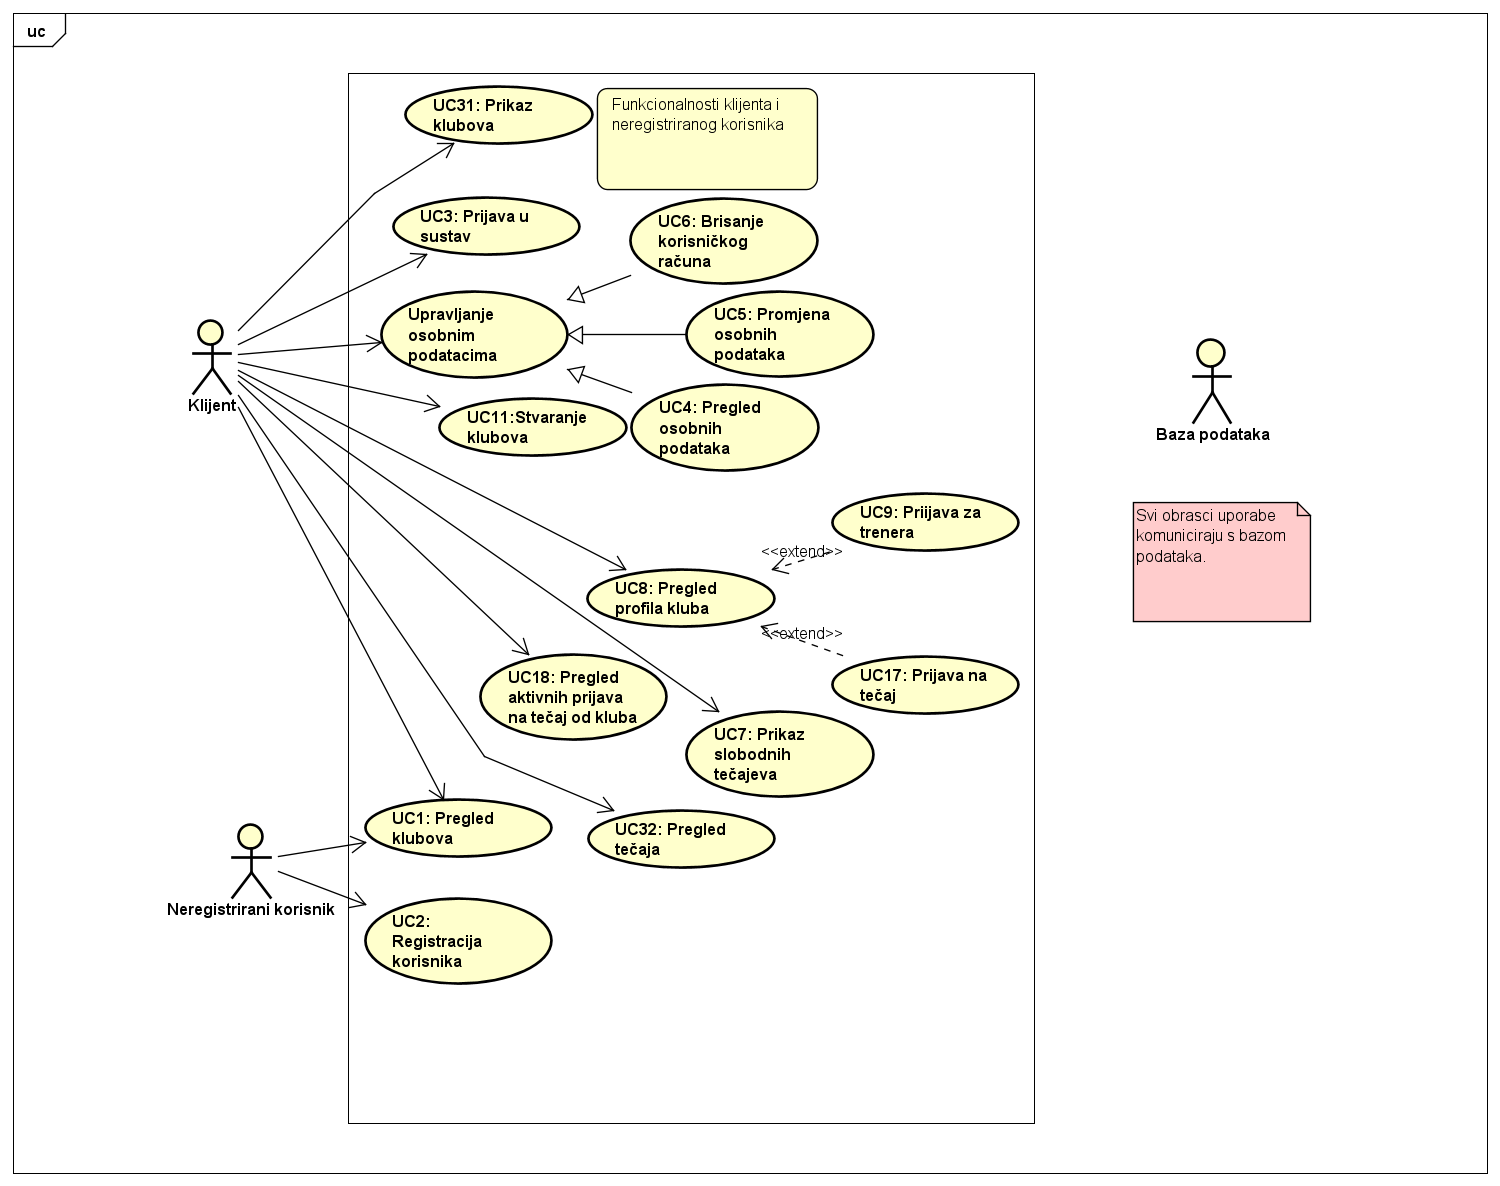
\includegraphics[width=\textwidth]{slike/Diagram1.png}
						\caption{Dijagram obrasca uporabe, funkcionalnost neregistriranog korisnika, klijenta i kluba}
						\label{fig:my_label}
					\end{figure}
					\begin{figure}[H]
						\centering
						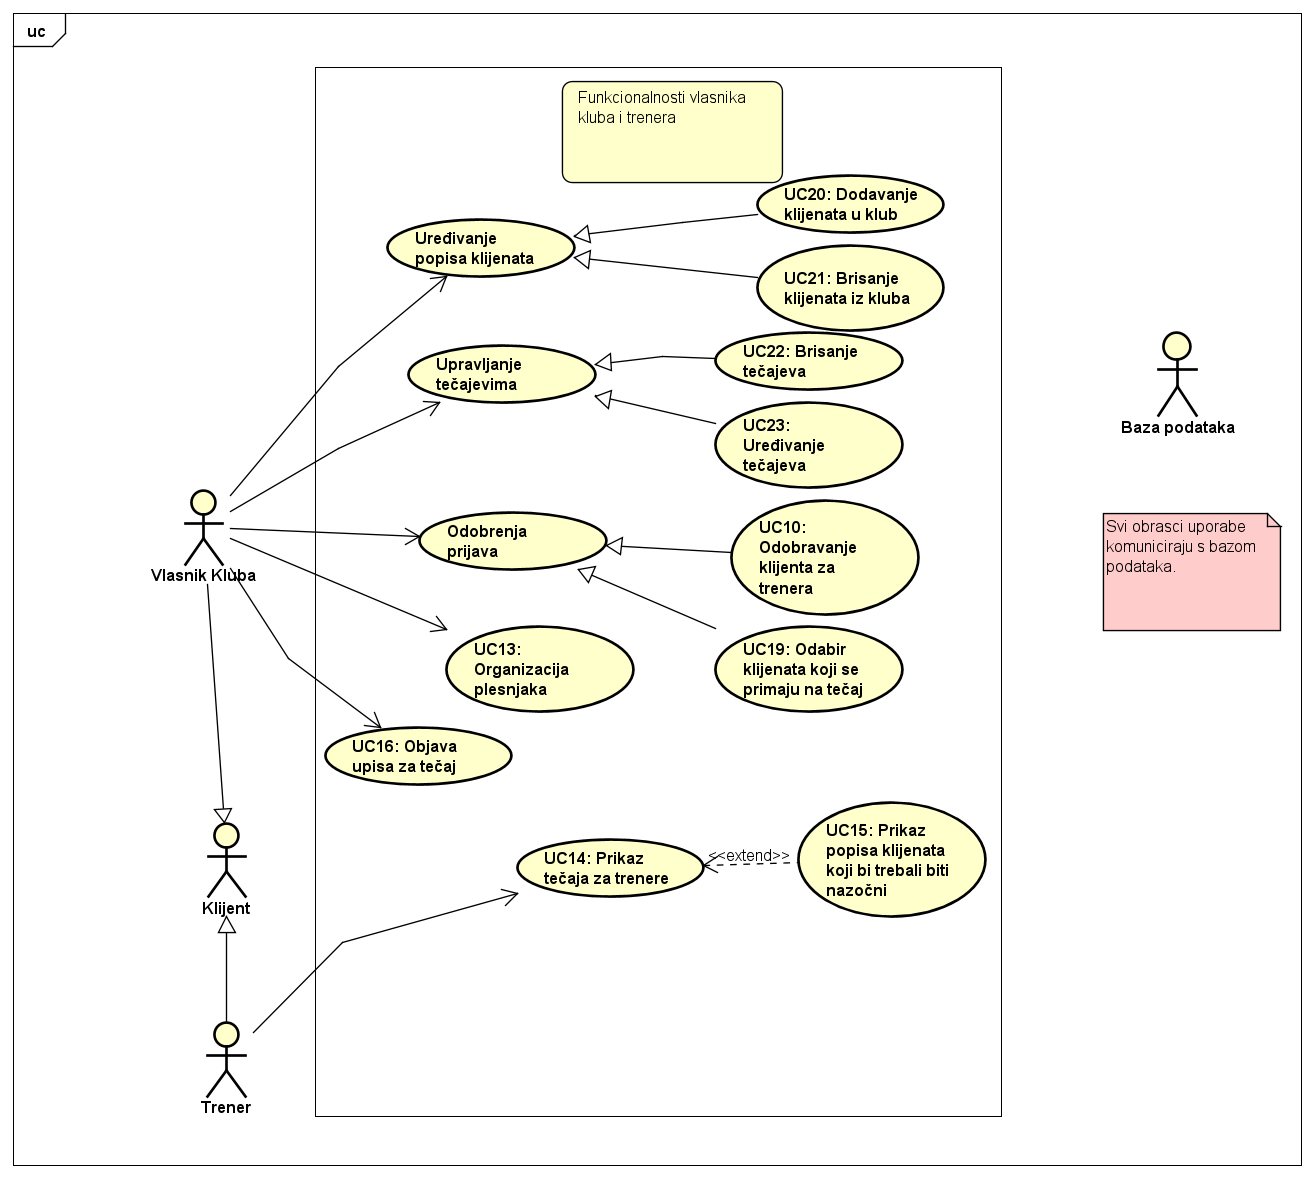
\includegraphics[width=\textwidth]{slike/Diagram2.png}
						\caption{Dijagram obrasca uporabe, funkcionalnost trenera i kluba}
						\label{fig:my_label}
					\end{figure}
					\begin{figure}[H]
						\centering
						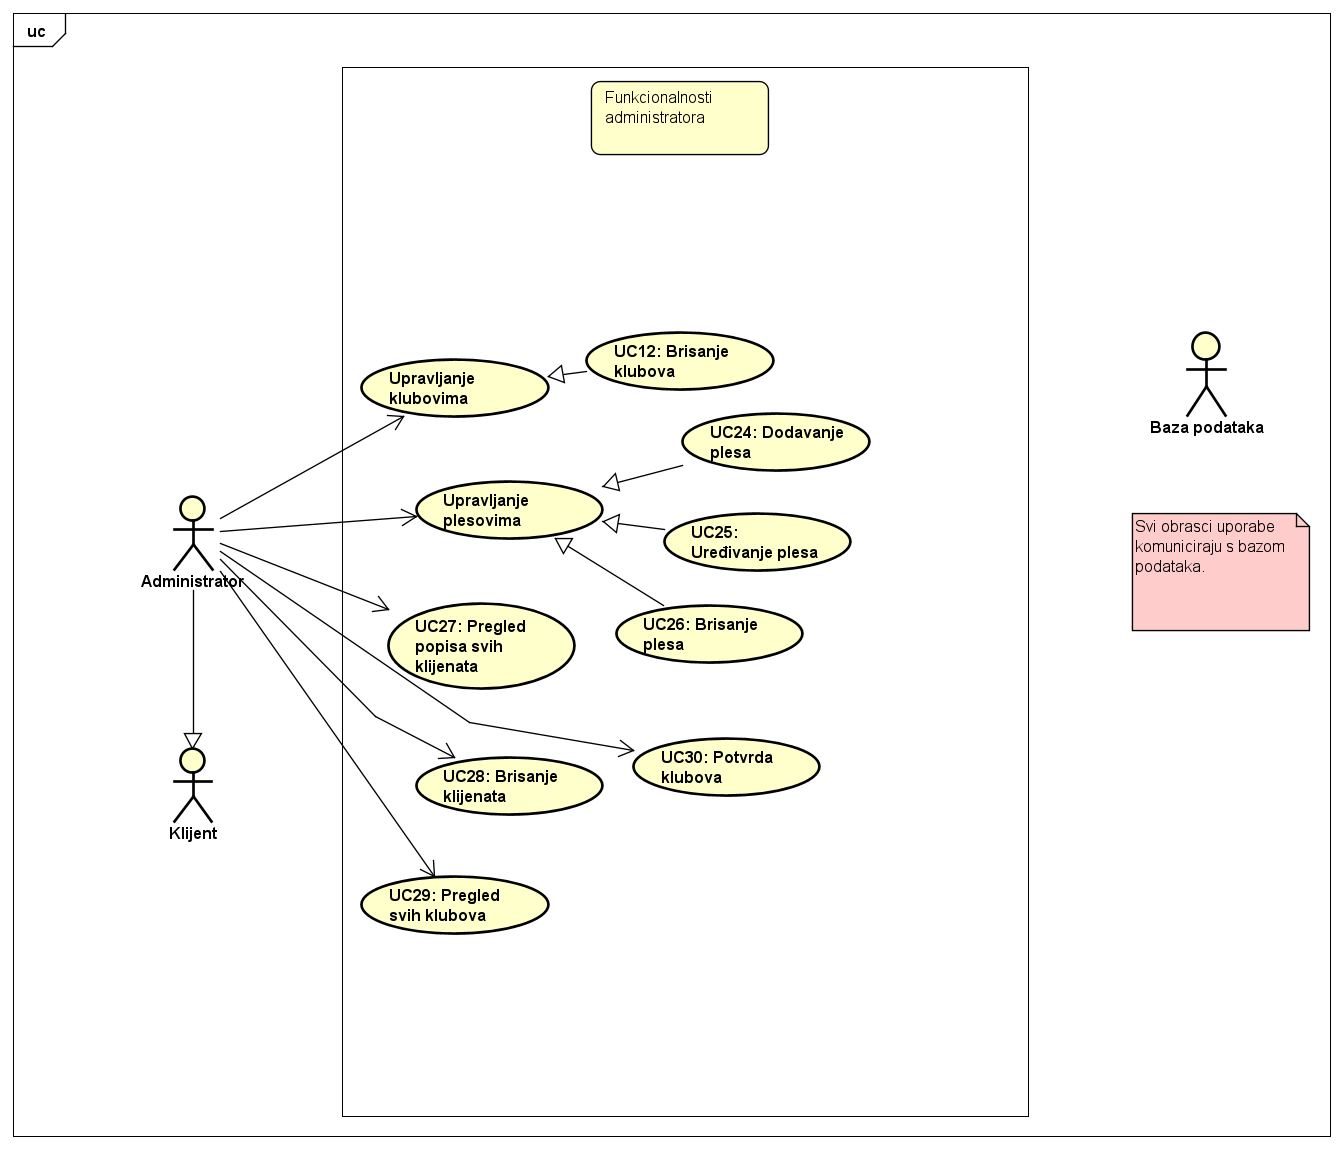
\includegraphics[width=\textwidth]{slike/Diagram3.png}
						\caption{Dijagram obrasca uporabe, funkcionalnost administratora}
						\label{fig:my_label}
					\end{figure}
			
			\eject
			\subsection{Sekvencijski dijagrami}
				
				\textbf{Obrasci uporabe: U31-prikaz klubova, UC8-Pregled profila kluba, UC9- prijava za trenera}\\
				
				Klijent šalje zahtjev za prikaz karte kako bi mogao odabrati klub.
				Poslužitelj dohvaća trenutne klubove i prikazuje ih. Odabirom kluba, poslužitelj iz baze podataka dohvaća osnovne podatke o klubu i prikazuje ih korisniku. Klijent odabire opciju prijave trenera. Poslužitelj isporučuje formu koja od korisnika traži predaju motivacijskog pisma i potvrde. Klijent predaje potrebne dokumente te prima poruku o uspješnoj pohrani prijave.
				
				\begin{figure}[H]
					\centering
					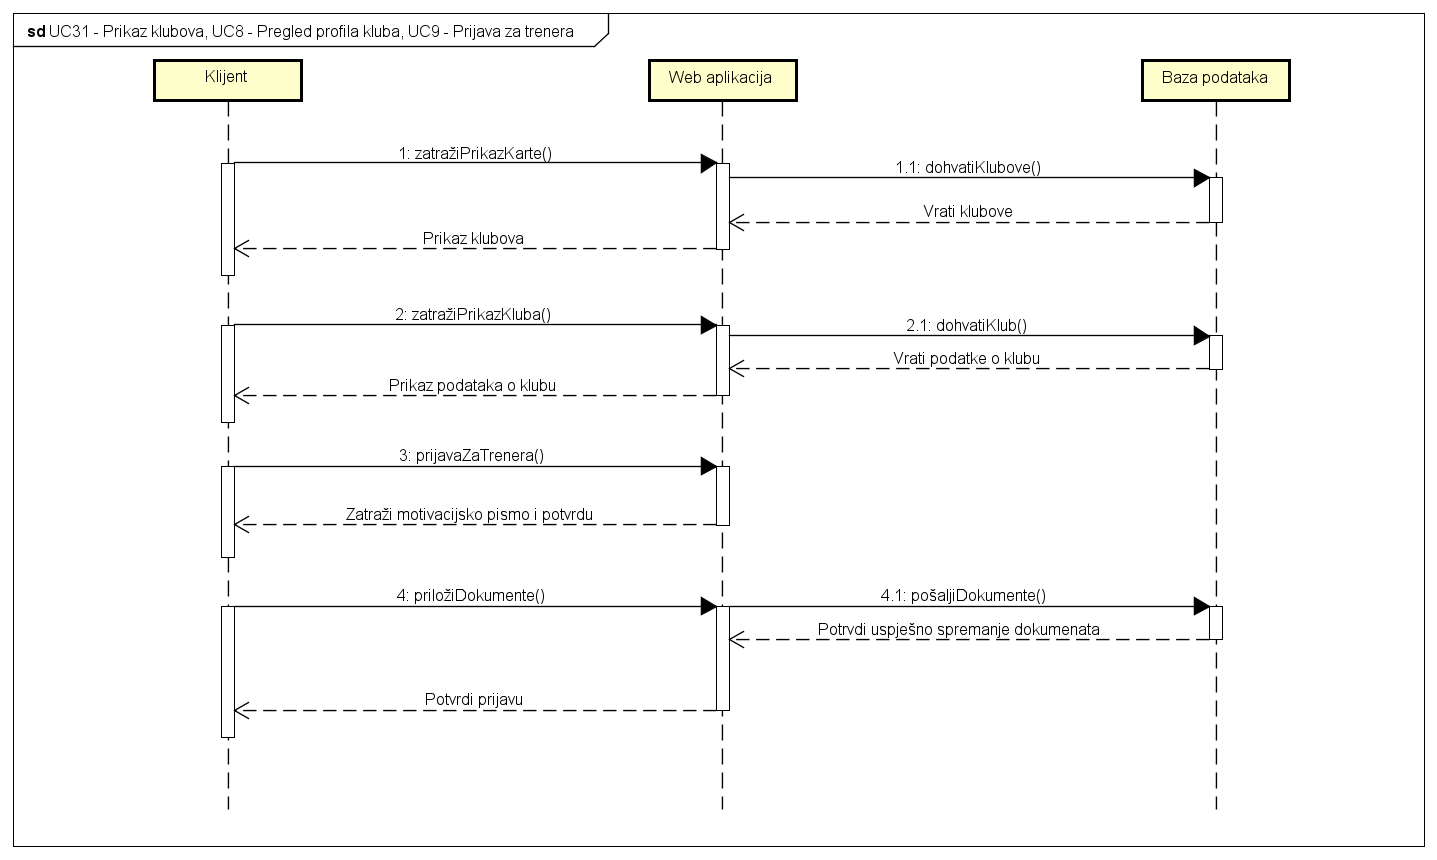
\includegraphics[width=\textwidth]{slike/seq_dijagram1.png}
					\caption{Sekvencijski dijagram za UC31, UC8 i UC9}
					\label{fig:my_label}
				\end{figure}
				\eject
				\textbf{Obrasci uporabe: UC7-prikaz tečajeva, UC32-Pregled tečaja, UC19- Odabir klijenta koji se primaju na tečaj}\\
			
				Vlasnik kluba šalje zahtjev za prikaz karte kako bi mogao odabrati tečaj. Poslužitelj dohvaća trenutne tečajeve i prikazuje ih. Odabirom tečaja, poslužitelj iz baze podataka dohvaća osnovne podatke o tečaju i prikazuje ih korisniku (vlasniku kluba). Vlasnik kluba odabire opciju pregleda prijava na tečaj. Poslužitelj dohvaća trenutne prijave na odabrani tečaj te ih prikazuje. Vlasnik kluba bira koje će klijente odabrat u grupu za tečaj. Pošlužitelj podatke o odabranim klijentima sprema u bazu. Pri završetku rada poslužitelj briše trenutne prijave iz baze.
			
				\begin{figure}[H]
					\centering
					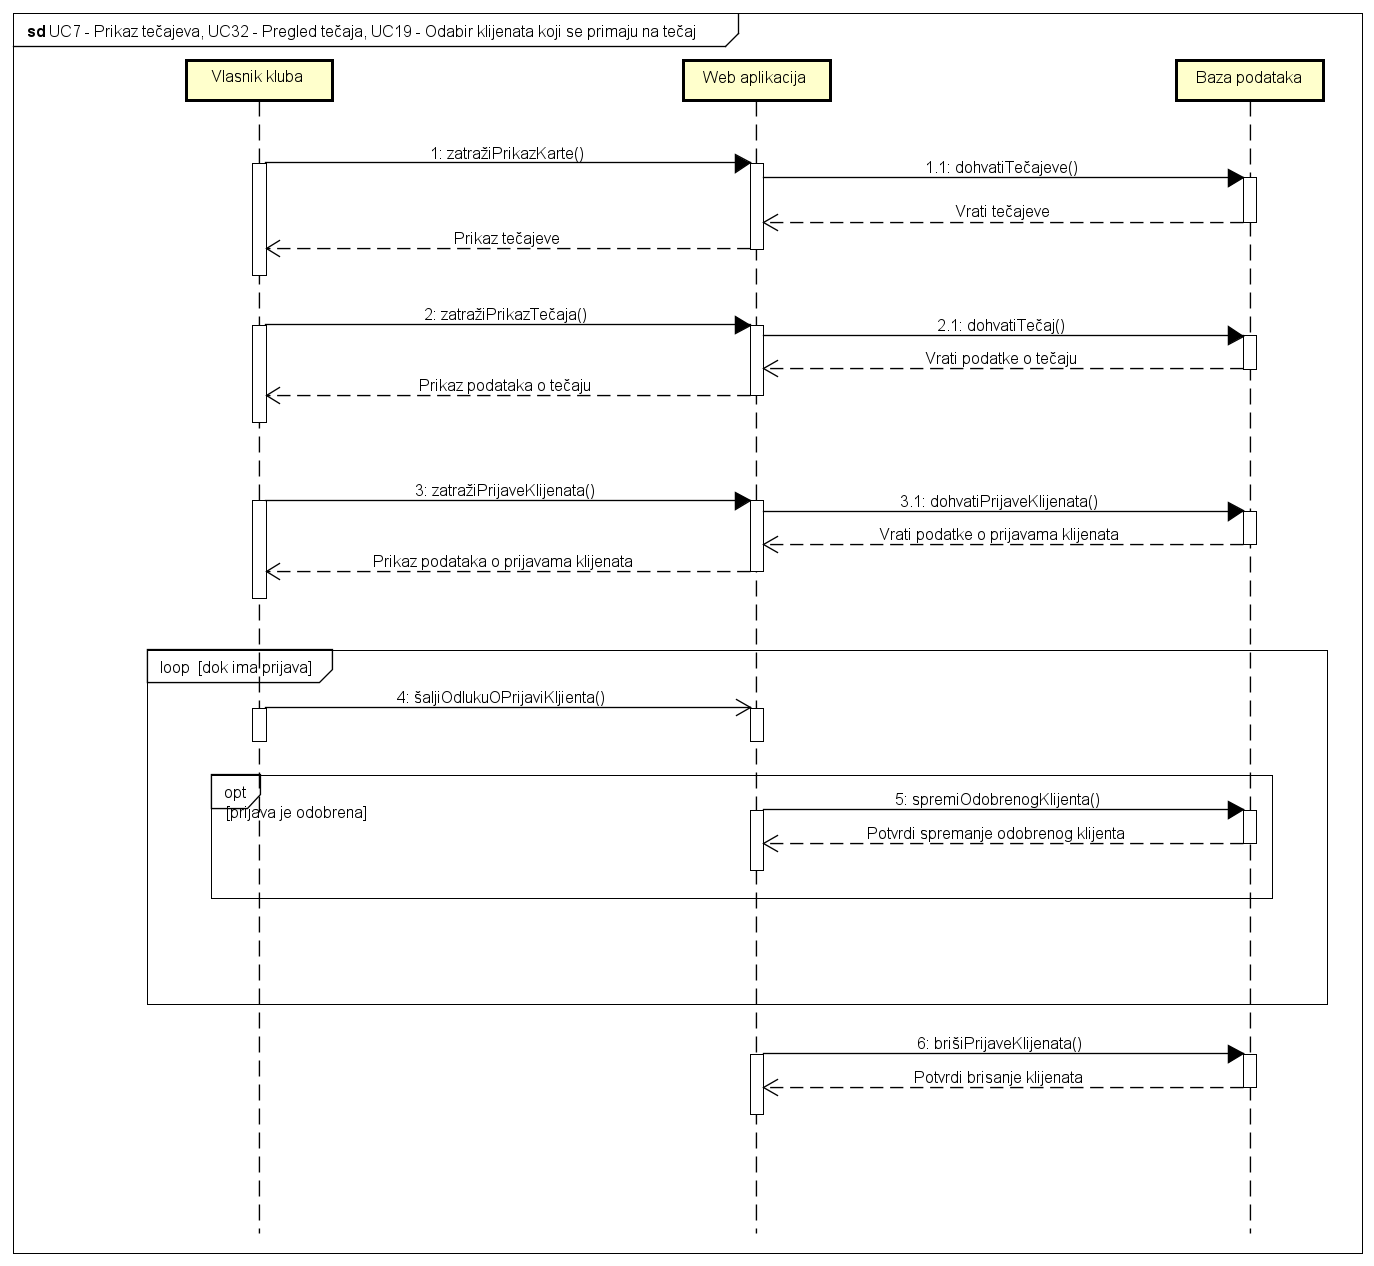
\includegraphics[width=\textwidth]{slike/seq_dijagram2.png}
					\caption{Sekvencijski dijagram za UC7, UC32 i UC19}
					\label{fig:my_label}
				\end{figure}
			\bigskip
			
				\textbf{Obrasci uporabe: UC13 - Organizacija plesnjaka}\\
				
				Vlasnik kluba šalje zahtjev za prikaz popisa svih dostupnih plesnjaka. Poslužitelj potom dohvaća sve dostupne plesnjake iz baze podataka i prikazuje ih korisniku (vlasniku kluba). Odabirom opcije dodavanja plesnjaka poslužitelj isporučuje formu koja od vlasnika kluba traži unos informacija za novi plesnjak. Vlasnik kluba ispunjava formu s potrebnim informacijama koje onda poslužitelj sprema u bazu podataka. Nakon spremanja poslužitelj zahtjeva od vlasnika kluba potvrdu o spremanju.
				
				\begin{figure}[H]
					\centering
					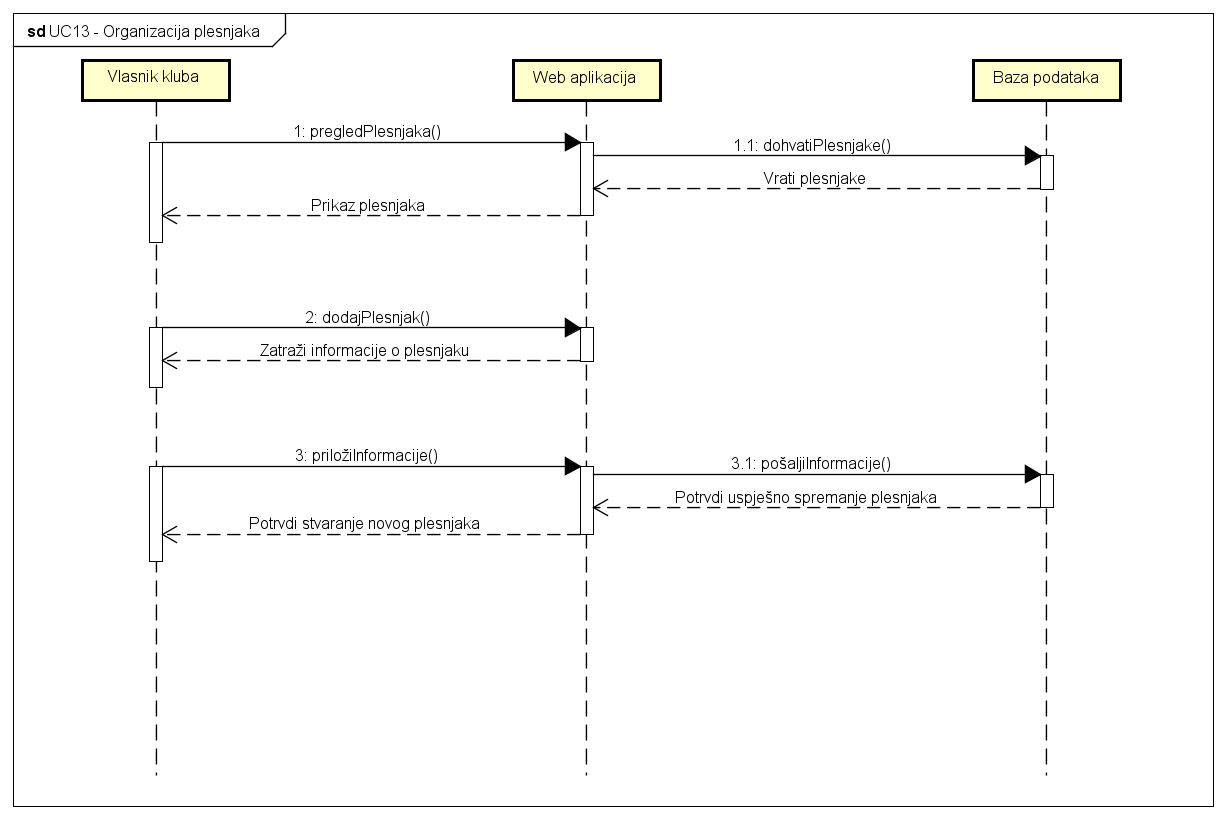
\includegraphics[width=\textwidth]{slike/seq_dijagram3.png}
					\caption{Sekvencijski dijagram za UC13}
					\label{fig:my_label}
				\end{figure}
			
		\newpage
			
				\textbf{Obrasci uporabe: UC11 - Stvaranje klubova, UC30 - Potvrda klubova}\\
				
				Klijent šalje zahtjev za stvaranjem novog kluba. Poslužitelj potom isporučuje formu koja od klijenta  traži informacije za novi klub. Popunjavanjem forme poslužitelj sprema informacije o novom klubu u bazu podataka te zatim traži od klijenta potvrdu o stvaranju istog. Administrator šalje zahtjev za potvrđivanje klubova. Poslužitelj iz baze podataka dohvaća popis svih nepotvrđenih klubova i prikazuje ih administratoru sustava. Sve dok postoje nepotvrđeni klubovi administrator šalje odluku hoće li određeni klub odobriti ili ne. Ako je klub odobren, poslužitelj tu informaciju sprema u bazu. Ako je administrator potvrdio klub klijent koji je poslao zahtjev postaje vlasnikom kluba. Na kraju poslužitelj briše zahtjeve iz baze.
				
				\begin{figure}[H]
					\centering
					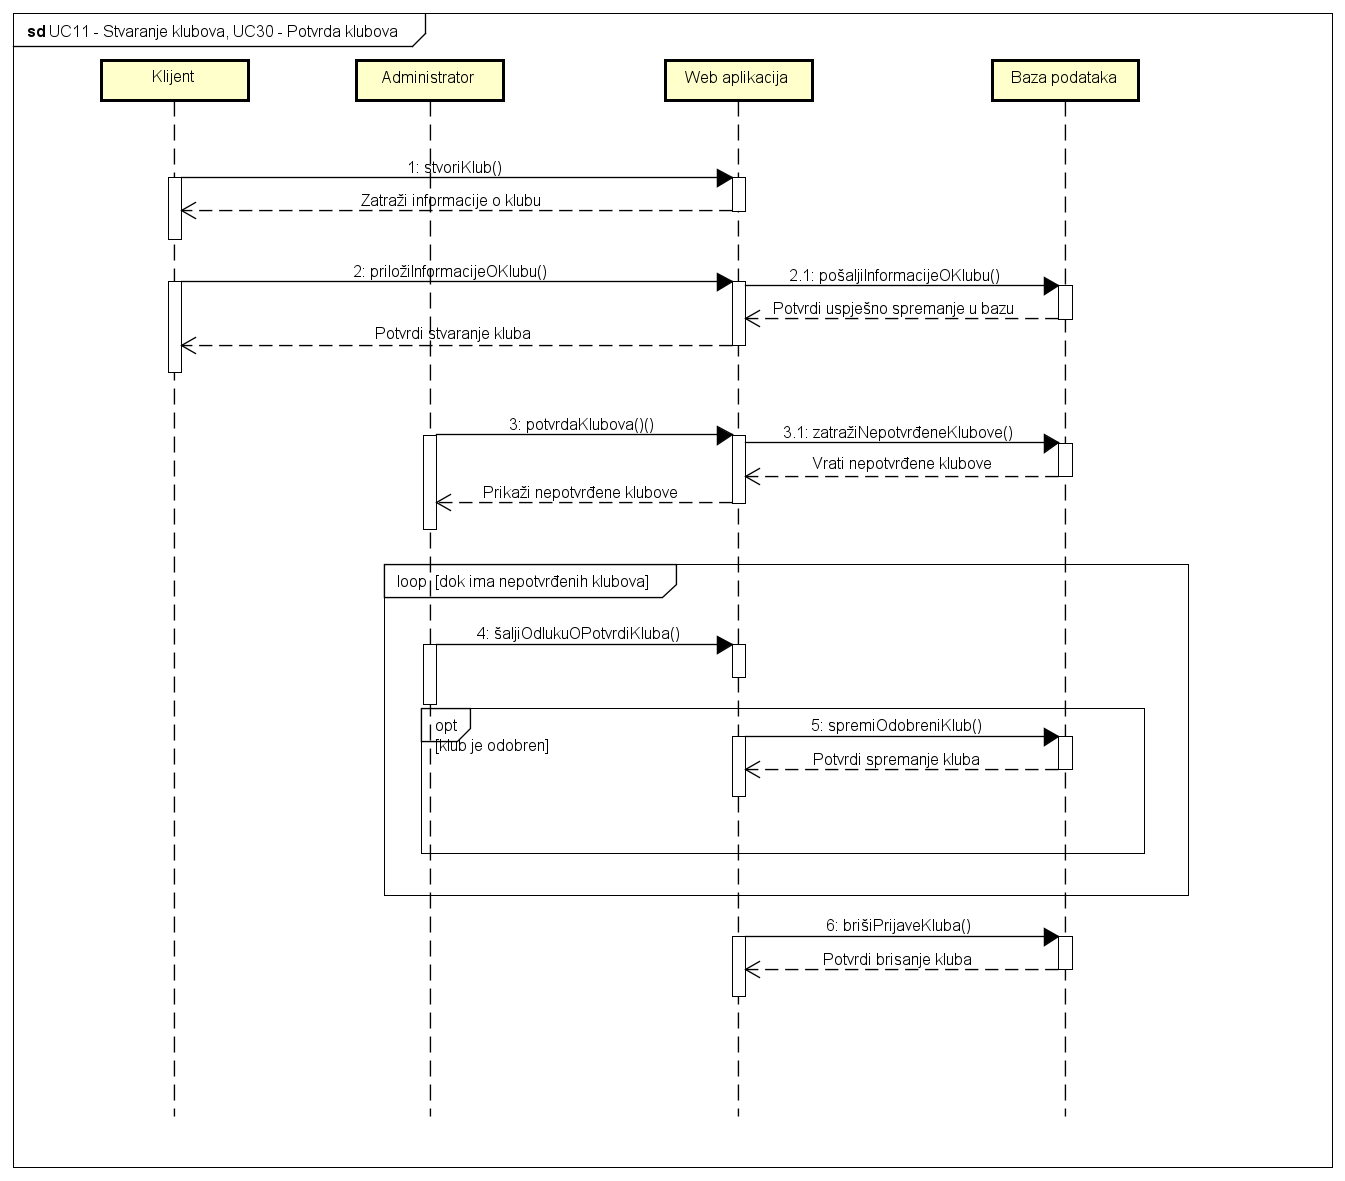
\includegraphics[width=\textwidth]{slike/seq_dijagram4.png}
					\caption{Sekvencijski dijagram za UC11, UC30}
					\label{fig:my_label}
				\end{figure}
	
		\section{Ostali zahtjevi}
		
		
			 \begin{packed_item}
			 	\item {Sustav mora omogućiti rad više korisnika u stvarnom vremenu}
			 	\item {Sustav treba kriptirati password koji korisnik unosi}
			 	\item {Veza s bazom podataka mora biti kvalitetno zaštićena te brza i otporna na vanjske greške}
			 	\item {Izvršavanje dijela programa koji pristupa bazi podataka ne smije trajati duže od par sekundi}
			 	\item {Korisničko sučelje i sustav moraju podržavati hrvatsku abecedu pri unosu i prikazu tekstualnog sadržaja}
			 	\item {Sustav treba biti implementiran kao web aplikacija koristeći objektno-orijentirane jezike}
			 	\item {Sustav mora biti lagan i intuitivan za korištenje, kako bi ga koristili korisnici bez dodatnih opširnih uputa}
			 	\item {Nadogradnja sustava ne smije narušavati postojeće funkcije sustava}
			 	\item {Neispravno korištenje korisničkog sučelja ne smije narušiti funkcionalnosti i rad sustava}
			 \end{packed_item}
			 
	
	\chapter{Arhitektura i dizajn sustava}
		

\section{ Opis arhitekture }
\textit{  Arhitektura našeg sustava sastoji se od tri podsustava koji su međusobno povezani : Web preglednik, Web poslužitelj i Baza podataka. }

		\begin{packed_item}
			\item \textbf{Web preglednik : } \textit{ Korisnik se služi web-aplikacijom putem web preglednika i pritom se obrađuju korisnikovi zahtjevi. Putem web-preglednika korisnik (klijent) šalje zahtjeve poslužitelju. Poslužitelj vraća odgovor korisniku u obliku html dokumenta putem HTTP protokola. Više o modelu komunikacije klijenta i poslužitelja slijedi u nastavku.}
			\item \textbf{Web poslužitelj : } \textit{ Web poslužitelj kontrolira rad web-aplikacije. On prima i obrađuje dolazne zahtjeve, šalje odgovore korisniku te po potrebi pristupa bazi podataka. }
			\item \textbf{Baza podataka : } \textit{Baza podataka nam služi za pohranu i manipulaciju podacima koji se koriste prilikom upotrebe aplikacije.}
			\bigskip
		\end{packed_item}
	     
	     	\begin{figure}[H]
	     	\centering
	     	
\includegraphics[width=\textwidth]{slike/arh.png}
	     	\caption{Arhitektura sustava}
	     	\label{fig:my_label}
	         \end{figure}
		 
	    \newpage
		\subsection{Stil arhitekture}
		\textit{Arhitektura sustava je oblikovana objektno usmjereno. Objektno usmjerena paradigma rezultira idealiziranim opisom sustava u obliku jednostavnog modela koji je prikazan UML dijagramima razreda koji slijede u nastavku. Objektno usmjereno oblikovanje podrazumijeva objekte neophodne za implementaciju te se takvo oblikovanje veže uz određene tehnologije.}
	
		
		\subsection{Organizacija sustava}

					\subsubsection{Model klijent-poslužitelj}
					\textit{ Organizaciju sustava s visoke razine apstrakcije možemo prikazati modelom klijent-poslužitelj. Klijent zahtjeva uslugu od strane poslužitelja, šalje mu zahtjev i po potrebi očekuje odgovor. Poslužitelj nudi određenu uslugu, prima i obrađuje dolazne zahtjeve te po potrebi šalje odgovor klijentu. Poslužitelj je također zadužen za komunikaciju s bazom podataka. Prednost ovakvog modela jest veća sigurnost i zaštita podataka jer se klijent povezuje s bazom podataka preko aplikacije. 
					Klijent i poslužitelj spojeni su na IP mrežu te komuniciraju preko HTTP protokola na aplikacijskom sloju i TCP protokola na transportnom sloju.}
		
				    
				    	\begin{figure}[H]
				    	\centering
				    	
\includegraphics[width=\textwidth]{slike/kp.png}
				    	\caption{Komunikacija klijent-poslužitelj}
				    	\label{fig:my_label}
				          \end{figure}
	
					
					\subsubsection{Baza podataka}
					\textit{ Odlučili smo se za relacijsku bazu podataka, implementiranu pomoću PostgreSQL-a. Relacijska baza podataka prikuplja podatke te ih organizira prema relacijskom modelu.To je podatkovna baza za koju vrijedi da su u njoj podaci vezani relacijama (tablicama) i prikladno su  strukturirani. To nam osigurava : laku manipulaciju podacima, sigurnost i nadzor nad podacima, podaci su postojani i trajno spremljeni.}
		
		
		\subsection{Organizacija aplikacije}
		\textit{ Za organizaciju aplikacije koristimo MVC arhitekturni obrazac koji razdvaja prezentaciju podataka (View), dohvat i manipulaciju podataka (Model) i upravljanje zahtjevima (Controller). Detaljnija organizacija aplikacije prikazana je slikom 4.3. }
		\bigskip
		

			\begin{figure}[H]
			\centering
			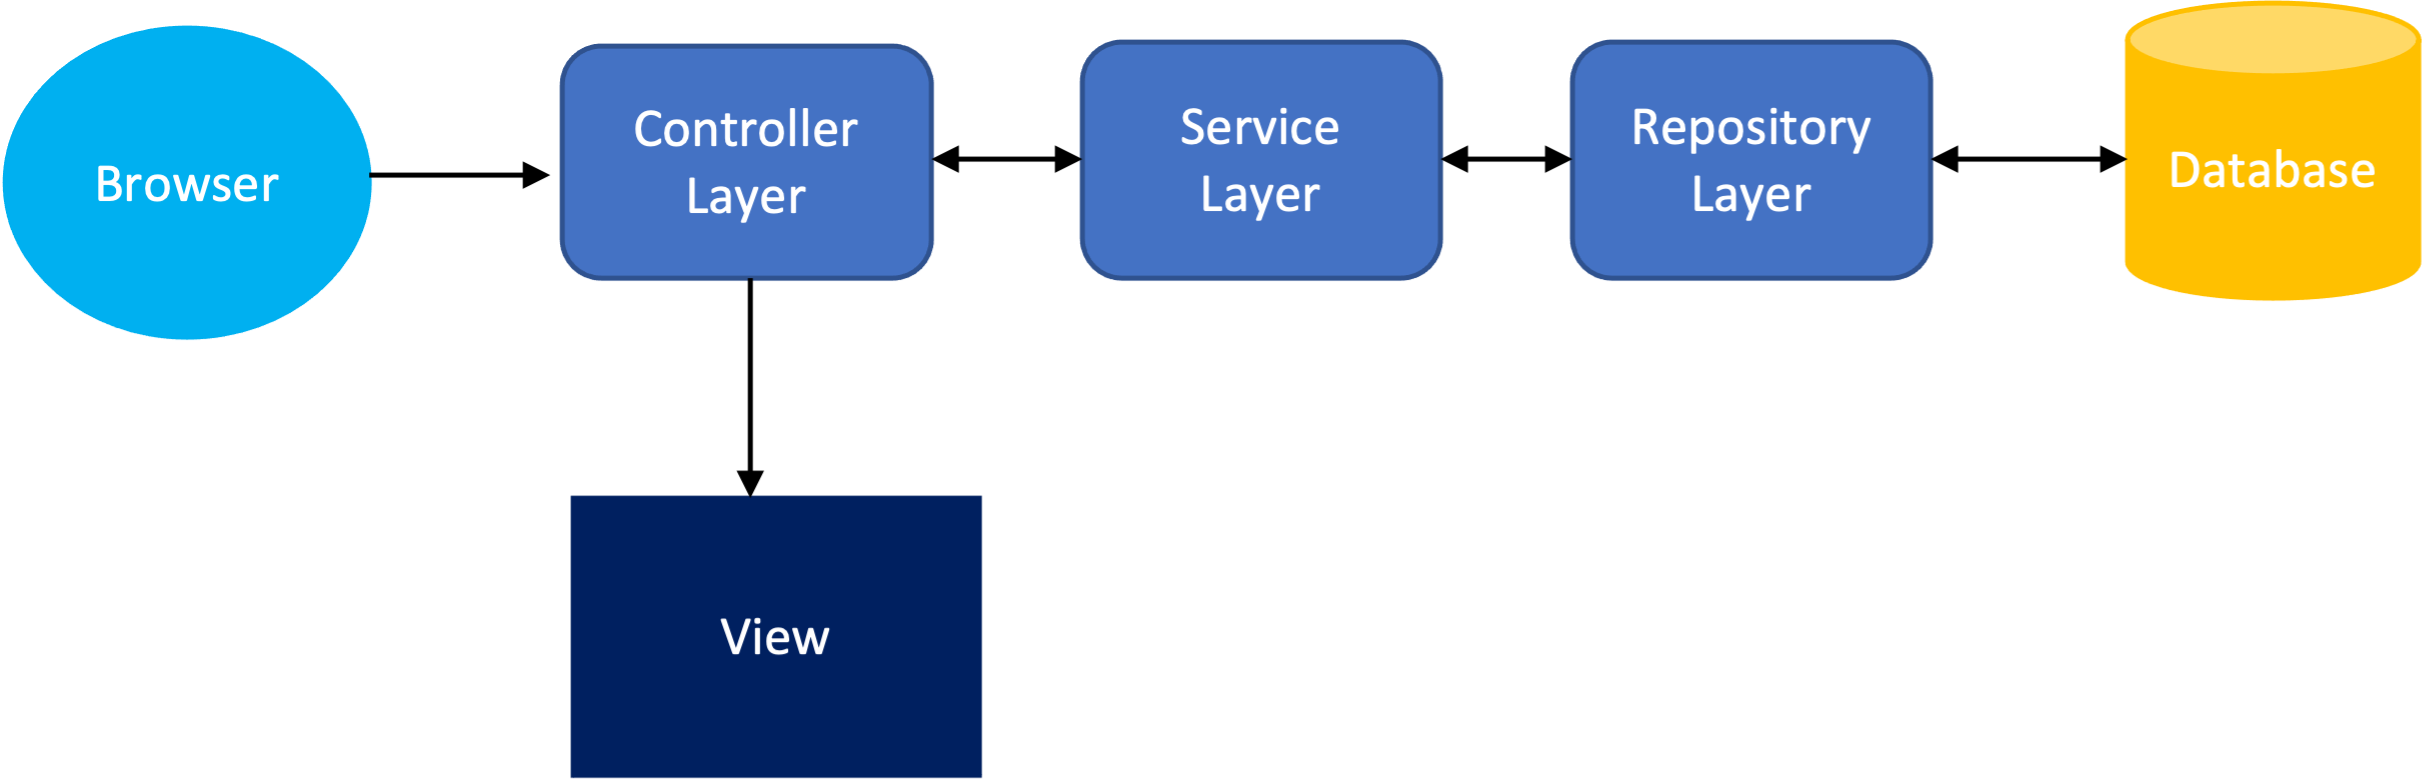
\includegraphics[width=\textwidth]{slike/mvc.png}
			\caption{MVC princip rada aplikacije}
			\label{fig:my_label}
		     \end{figure}
		
					\subsubsection{"front-end"}
					\textit{	U modelu klijent-poslužitelj, "klijentska strana aplikacije" odnosno dio web stranice s kojim korisnik(klijent) izravno komunicira naziva se front-end. Uključuje grafičko korisničko sučelje (GUI) odnosno sve što korisnici izravno doživljavaju: boje i stilove teksta, slike, grafikone i tablice, gumbe itd. Za izgradnju korisničkog sučelja odnosno front-enda koristimo alat React. }
					\bigskip 
					
					\subsubsection{"back-end"}
					\textit{	Poslužiteljska strana aplikacije pohranjuje i raspoređuje podatke te osigurava da sve na strani klijenta na web stranici radi dobro. To je dio web stranice koji korisnici ne mogu vidjeti i s njime ne mogu komunicirati odnosno to je ono što zovemo back-end. Za implementaciju back-enda koristimo Spring Boot zasnovan na razvojnom okviru Spring. }
				
	\newpage
	

		
		
		
		\section{Baza podataka}
		
		\textit{U bazi su kreirane relacije koje omogućavaju jednostavnu manipulaciju podacima (dodavanje, brisanje, izmjenjivanje i dohvat podataka). Sve relacije i entiteti uređeni su na 3. normalnu formu kako ne bi došlo do redundantnosti podataka. Da bi se lakše prikazala struktura korištene baze podataka, kreiran je relacijski dijagram baze podataka koji slijedi u nastavku. }
		
			\subsection{Dijagram baze podataka}	
		\begin{figure}[H]
			\centering
			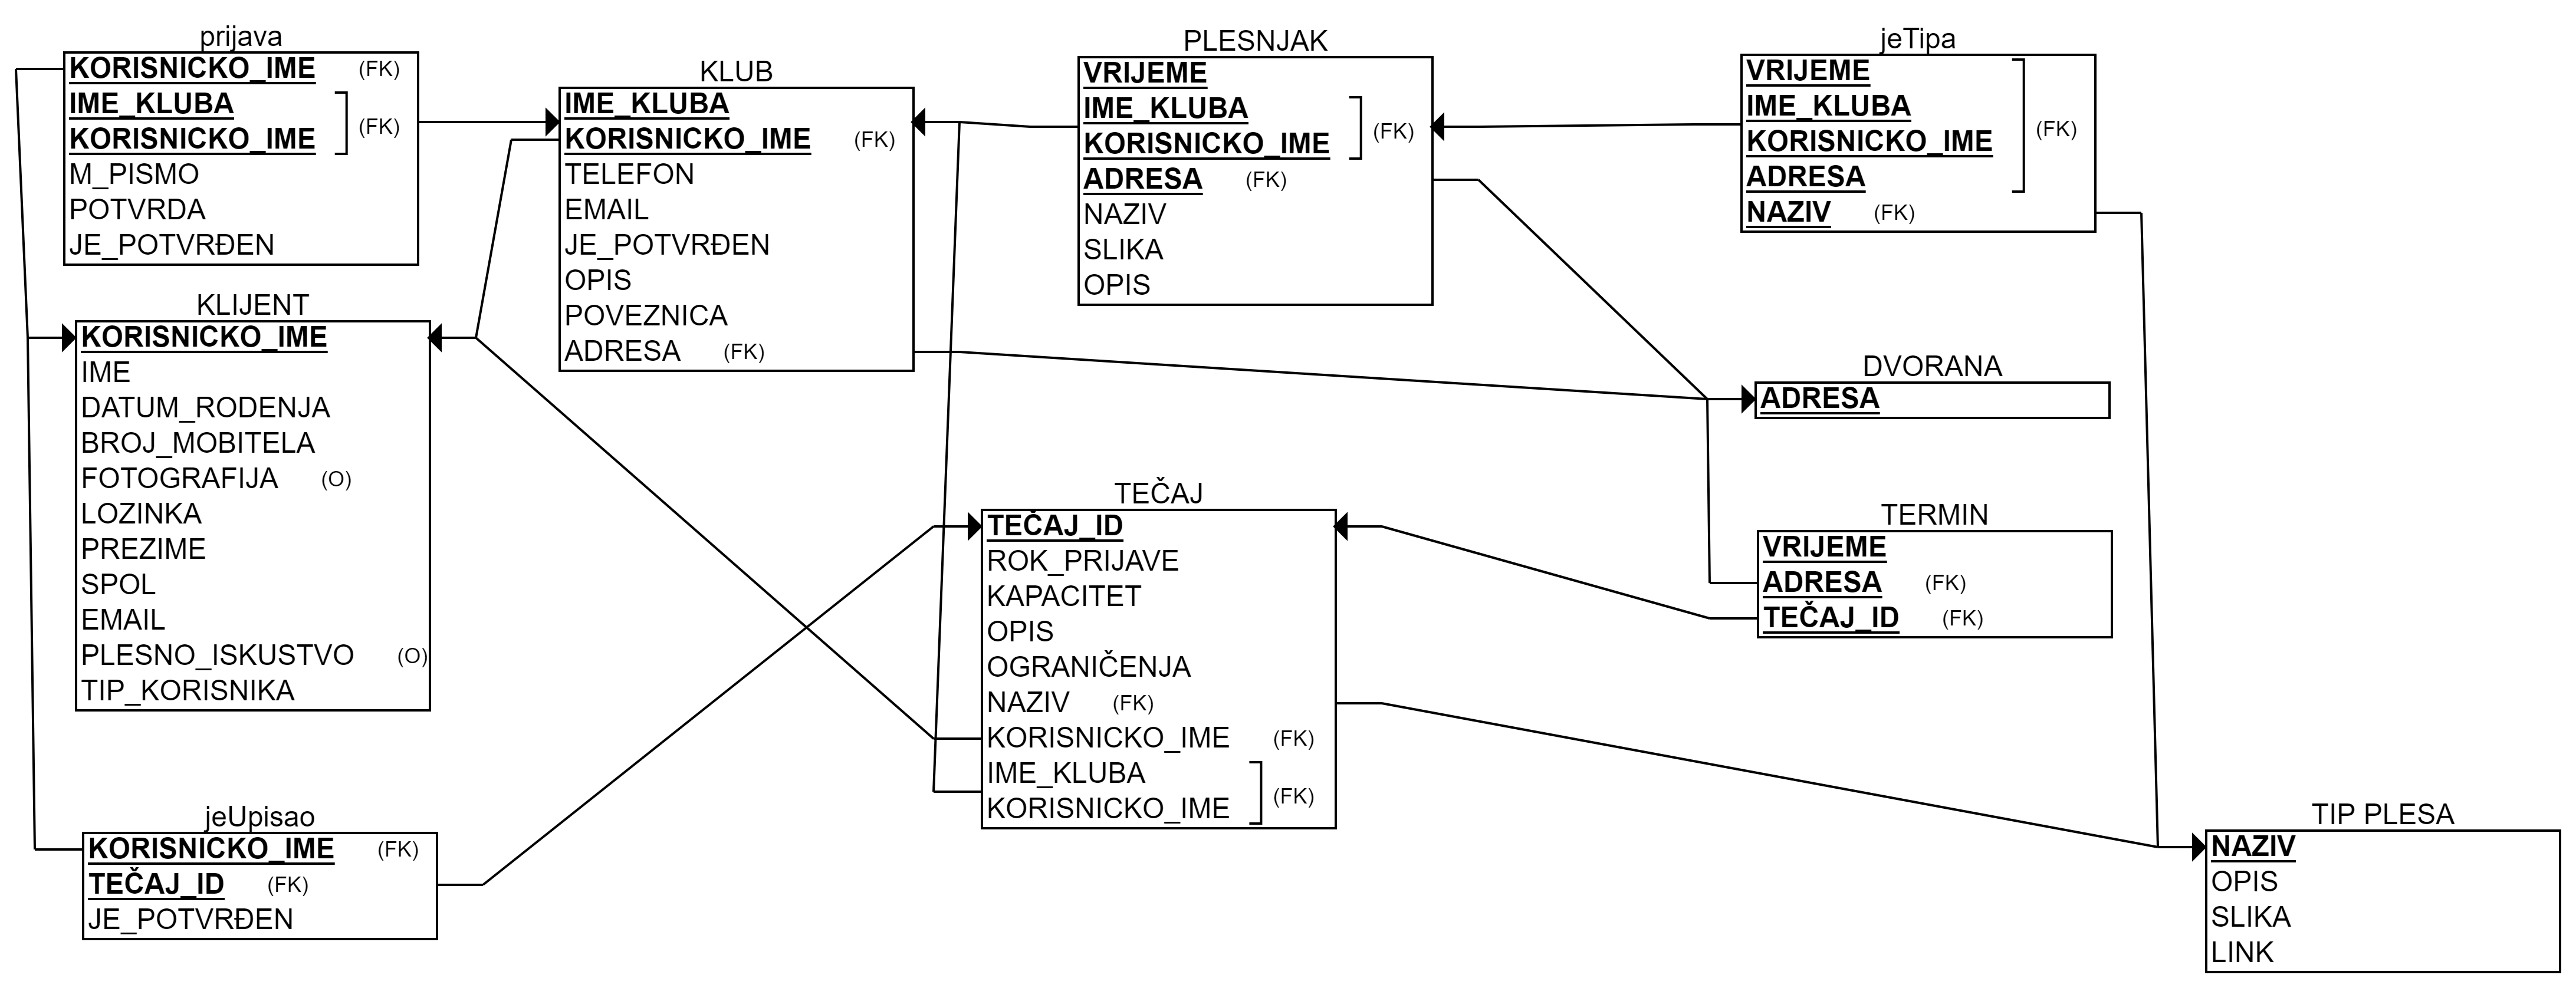
\includegraphics[width=\textwidth]{slike/baza.png}
			\caption{Relacijski dijagram baze podataka}
			\label{fig:my_label}
		\end{figure}
	
		
		\subsubsection{ Detaljnije o bazi }
		 Baza se sastoji od tablica (relacija) koje su definirane svojim imenom i skupom atributa. Baza podataka ove aplikacije sastoji se od sljedećih entiteta:
		 	\begin{packed_item}
		 		\item{Prijava}
		 		\item{Klijent}
		 		\item{JeUpisao}
		 		\item{Klub}
		 		\item{Plesnjak}
		 		\item{Tečaj}
		 		\item{jeTipa}
		 		\item{Dvorana}
		 		\item{Termin}
		 		\item{TipPlesa}
		 		
		 		\end{packed_item}
		 
		
		
			\subsection{Opis tablica}
			

				\textit{ Prva ćelija svake tablice označava njeno ime. U prvom stupcu navedeni su atributi tog entiteta, u drugom stupcu naveden je tip varijable, a u trećem opis svakog pojedinog atributa. Svjetlozelenom bojom označeni su primarni ključevi. Svjetlo plavom označeni su strani ključevi. Ukoliko je strani ključ također dio ključa, to je navedeno u opisu.}
				
				\subsubsection{Klijent}
				\textit{ Ovaj entitet  sadržava sve informacije o korisniku aplikacije kao što su korisničko ime, lozinka, ime, prezime, datum rođenja, broj mobitela, fotografija, spol, email, plesno iskustvo te koji je tip korisnika.}
				
				
				\begin{longtblr}[
					label=none,
					entry=none
					]{
						width = \textwidth,
						colspec={|X[12,l]|X[8, l]|X[20, l]|}, 
						rowhead = 1,
					} %definicija širine tablice, širine stupaca, poravnanje i broja redaka naslova tablice
					\hline \multicolumn{3}{|c|}{\textbf{KLIJENT}} & {\textbf{TIP}}	& {\textbf{OPIS}} \\ \hline[3pt]
					\SetCell{LightGreen}KORISNICKO\textunderscore IME & VARCHAR	&  Korisničko ime s kojim se korisnik prijavljuje	\\ \hline
					LOZINKA & VARCHAR	&  	Lozinka s kojom se korisnik prijavljuje	\\ \hline 
					IME	& VARCHAR &   Korisnikovo ime	\\ \hline 
					PREZIME & VARCHAR	&  Korisnikovo prezime		\\ \hline 
					DATUM\textunderscore RODENJA & DATE &  Korisnikov datum rođenja \\ \hline 
					BROJ\textunderscore MOBITELA & VARCHAR	&  	Korisnikov broj mobitela	\\ \hline 
					FOTOGRAFIJA & VARCHAR	&  	Put do korisnikove fotografije na serveru, OPCIONALNO	\\ \hline
					SPOL & VARCHAR(1)	&  	Korisnikov spol	\\ \hline
					EMAIL & VARCHAR	&  	Korisnikov email	\\ \hline  
					PLESNO\textunderscore ISKUSTVO & VARCHAR	&  	Opis korisikovog plesnog iskustva, OPCIONALNO	\\ \hline 
					TIP\textunderscore KORISNIKA & VARCHAR	&  	Jedan od: ADMINISTRATOR / VLASNIK KLUBA	\\ \hline 
				\end{longtblr}
			\newpage
			
			
			 \subsubsection{Dvorana}
			 \textit{Ovaj entitet sadržava informacije o plesnoj dvorani odnosno njenu adresu}
				
				\begin{longtblr}[
					label=none,
					entry=none
					]{
						width = \textwidth,
						colspec={|X[12,l]|X[8, l]|X[20, l]|}, 
						rowhead = 1,
					} %definicija širine tablice, širine stupaca, poravnanje i broja redaka naslova tablice
					\hline \multicolumn{3}{|c|}{\textbf{DVORANA}} & {\textbf{TIP}}	& {\textbf{OPIS}} \\ \hline[3pt]
					\SetCell{LightGreen}ADRESA & VARCHAR	&  Adresa plesne dvorane	\\ \hline
					
				\end{longtblr}
			\bigskip
			\bigskip
			
			  \subsubsection{Klub}
			 \textit{Ovaj entitet sadržava sve informacije koje su bitne za klub kao što su njegovo ime, korisnicko ime klijenta koji je vlasnik kluba, email od kluba, broj telefona od kluba, potvrdu o stanju (je li administrator potvrdio klub), opis kluba, poveznica na stranicu s grupama za upis te adresu kluba. }
			 	
	
				
				\begin{longtblr}[
					label=none,
					entry=none
					]{
						width = \textwidth,
						colspec={|X[12,l]|X[8, l]|X[20, l]|}, 
						rowhead = 1,
					} %definicija širine tablice, širine stupaca, poravnanje i broja redaka naslova tablice
					\hline \multicolumn{3}{|c|}{\textbf{KLUB}} & {\textbf{TIP}}	& {\textbf{OPIS}} \\ \hline[3pt]
					\SetCell{LightGreen}IME\textunderscore KLUBA & VARCHAR	&  Naziv kluba	\\ \hline
					\SetCell{LightBlue}KORISNICKO\textunderscore IME & VARCHAR	&  Dio ključa, korisničko ime klijenta koji je vlasnik kluba	\\ \hline
					EMAIL & VARCHAR	&  	Email od kluba	\\ \hline  
					TELEFON & VARCHAR	&  	Broj telefona od kluba	\\ \hline 
					JE\textunderscore POTVRĐEN & BOOLEAN	&  	Stanje je li administrator potvrdio klub	\\ \hline 
					OPIS	& VARCHAR &   Kratki opis kluba	\\ \hline 
					POVEZNICA & VARCHAR	&  	Poveznica na stranicu s grupama za upis	\\ \hline 
					\SetCell{LightBlue}ADRESA & VARCHAR	&  Adresa sjedišta kluba	\\ \hline
	
				\end{longtblr}
			\newpage
			
			 \subsubsection{Prijava}
			\textit{Ovaj entitet sadržava sve važne informacije korisnika koji ispunjava prijavu da postane  trener u klubu. Te informacije su navedene kao atributi : korisnicko ime trenera, ime kluba, korisnicko ime vlasnika kluba, motivacijsko pismo, potvrda korisnikove sposobnosti te stanje potvrde (je li vlasnik kluba potvrdio korisnika kao trenera). }
				
				\begin{longtblr}[
					label=none,
					entry=none
					]{
						width = \textwidth,
						colspec={|X[12,l]|X[8, l]|X[20, l]|}, 
						rowhead = 1,
					} %definicija širine tablice, širine stupaca, poravnanje i broja redaka naslova tablice
					\hline \multicolumn{3}{|c|}{\textbf{PRIJAVA}} & {\textbf{TIP}}	& {\textbf{OPIS}} \\ \hline[3pt]
					\SetCell{LightBlue}KORISNICKO\textunderscore IME TRENERA & VARCHAR	&  Dio ključa, korisničko ime klijenta koji želi postati trener	\\ \hline
					\SetCell{LightBlue}IME\textunderscore KLUBA & VARCHAR	&  Dio ključa, naziv kluba u kojem korisnik želi biti trener	\\ \hline
					\SetCell{LightBlue}KORISNICKO\textunderscore IME VLASNIKA & VARCHAR	&  Dio ključa, korisničko ime vlasnika kluba u kojem korisnik želi biti trener	\\ \hline
					
					M\textunderscore PISMO & VARCHAR	&  	Motivacijsko pismo trenera	\\ \hline  
					POTVRDA & VARCHAR	&  	Put do korisnikove potvrde sposobnosti, na serveru	\\ \hline  	
					JE\textunderscore POTVRDEN & BOOLEAN	&  	Stanje je li vlasnik kluba potvrdio trenera	\\ \hline  		
				\end{longtblr}
			\bigskip
			
			\subsubsection{Tip plesa}
			\textit{Ovaj entitet sadrži sve važne informacije o plesu, a to su : naziv, opis,slika, link }
			
				
					\begin{longtblr}[
					label=none,
					entry=none
					]{
						width = \textwidth,
						colspec={|X[12,l]|X[8, l]|X[20, l]|}, 
						rowhead = 1,
					} %definicija širine tablice, širine stupaca, poravnanje i broja redaka naslova tablice
					\hline \multicolumn{3}{|c|}{\textbf{TIP\textunderscore PLESA}} & {\textbf{TIP}}	& {\textbf{OPIS}} \\ \hline[3pt]
					\SetCell{LightGreen}NAZIV & VARCHAR	&  Ime plesa	\\ \hline
					
					OPIS & VARCHAR	&  	Kratki opis plesa	\\ \hline 
					SLIKA	& VARCHAR &   Put do slike plesa, na serveru	\\ \hline 
					LINK & VARCHAR	&  Link na videozapis plesa		\\ \hline 
					
				\end{longtblr}
			
			\newpage
			
				\subsubsection{Plesnjak}
			\textit{ Ovaj entitet sadrži sve važne informacije o održavanju plesnjaka kao što su vrijeme održavanja, ime kluba koji ga održava, korisničko ime vlasnika kluba koji organizira plesnjak, adresa održavanja plesnjaka, naziv plensjaka, slika i opis.}
			
			\begin{longtblr}[
				label=none,
				entry=none
				]{
					width = \textwidth,
					colspec={|X[12,l]|X[8, l]|X[20, l]|}, 
					rowhead = 1,
				} %definicija širine tablice, širine stupaca, poravnanje i broja redaka naslova tablice
				\hline \multicolumn{3}{|c|}{\textbf{PLESNJAK}} & {\textbf{TIP}}	& {\textbf{OPIS}} \\ \hline[3pt]
				\SetCell{LightGreen}VRIJEME & DATE	&  	Vrijeme održavanja plesnjaka\\ \hline
				\SetCell{LightBlue}IME\textunderscore KLUBA & VARCHAR	&  Dio ključa, naziv kluba koji organizira plesnjak	\\ \hline
				\SetCell{LightBlue}KORISNICKO\textunderscore IME & VARCHAR	&  Dio ključa, vlasnik kluba koji organizira plesnjak	\\ \hline
				\SetCell{LightBlue}ADRESA & VARCHAR	&  Dio ključa, mjesto održavanja plesnjaka	\\ \hline
				
				NAZIV & VARCHAR	&  	Naziv plesnjaka	\\ \hline  
				SLIKA & VARCHAR	&  	Put do slike o plesnjaku, na serveru	\\ \hline  
				OPIS	& VARCHAR &   Kratki opis plesnjaka	\\ \hline 
				
			\end{longtblr}
		
			\subsubsection{Termin}
		\textit{Ovaj entitet sadrži sve važne informacije o terminu održavanja određenog tečaja, a to je : vrijeme održavanja, adresa održavanja i ID tečaja koji se održava.}
		
		\begin{longtblr}[
			label=none,
			entry=none
			]{
				width = \textwidth,
				colspec={|X[12,l]|X[8, l]|X[20, l]|}, 
				rowhead = 1,
			} %definicija širine tablice, širine stupaca, poravnanje i broja redaka naslova tablice
			\hline \multicolumn{3}{|c|}{\textbf{TERMIN}} & {\textbf{TIP}}	& {\textbf{OPIS}} \\ \hline[3pt]
			\SetCell{LightGreen}VRIJEME & DATE	&  Vrijeme održavanja tečaja	\\ \hline
			\SetCell{LightBlue}ADRESA & VARCHAR	&  Dio ključa, adresa dvorane gdje se održava tečaj	\\ \hline
			\SetCell{LightBlue}TECAJ\textunderscore ID & INT	&  Dio ključa, ID tečaja koji se održava	\\ \hline
			
		\end{longtblr}
	
	\newpage
	
		
			\subsubsection{Plesnjak tipa}
		\textit{Ovaj entitet sadržava sve važne informacije o tipu plesnjaka koji postoji. Kako se na plesnjaku može plesati više vrsta plesova, ovdje su bitne informacije : vrijeme održavanja plesnjaka, ime kluba koji ga organizira, korisnicko ime vlasnika kluba, adresa održavanja i naziv plesa koji se pleše na plesnjaku.}
				
				\begin{longtblr}[
					label=none,
					entry=none
					]{
						width = \textwidth,
						colspec={|X[12,l]|X[8, l]|X[20, l]|}, 
						rowhead = 1,
					} %definicija širine tablice, širine stupaca, poravnanje i broja redaka naslova tablice
					\hline \multicolumn{3}{|c|}{\textbf{PLESNJAK\textunderscore TIPA}} & {\textbf{TIP}}	& {\textbf{OPIS}} \\ \hline[3pt]
					\SetCell{LightBlue}VRIJEME & DATE	&  Dio ključa, vrijeme održavanja plesnjaka	\\ \hline
					\SetCell{LightBlue}IME\textunderscore KLUBA & VARCHAR	&  Dio ključa, naziv kluba koji organizira plesnjak	\\ \hline
					\SetCell{LightBlue}KORISNICKO\textunderscore IME & VARCHAR	&  Dio ključa, vlasnik kluba koji organizira plesnjak	\\ \hline
					\SetCell{LightBlue}ADRESA & VARCHAR	&  Dio ključa, mjesto održavanja plesnjaka	\\ \hline
					\SetCell{LightBlue}NAZIV\textunderscore PLESA & VARCHAR	&  Dio ključa, naziv plesa koji se pleše na plesnjaku	\\ \hline
			
				\end{longtblr}
			\bigskip
			\bigskip
			
				\subsubsection{Upis tecaj}
			\textit{Ovaj entitet sadrži sve važne informacije o upisu klijenta na određeni tečaj, a to su : korisničko ime tog klijenta, ID tečaja koji se upisuje i stanje (je li upis potvrđen).}
			
			\begin{longtblr}[
				label=none,
				entry=none
				]{
					width = \textwidth,
					colspec={|X[12,l]|X[8, l]|X[20, l]|}, 
					rowhead = 1,
				} %definicija širine tablice, širine stupaca, poravnanje i broja redaka naslova tablice
				\hline \multicolumn{3}{|c|}{\textbf{UPIS\textunderscore TECAJ}} & {\textbf{TIP}}	& {\textbf{OPIS}} \\ \hline[3pt]
				\SetCell{LightBlue}KORISNICKO\textunderscore IME & VARCHAR	&  Dio ključa, korisničko ime klijenta	\\ \hline
				\SetCell{LightBlue}TECAJ\textunderscore ID & INT	&  Dio ključa, ID tečaja koji se upisuje	\\ \hline
				
				JE\textunderscore POTVRDEN & BOOLEAN	&  	Stanje je li korisnikov upis na tečaj potvrđen	\\ \hline 
			\end{longtblr}
			
			\newpage
			
			
				\subsubsection{Tecaj}
			\textit{Ovaj entitet sadržava sve važne informacije o pojedinom tečaju, a to su njegov ID, rok za prijavu na tečaj, kapacitet grupe na tečaju, kratki opis tečaja, ograničenja, naziv plesa za koji se tečaj održava, korisnicko ime trenera, ime kluba koji održava tečaj  te korisničko ime vlasnika tog kluba.}
				
				\begin{longtblr}[
					label=none,
					entry=none
					]{
						width = \textwidth,
						colspec={|X[12,l]|X[8, l]|X[20, l]|}, 
						rowhead = 1,
					} %definicija širine tablice, širine stupaca, poravnanje i broja redaka naslova tablice
					\hline \multicolumn{3}{|c|}{\textbf{TECAJ}} & {\textbf{TIP}}	& {\textbf{OPIS}} \\ \hline[3pt]
					\SetCell{LightGreen}TECAJ\textunderscore ID & INT	&  ID tečaja	\\ \hline
					ROK\textunderscore PRIJAVE & DATE	&  	Rok za prijavu	\\ \hline 
					KAPACITET	& INT &   Kapacitet grupe	\\ \hline 
					OPIS & VARCHAR	&  Kratki opis tečaja		\\ \hline 
					OGRANICENJA & VARCHAR &  Dodatne informacije i pravila ponašanja \\ \hline 
					\SetCell{LightBlue}NAZIV\textunderscore PLESA & VARCHAR	&  Naziv plesa za koji se održava tečaj	\\ \hline
					\SetCell{LightBlue}KORISNICKO\textunderscore IME TRENERA & VARCHAR	&  Korisničko ime trenera koji vodi tečaj	\\ \hline
					\SetCell{LightBlue}IME\textunderscore KLUBA & VARCHAR	&  Ime kluba koji održava tečaj	\\ \hline
					\SetCell{LightBlue}KORISNICKO\textunderscore IME VLASNIKA & VARCHAR	&  Korisničko ime vlasnika kluba koji održava tečaj	\\ \hline
					
					
				\end{longtblr}
			\newpage
			
			
		
			
		\section{Dijagram razreda}
		
			\textit{ Dijagramom razreda (klasa) prikazujemo razrede u sustavu, njihove atribute (članske varijable) i operacije (metode) te veze između razreda koji međusobno komuniciraju ili se nasljeđuju. Slike 4.5, 4.6 i 4.7 prikazuju dijagrame razreda po MVC arhitekturi aplikacije za lakše snalaženje. }
			\bigskip
			
			\textit{Slika 4.5 prikazuje razrede koji pripadaju Modelu. Svaki navedeni razred preslikava se u odgovarajuću tablicu u bazi. }
			\bigskip
			
			\textit{Slika 4.6 prikazuje razrede, točnije sučelja koja pripadaju sloju Repository.}
			\bigskip
			
			\textit{Slika 4.7 prikazuje sučelja i razrede koji implementiraju ta sučelja. Cijeli dio pripada sloju Service. Service komunicira sa Repository i Controller slojem.}
			\bigskip
			
				\textit{Slika 4.8 prikazuje razrede Controller sloja.}
			\bigskip
			
			
			\begin{figure}[H]
				\centering
				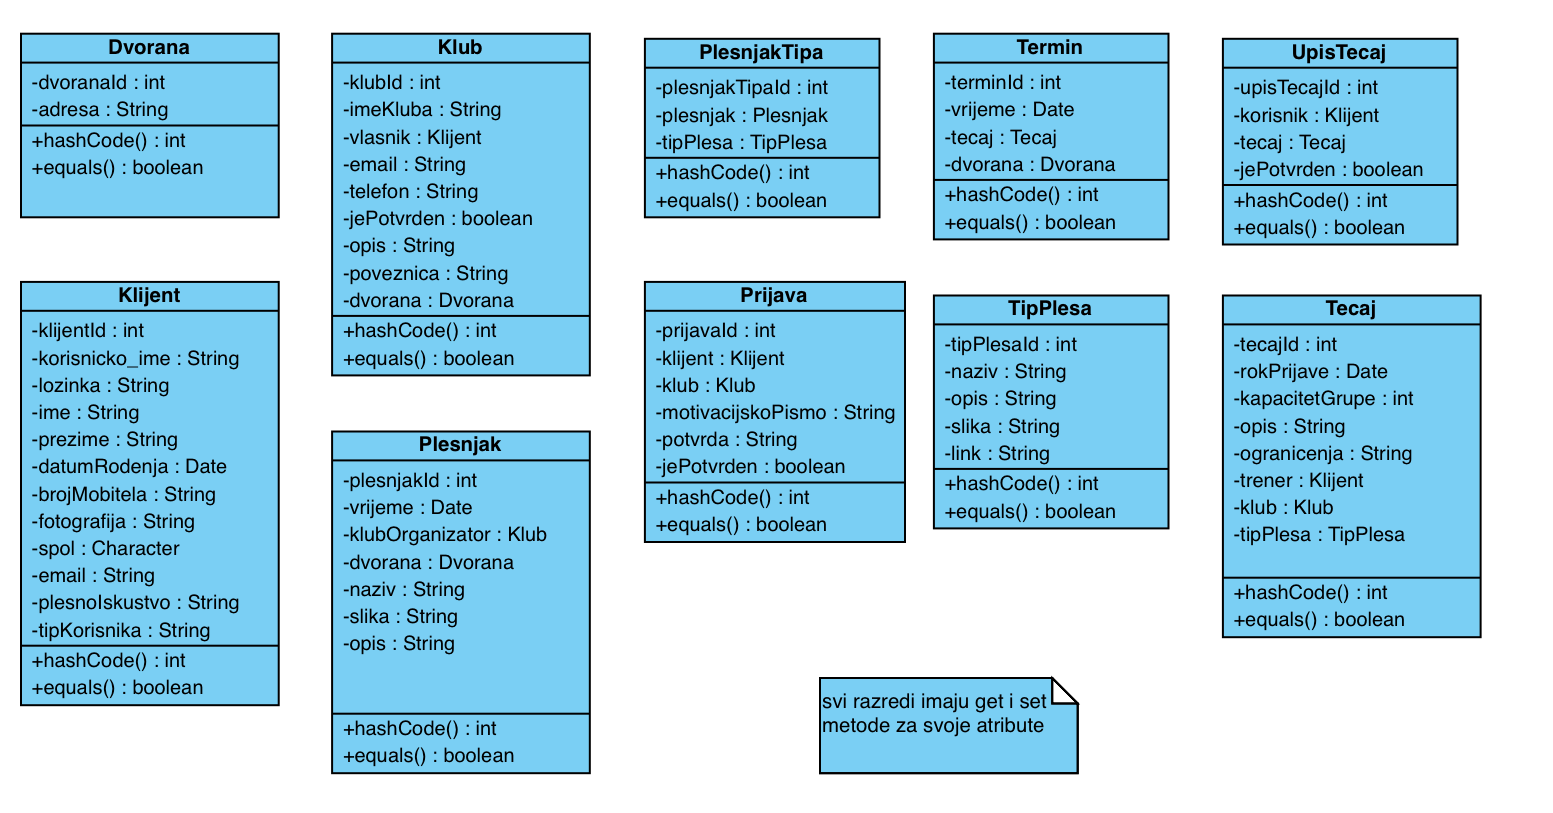
\includegraphics[width=\textwidth]{slike/dijagram_razreda/model.png}
				\caption{Dijagram razreda (Model)}
				\label{fig:my_label}
		    \end{figure}
	    	
	    	\begin{figure}[H]
	    		\centering
	    		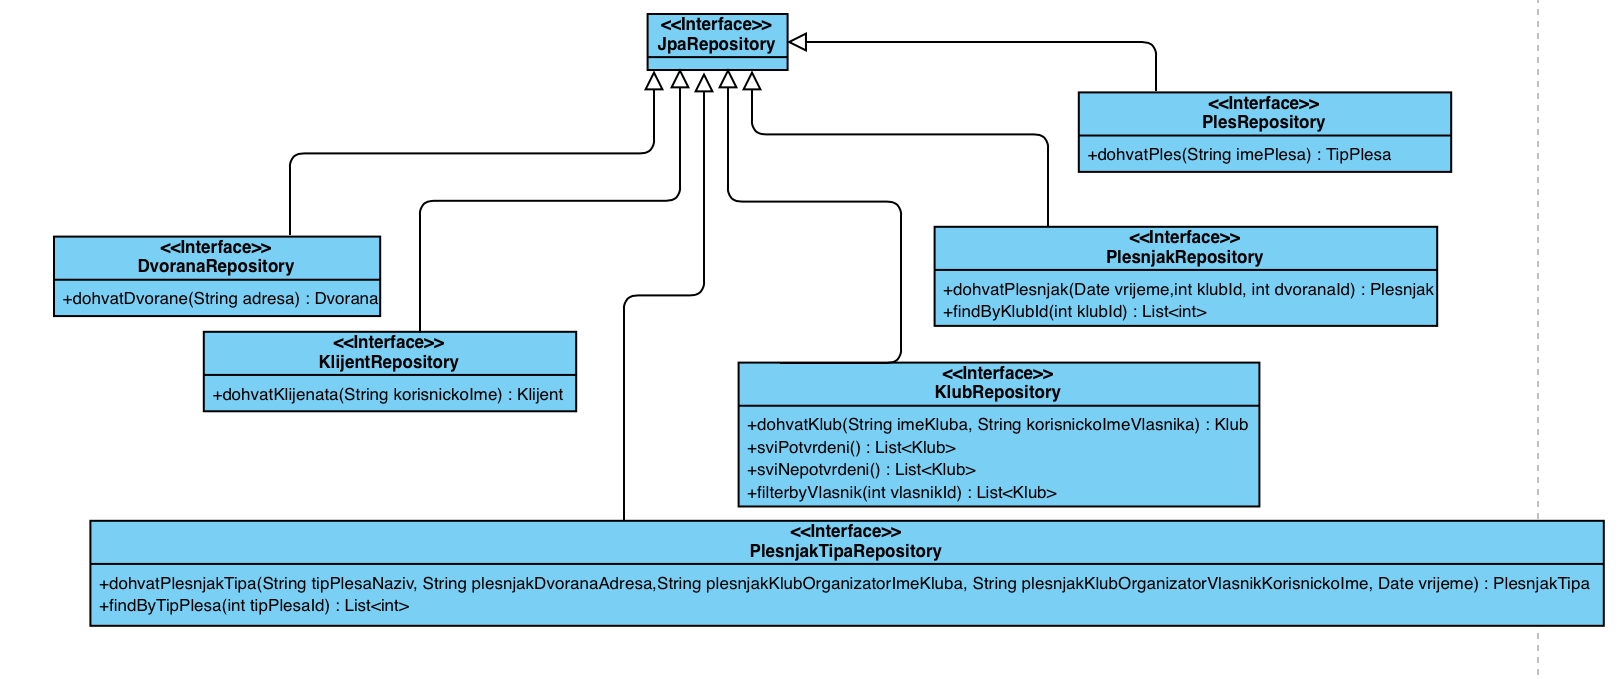
\includegraphics[width=\textwidth]{slike/dijagram_razreda/repository.png}
	    		\caption{Dijagram razreda (Repository)}
	    		\label{fig:my_label}
	    	\end{figure}
    	
    	\begin{figure}[H]
    		\centering
    		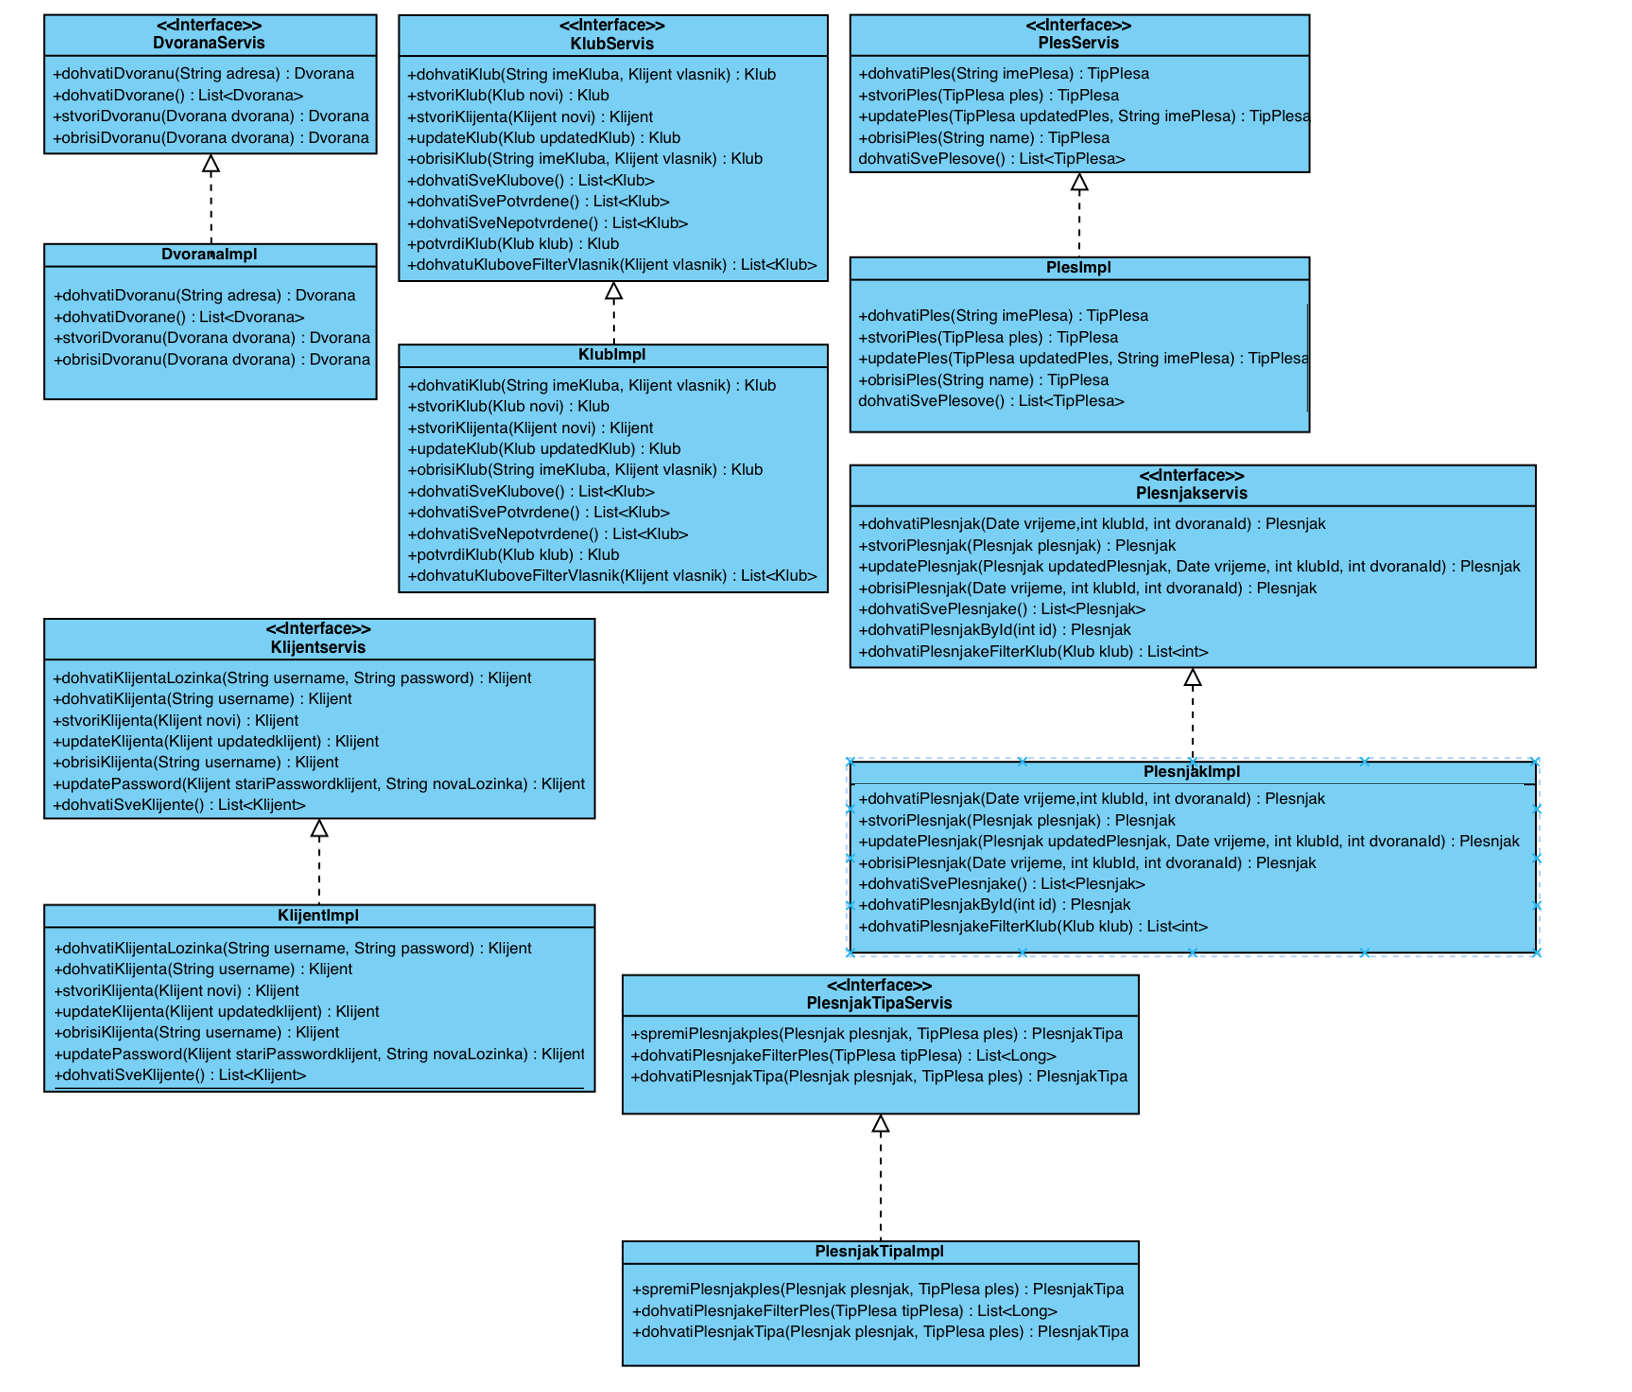
\includegraphics[width=\textwidth]{slike/dijagram_razreda/service.png}
    		\caption{Dijagram razreda (Service)}
    		\label{fig:my_label}
    	\end{figure}
    	
    	\begin{figure}[H]
    		\centering
    		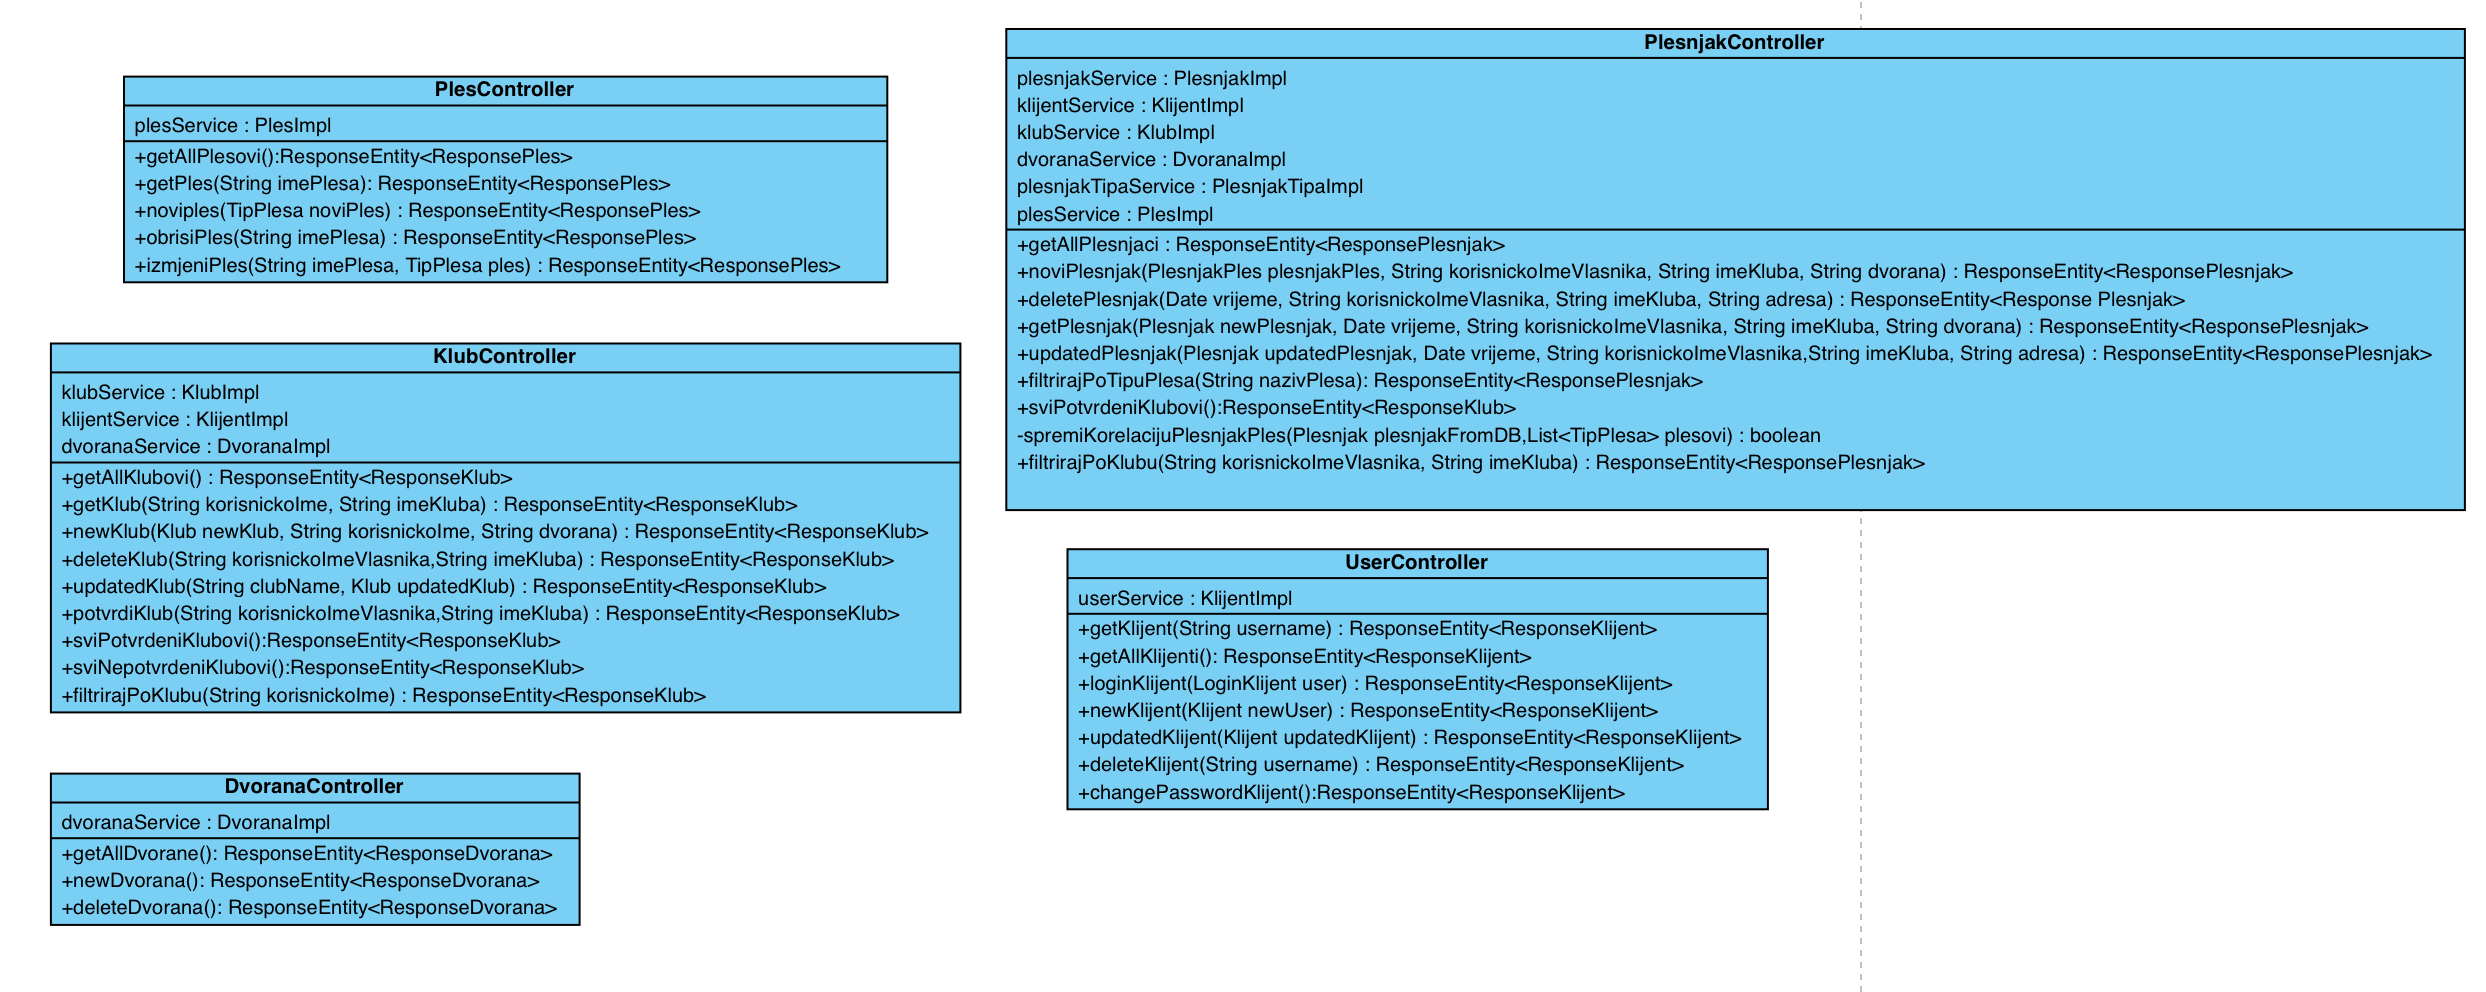
\includegraphics[width=\textwidth]{slike/dijagram_razreda/controller.png}
    		\caption{Dijagram razreda (Controller)}
    		\label{fig:my_label}
    	\end{figure}
			
	
			
			\section{Dijagram stanja}
			
			\textit{ Dijagram stanja prikazuje stanja objekta te prijelaze iz jednog stanja u drugo temeljene na događajima. Prilikom pokretanja aplikacije dolazi se na početnu stranicu (eng.Home page). Neregistrirani korisnik ima mogućnost registracije/prijave u sustav ili može ostati neregistriran. \linebreak \textbf{Slika 4.9} prikazuje dijagram stanja za registriranog korisnika. Nakon prijave, klijentu se prikazuje početna stranica na kojoj je karta s dostupnim plesnjacima i lokacijama klubova. Klikom na karticu „Profile“  klijentu je dostupan pregled profila. Klijent može pregledati, mijenjati osobne podatke i izbrisati korisnički račun. Odabirom kartice „My Clubs“ klijentu se pruža mogućnost registracije vlastitog kluba. Novo registrirani klubovi prvo moraju biti potvrđeni od strane administratora. Klikom na lokaciju kluba na karti otvara se profil kluba. Na stranici "profil kluba" korisnik može pregledati sve klubove, tečajeve, uređivati podatke ili izbrisati klub. Također može organizirati plesnjak ili postati trenerom za što postoje odgovarajuće forme. Ako je korisnik administrator onda može klikom na karticu "Admin" pregledati sve klijente, plesove i klubove. Može organizirati plesnjak, napraviti listu plesova te potvrđivati novonastale klubove.}
			
			\begin{figure}[H]
				\centering
				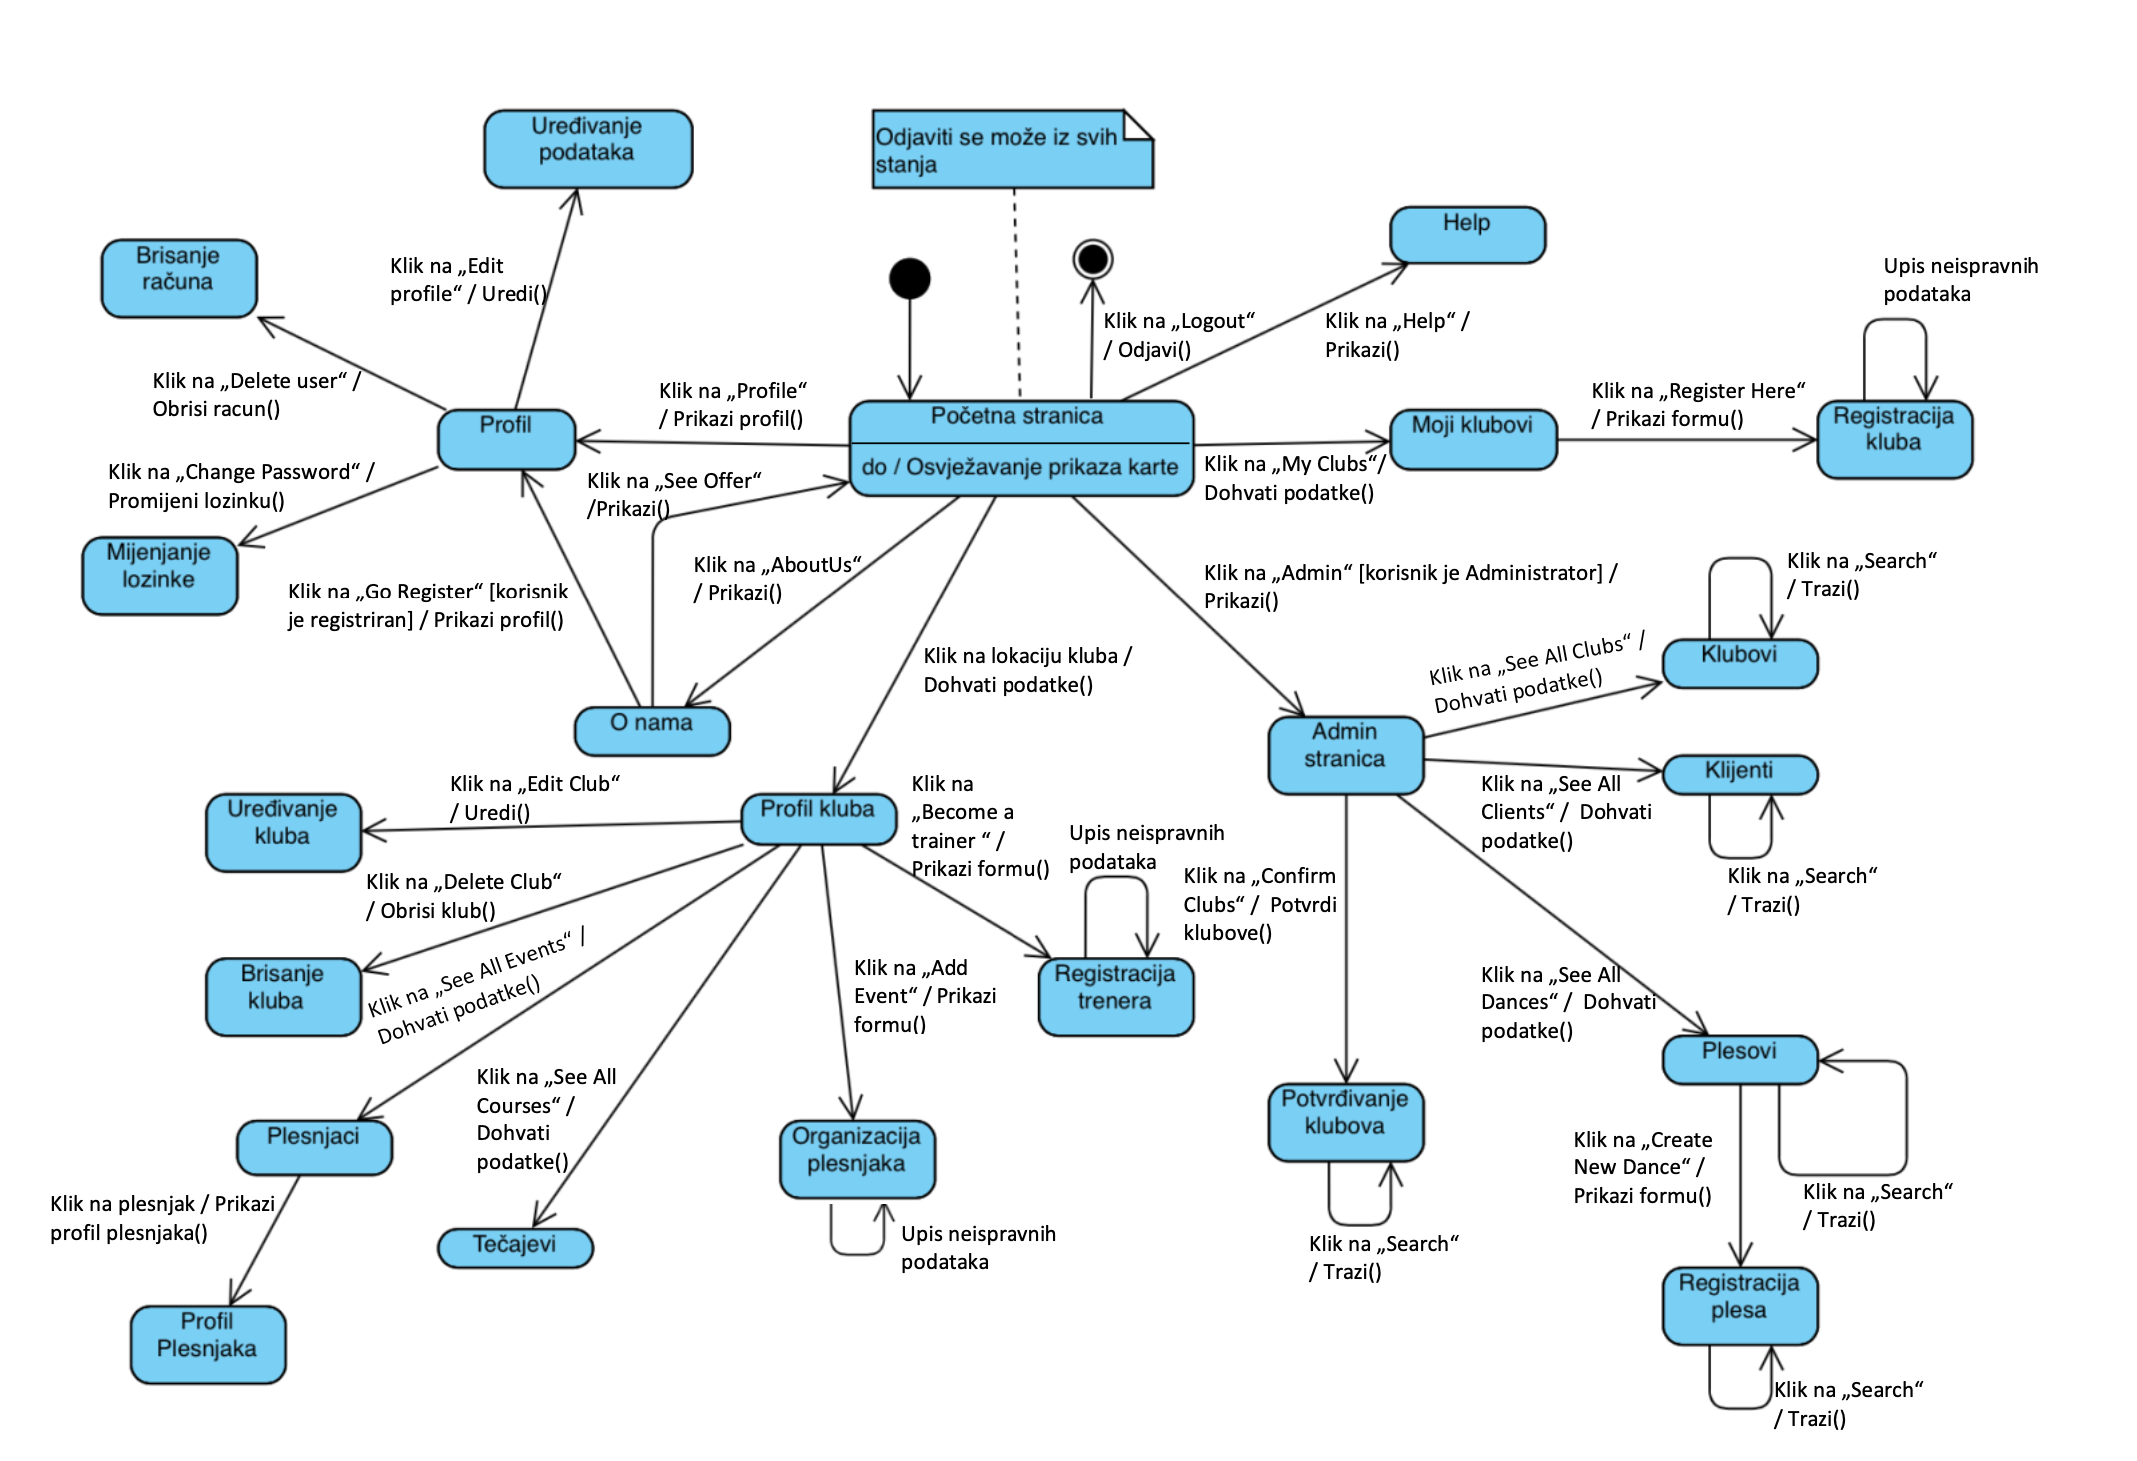
\includegraphics[width=\textwidth]{slike/dijagram_stanja.png}
				\caption{Dijagram stanja (Klijent)}
				\label{fig:my_label}
		   	\end{figure}
			
		
			
			\section{Dijagram aktivnosti}
	
			\textit{Dijagram aktivnosti opisuje model toka upravljanja ili toka podataka. Svaki novi korak obavlja se nakon završenog prethodnog. Slika 4.10 prikazuje dijagram aktivnosti za proces organizacije/stvaranja  plesnjaka. Korisnik se prijavi u sustav te mu se na početnoj stranici prikaže karta s klubovima. Odabire jedan klub za koji će stvoriti plesnjak. Otvara se stranica odabranog kluba na kojoj se pruža mogužnost stvaranja plesnjaka. Kada korisnik  upiše odgovarajuće podatke, na stranici profila kluba nalazi se lista novostvorenih plesnjaka. }
			
			\begin{figure}[H]
			\centering
			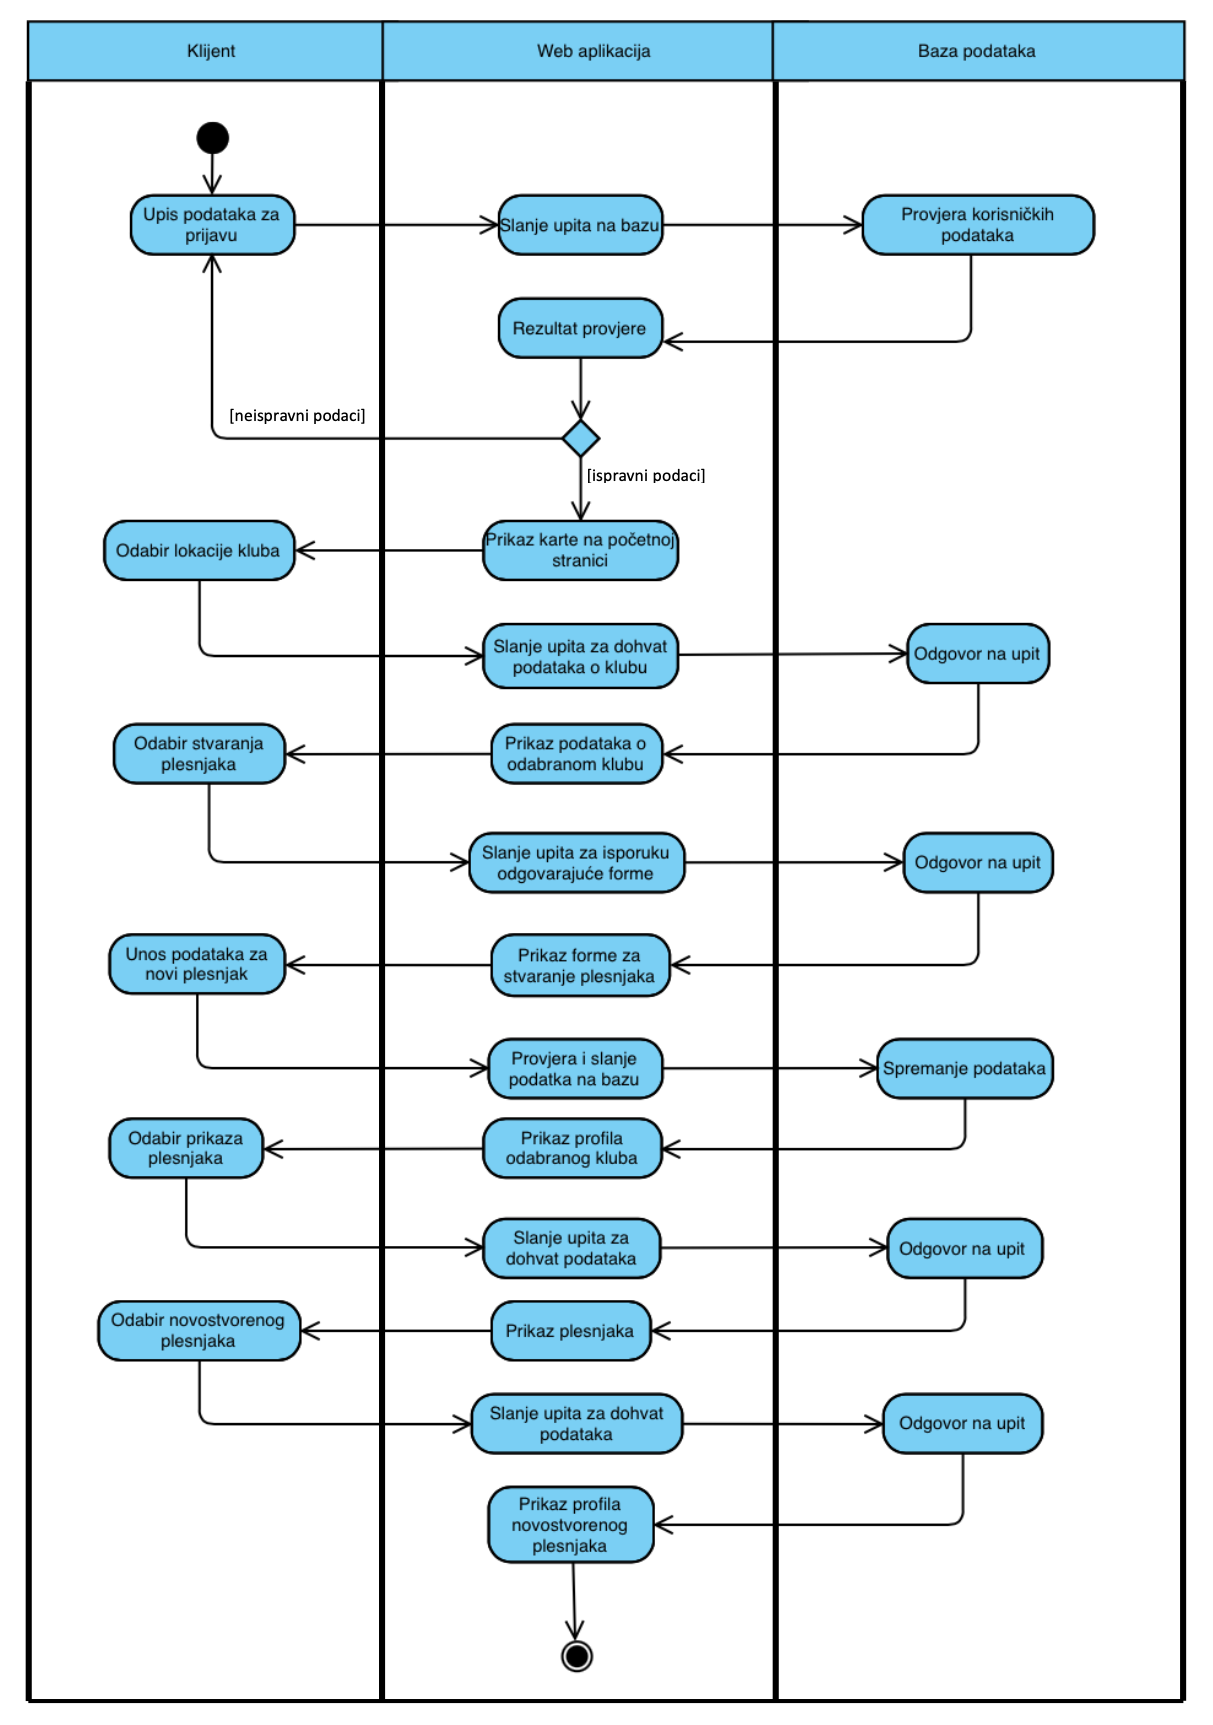
\includegraphics[width=\textwidth]{slike/dijagram_aktivnosti.png}
			\caption{Dijagram aktivnosti(Organizacija plesnjaka)}
			\label{fig:my_label}
	     	\end{figure}
	 	\eject 
			
			
			\section{Dijagram komponenti}
			\textit{Dijagram komponenti opisuje organizaciju i međuovisnost komponenti, interne strukture i odnose prema okolini. Prikazan je kao frontend i backend aplikacija koje su integrirane REST API-jem.}
			
			\textit{Backend aplikacija sastoji se od modela, servisa, repozitorija i kontrolera. Model nam služi za organizaciju podataka koji će se spremati u bazu. Repozitorij komunicira s bazom podataka (SQL upiti) za dohvaćanje podataka koji su nam potrebni. Servis komunicira sa repozitorijem i kontrolerom. Kontroler obrađuje dolazne zahtjev (zahtjeve sa frontenda). }
			\textit{Frontend aplikacija se sastoji od routera, komponenti, servisa te raznih biblioteka. Router je komponenta koja na korisnikov upit za određeni url određuje koja će se datoteka (stranica) isporučiti. Komponente su stranice koje se isporučuju odnosno to su javascript datoteke (html, css, javascript kod) koje ovise o React biblioteci.  Servisi nam ovdje služe za pozive prema backendu, validacije i slično. Axios je biblioteka HTTP klijenta koja olakšava slanje HTTP zahtjeva na REST API (odnosno slanje zahtjeva na backend aplikaciju). }
		
		
			\begin{figure}[H]
				\centering
				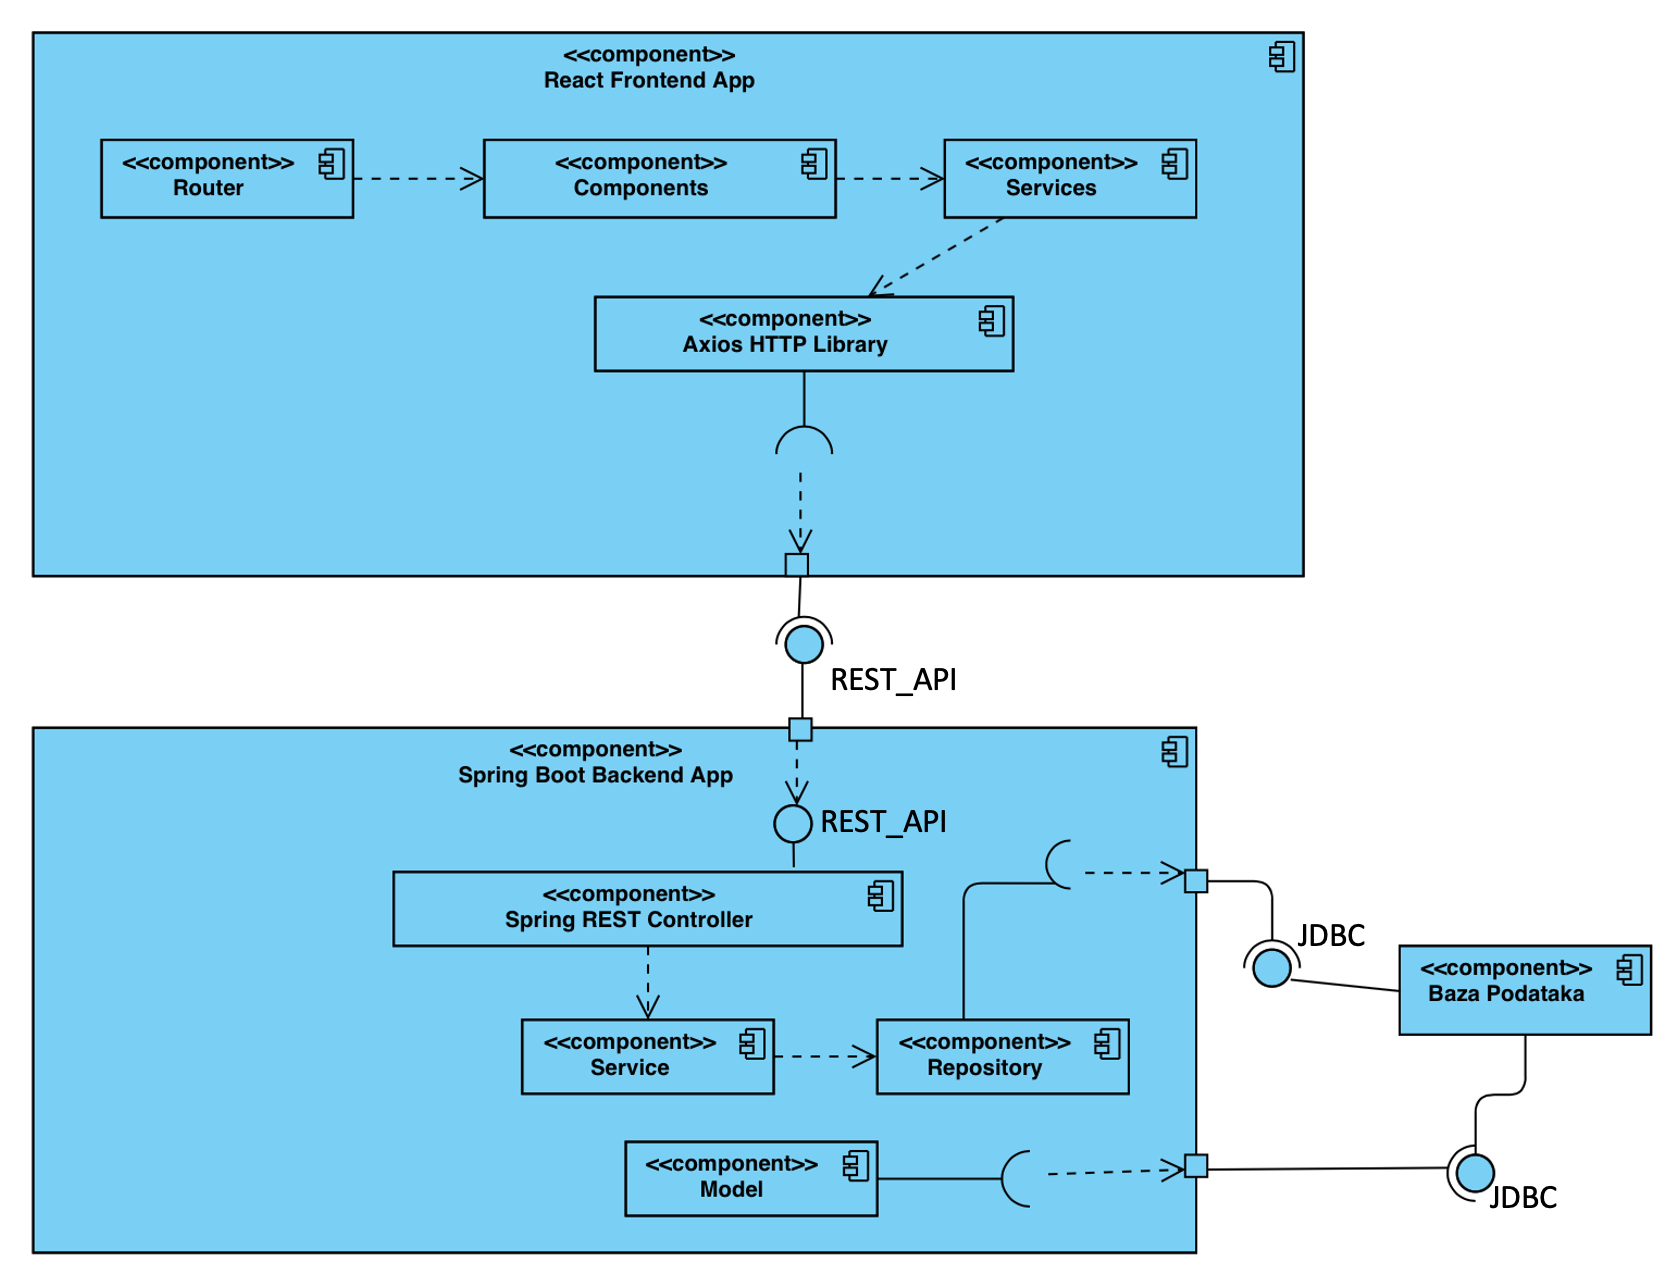
\includegraphics[width=\textwidth]{slike/dijagram_komponenti.png}
				\caption{Dijagram komponenti}
				\label{fig:my_label}
			\end{figure}
			
			
			
			
			
	\chapter{Implementacija i korisničko sučelje}
		
		
		\section{Korištene tehnologije i alati}
		\bigskip
			
		\textbf{\textit{izrada aplikacije}}
		\bigskip
		\bigskip
		
			 \textit{ Po modelu klijent - poslužitelj, "klijentska strana aplikacije" (front-end) realizirana je pomoću Reacta\footnote{\url{https://reactjs.org}} u razvojnom okruženju Visual Studio Code\footnote{\url{https://code.visualstudio.com}} uz korištenje jezika Javascript\footnote{\url{https://www.javascript.com}} .  React je Javascript biblioteka otvorenog koda za izgradnju korisničkih sučelja temeljenih na komponentama korisničkog sučelja. Za implementaciju "poslužiteljske strane" (back-enda) korišten je Spring Boot\footnote{\url{https://spring.io/projects/spring-boot}} zasnovan na razvojnom okviru Spring\footnote{\url{https://spring.io}} u razvojnom okruženju Eclipse\footnote{\url{https://www.eclipse.org}} uz korištenje jezika Java\footnote{\url{https://www.java.com/en/}} . Arhitektura sustava je oblikovana objektno usmjereno pa iz tog razloga koristimo Javu kao objektno orijentirani programski jezik. Spring Boot je radni okvir temeljen na Javi. Za prikladno strukturiranje i spremanje podatka korištena je relacijska baza podataka, implementirana pomoću PostgreSQL-a\footnote{\url{https://commandprompt.com/education/how-to-download-and-install-postgresql/}} . Relacijska baza podataka nam osigurava laku manipulaciju podacima te određenu razinu sigurnosti.}
			 
		\bigskip
			\bigskip
			 
			 \textbf{\textit{izrada dokumentacije}}
			 \bigskip
			 

    				 \textit{Za izradu dokumentacije korišten je markup jezik LaTeX\footnote{\url{https://www.latex-project.org}} (slično kao HTML). LaTeX datoteka je tip tekstualne datoteke koja nam olakšava rad sa sustavom za verzioniranje. Korišten je TeXstudio\footnote{\url{https://www.texstudio.org/}}, uređivač teksta koji je prilagođen LaTeXu. Za kreiranje pdf dokumenta iz LaTeX dokumenta korišten je TeXLive\footnote{\url{https://www.tug.org/texlive/}} . Za izradu UML dijagrama korišten je online alat VisualParadigm\footnote{\url{https://online.visual-paradigm.com/drive/\#diagramlist:proj=0&dashboard}}. }
				 \bigskip
			 
			 \textbf{\textit{ostalo}}
			 \bigskip
			 
				 \textit{	Komunikacija u timu realizirana je korištenjem aplikacije WhatsApp\footnote{\url{https://www.whatsapp.com}} i Discord\footnote{\url{https://discord.com}}. Kao sustav za upravljanje izvornim kodom korišten je Git\footnote{\url{https://git-scm.com/}} . Udaljeni repozitorij projekta dostupan je na web platformi GitLab \footnote{\url{https://gitlab.com/}} .}
			 	
		\newpage
		\section{Ispitivanje programskog rješenja}

			
			 \textit{Za testiranje funkcionalnosti komponenti i sustava korišteni su Selenium WebDriver i Selenium IDE ekstenzija za Chrome preglednik. }
	
			
			\subsection{Ispitivanje komponenti}
			\textit{Na slikama 5.1,5.2 i 5.3 prikazani su unit testovi uz korištenje Selenium WebDriver podrške.  Slika 5.4 omogućava uvid u uspješnost izvršavanja testova.}
		\newline
		\newline
			\textit{Na slici 5.1 možemo vidjeti testiranje metode dohvatiKlijenta iz implementacije klijent servisa i uspješno dohvaćanje korisnika. }
			\begin{figure}[H]
				\centering
				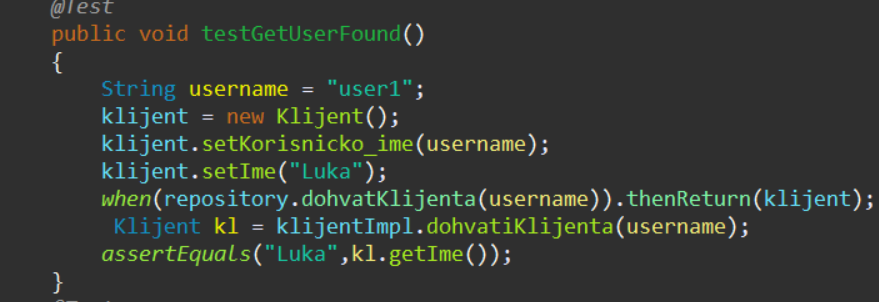
\includegraphics[width=\textwidth,height=8cm]{slike/slike_testova/JUNIT/test1.PNG}
				\caption{Dohvaćanje postojećeg korisnika}
				\label{fig:my_label}
			\end{figure}
		
		
		\newpage
		
		\textit{
			Slika 5.2 prikazuje pokušaj dohvaćanja klijenta koji nije u repozitoriju što vraća null vrijednost. }
		\begin{figure}[H]
			\centering
			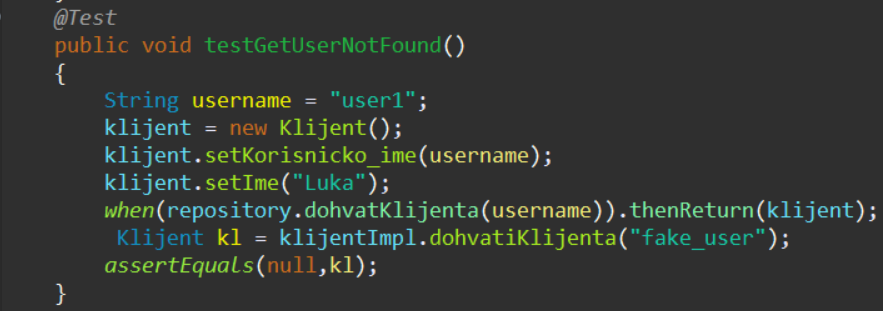
\includegraphics[width=\textwidth,height=8cm]{slike/slike_testova/JUNIT/test2.PNG}
			\caption{Dohvaćanje nepostojećeg korisnika}
			\label{fig:my_label}
		\end{figure}
	
	\textit{
		Slika 5.3 prikazuje slučaj brisanja korisnika koji nije prethodno dodan u repozitorij i stoga brisanje nije moguće. Povratna vrijednost metode je null. }
	\begin{figure}[H]
		\centering
		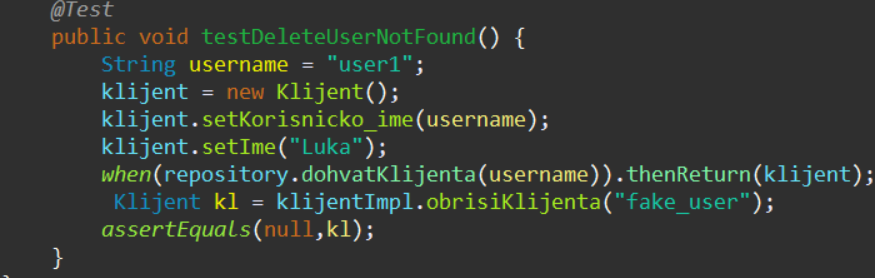
\includegraphics[width=\textwidth,height=8cm]{slike/slike_testova/JUNIT/test3.PNG}
		\caption{Brisanje nepostojećeg korisnika}
		\label{fig:my_label}
	\end{figure}
			
			\newpage
			\begin{figure}[H]
				\centering
				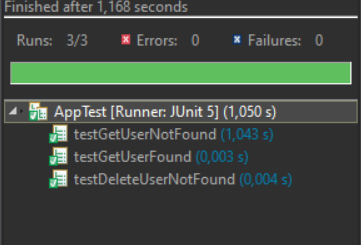
\includegraphics[width=\textwidth,height=8cm]{slike/slike_testova/JUNIT/results.PNG}
				\caption{Rezultati JUNIT testova}
				\label{fig:my_label}
			\end{figure}
			
			\subsection{Ispitivanje sustava}
			
			 \textit{Na slikama 5.5 do 5.11 prikazano je testiranje sustava i rezultati dobiveni korištenjem Selenium IDE. }
			 
			\newline
			\textit{
				Slika 5.5 prikazuje pokušaj izrade kluba koji već postoji. }
			\begin{figure}[H]
				\centering
				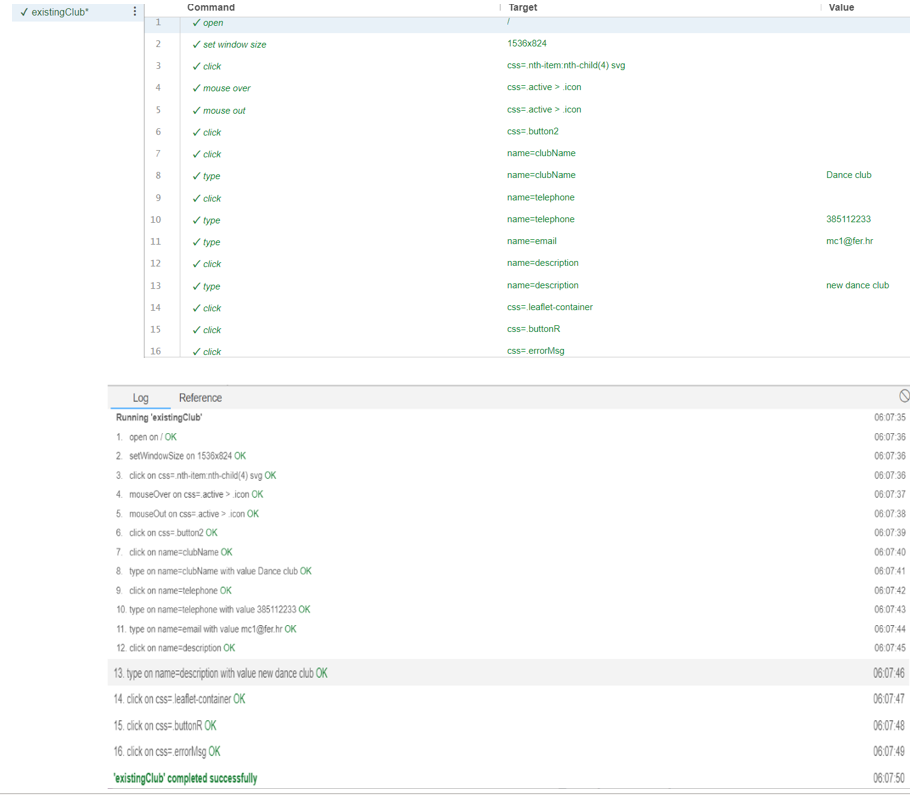
\includegraphics[width=\textwidth,height=8.5cm]{slike/slike_testova/SELENIUM_IDE/1.PNG}
				\caption{Kreiranje postojećeg kluba}
				\label{fig:my_label}
			\end{figure}
		\newpage
		\textit{
			Slika 5.6 prikazuje pokušaj prijave korisnika za instruktora plesa bez priloženih trenerskih akreditiva. }
		\begin{figure}[H]
			\centering
			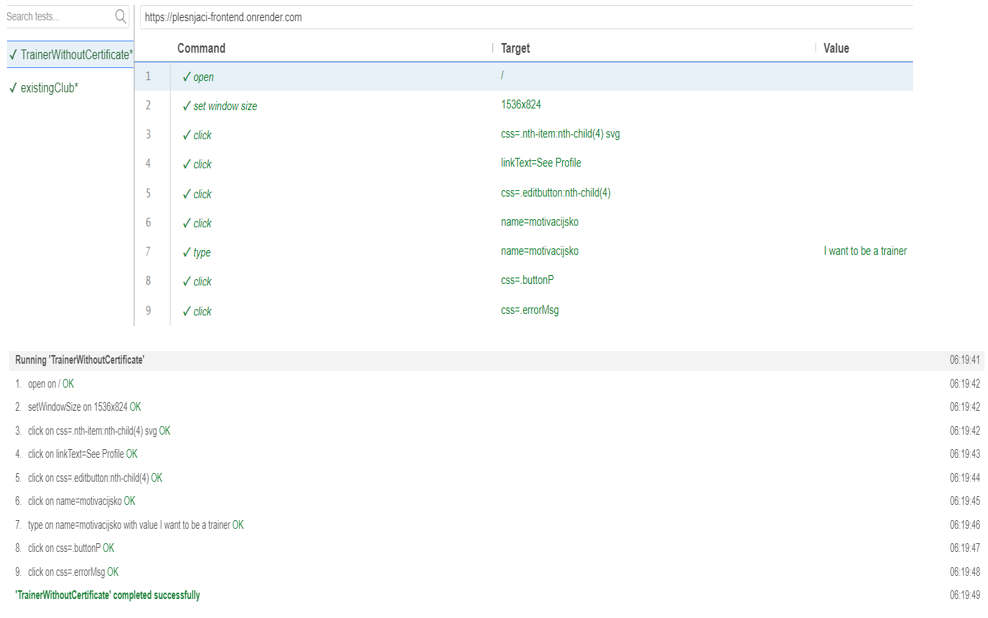
\includegraphics[width=\textwidth,height=8.5cm]{slike/slike_testova/SELENIUM_IDE/2.PNG}
			\caption{Pokušaj prijave za instruktora}
			\label{fig:my_label}
		\end{figure}
	\textit{
		Na slici 5.7 vidimo pokušaj registracije korisnika koji već postoji u sustavu i stoga nije moguć. }
	\begin{figure}[H]
		\centering
		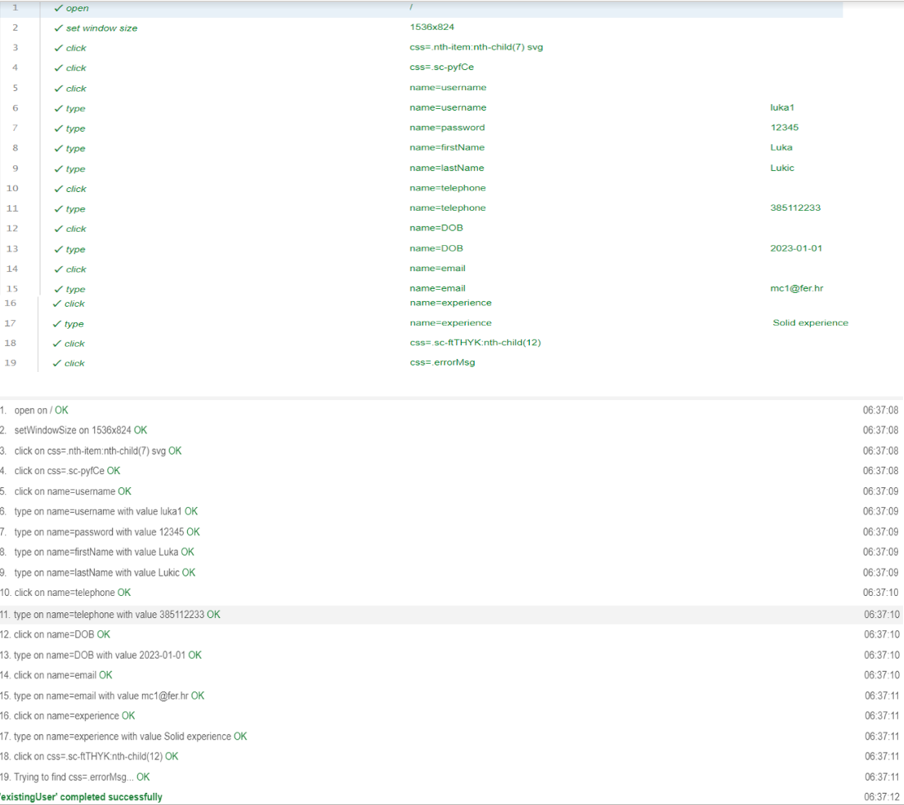
\includegraphics[width=\textwidth,height=8cm]{slike/slike_testova/SELENIUM_IDE/3.PNG}
		\caption{Nedozvoljeni pokušaj registracije}
		\label{fig:my_label}
	\end{figure}
	\newpage
	\textit{
		Slika 5.8 pokazuje pokušaj izrade tečaja bez specificiranja o kojoj vrsti plesa se radi što nije dozvoljeno. }
	\begin{figure}[H]
		\centering
		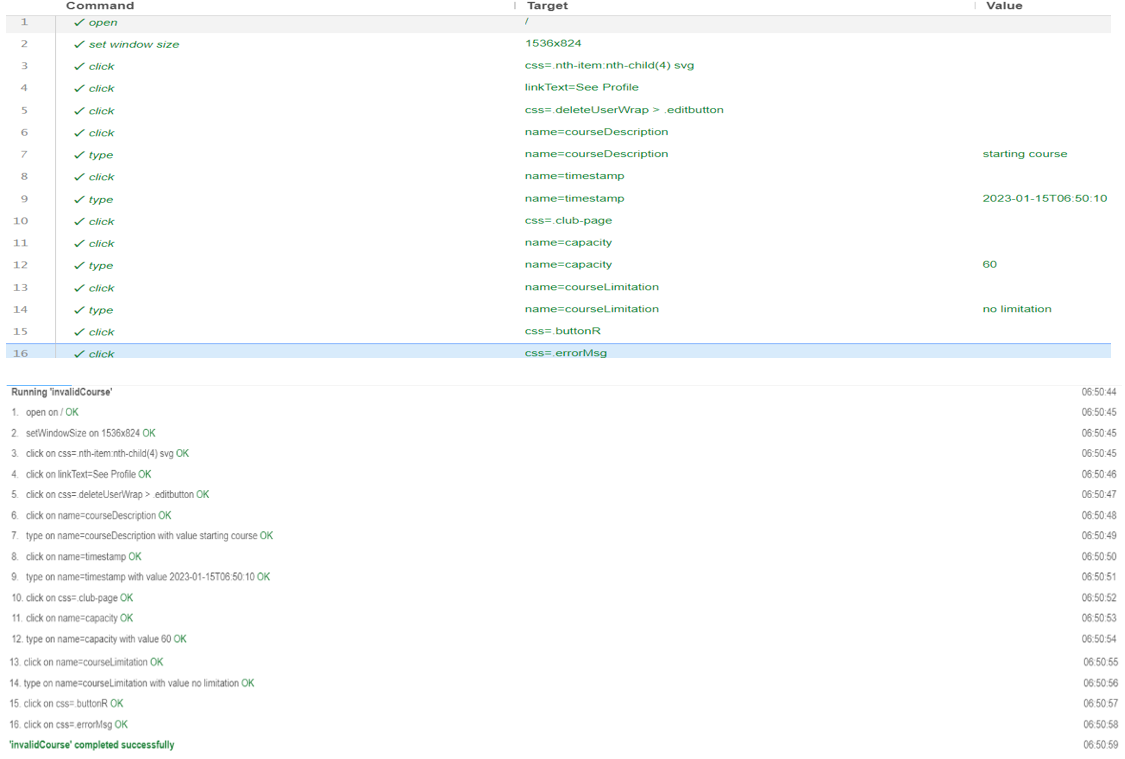
\includegraphics[width=\textwidth,height=8cm]{slike/slike_testova/SELENIUM_IDE/4.PNG}
		\caption{Nedozvoljeno kreiranje tečaja}
		\label{fig:my_label}
	\end{figure}
\textit{
	Slika 5.9 prikazuje pokušaj izmjene događaja uz navođenje neispravnog formata datuma što uzrokuje grešku. }
\begin{figure}[H]
	\centering
	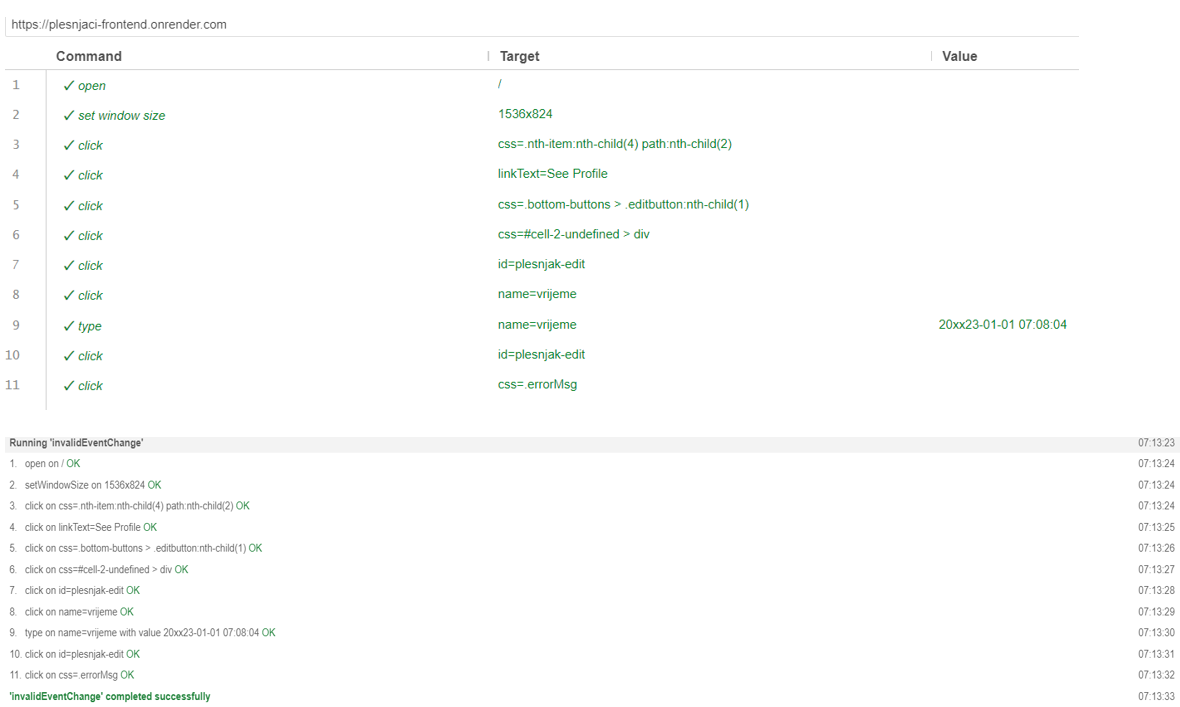
\includegraphics[width=\textwidth,height=8cm]{slike/slike_testova/SELENIUM_IDE/5.PNG}
	\caption{Nepravilna izmjena datuma}
	\label{fig:my_label}
\end{figure}
\newpage
	\textit{
		Na slici 5.10 prikazano je ispravno brisanje korisnika uz potvrdu. }
	\begin{figure}[H]
		\centering
		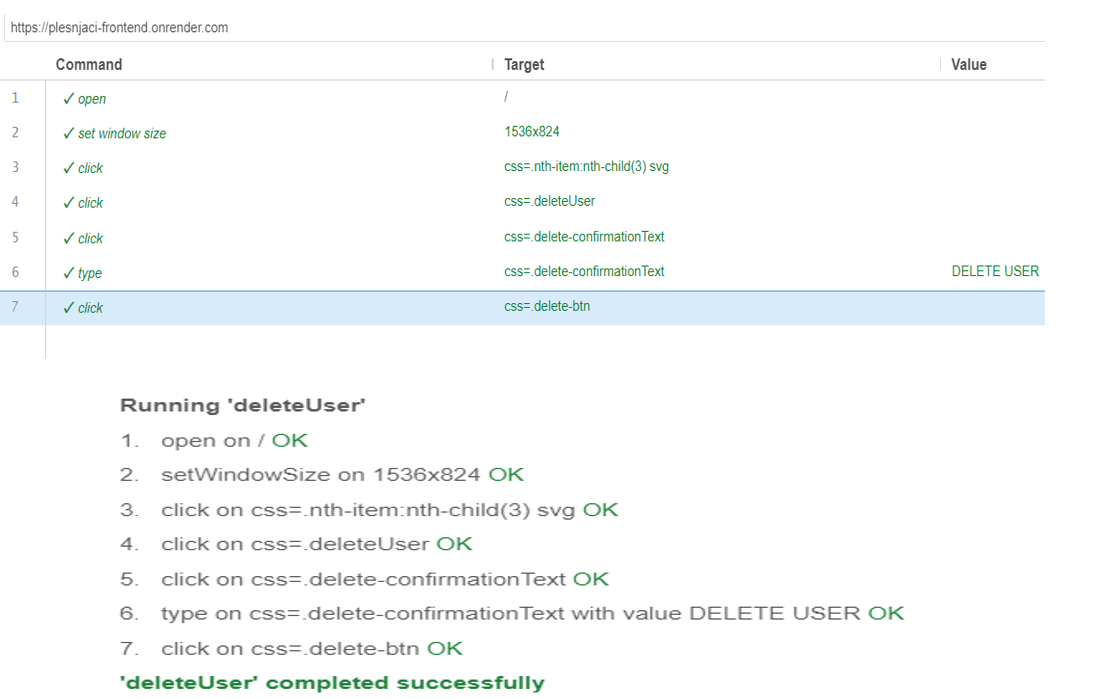
\includegraphics[width=\textwidth,height=8cm]{slike/slike_testova/SELENIUM_IDE/6.PNG}
		\caption{Ispravno brisanje korisnika}
		\label{fig:my_label}
	\end{figure}
\textit{
	Slika 5.11 sadržava pokušaj registracije korisnika uz unošenje nedozvoljenog tipa informacija. }
\begin{figure}[H]
	\centering
	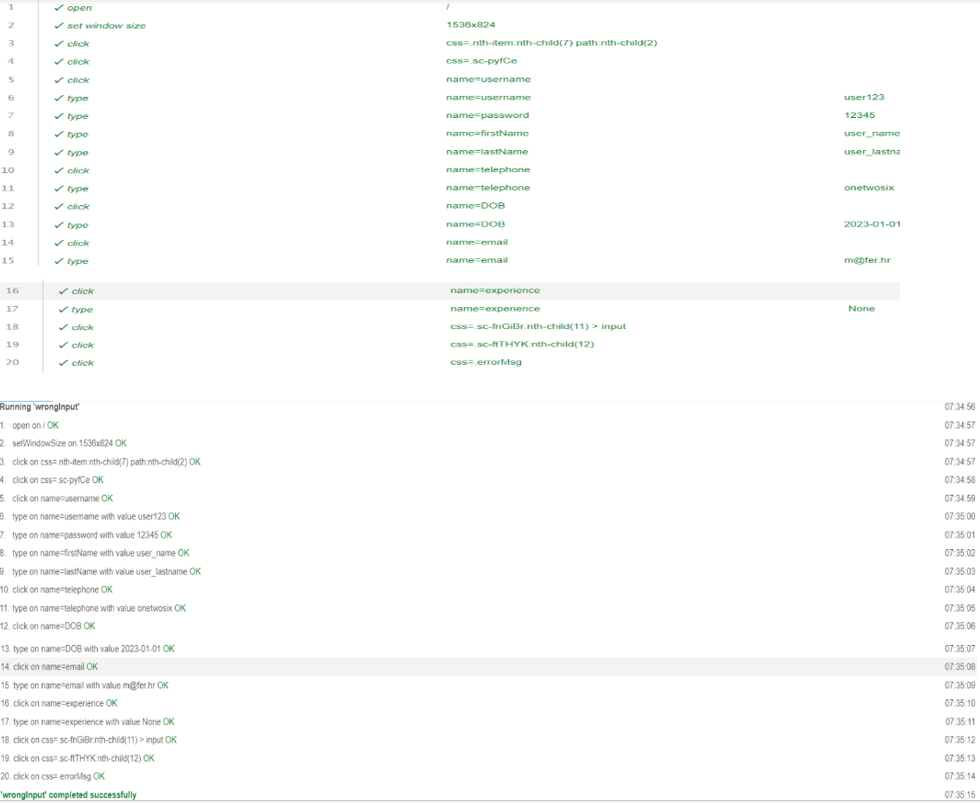
\includegraphics[width=\textwidth,height=9.5cm]{slike/slike_testova/SELENIUM_IDE/7.PNG}
	\caption{Nedozvoljen tip podataka}
	\label{fig:my_label}
\end{figure}
			\eject 
		
		
		\section{Dijagram razmještaja}
		\bigskip
		\bigskip
		
			\textit{Dijagram razmještaja opisuje topologiju sustava, odnos sklopovskih i programskih dijelova. Slika 5.1 prikazuje specifikacijski dijagram razmještaja. Na poslužiteljskom računalu nalazi se web aplikacija i baza podataka. Klijenti koriste web preglednik kako bi pristupili aplikaciji. Sustav funkcionira po modelu "klijent - poslužitelj". Klijent zahtjeva uslugu od strane poslužitelja, šalje mu HTTP zahtjev i očekuje odgovor. Poslužitelj obrađuje zahtjeve te šalje odgovor klijentu. Poslužitelj je također zadužen za komunikaciju s bazom podataka. }

			\bigskip
			\bigskip
			
			\begin{figure}[H]
				\centering
				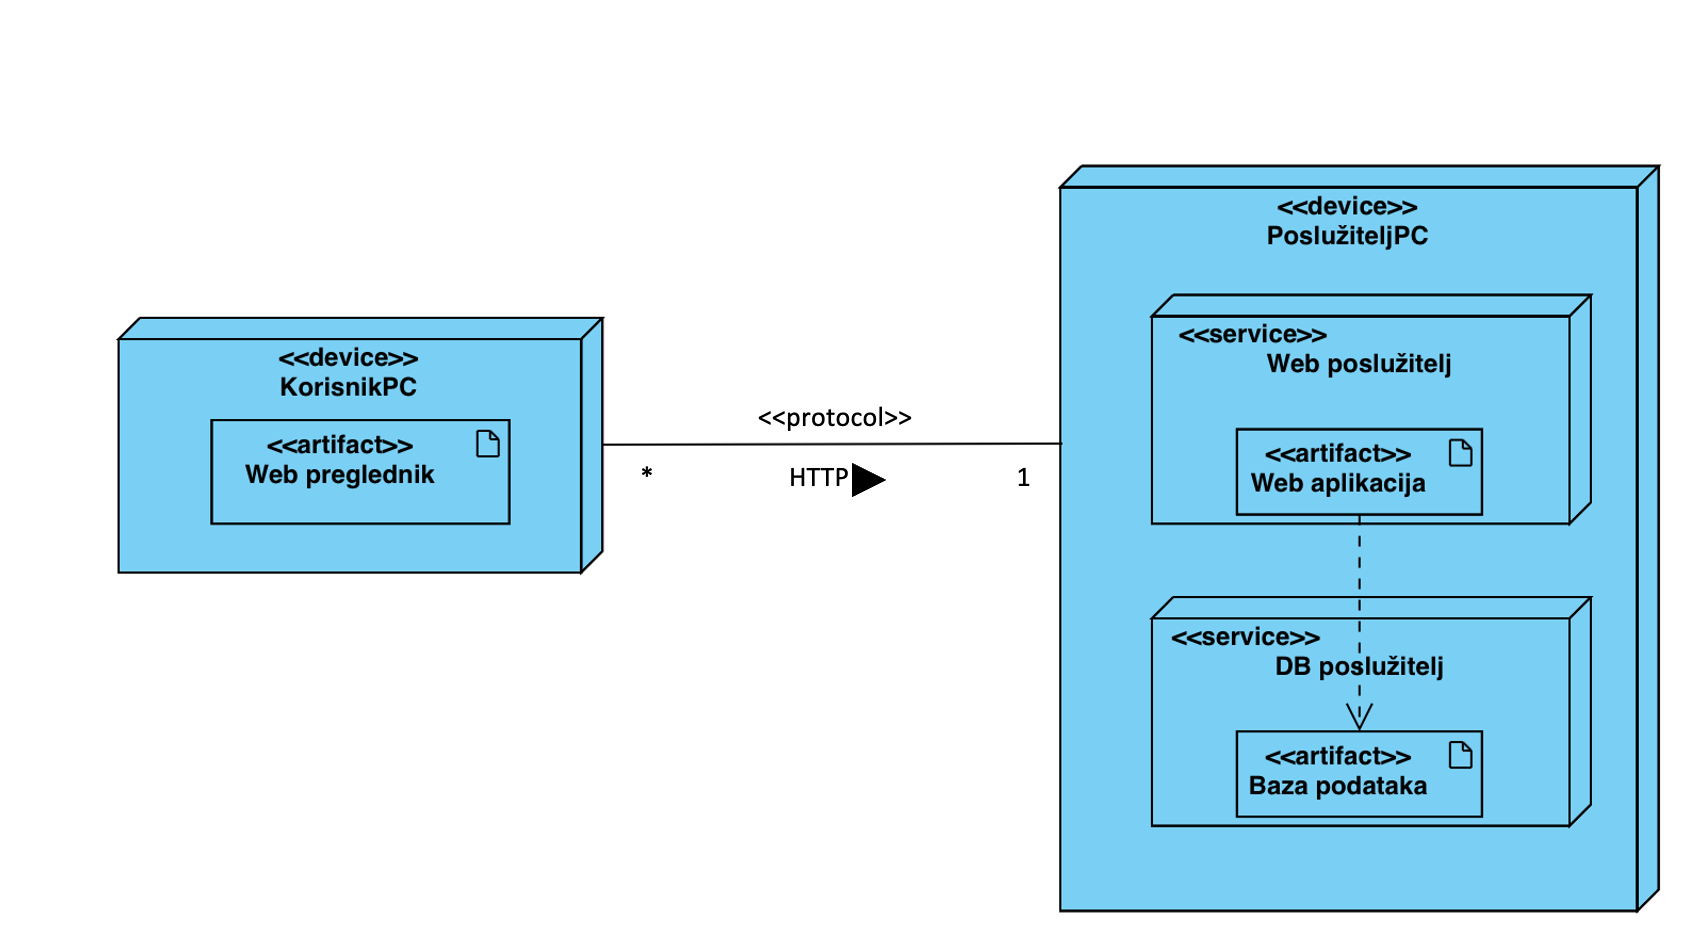
\includegraphics[width=\textwidth]{slike/dijagram_razmjestaja.png}
				\caption{Specifikacijski dijagram razmještaja}
				\label{fig:my_label}
			\end{figure}
		
		
		\newpage
		
		
		\section{Upute za puštanje u pogon}
		
		\textbf{\textit{Općenito}}\\
			\textit{Za puštanje aplikacije u pogon koristili smo Render cloud servis za hostanje baze podatka te backend i frontend aplikacija. Odabrali smo Render zato što pruža mogućnost automatske izgradnje aplikacije svaki put kad se dogodi promjena u samom kodu aplikacije. Kod je spremljen u master grani povezanog GitLab repozitorija. Ako se promjena dogodi na frontend aplikaciji samo će se ona ponovno izgraditi, a backend aplikacija zbog toga neće prestati s radom. Preko Render Dashboard-a moguće je vidjeti konzolu za pojedinu aplikaciju. Kako bi vidjeli trenutno stanje baze podataka na nju se spajamo pomoću pgAdmin-a (potrebno je instalirati windows aplikaciju).
			Prvi korak za puštanje aplikacije u pogon je registracija na Render web stranici \footnote{\url{render.com}}. Prilikom registracije, Render korisnički račun potrebno je povezati s GitLab korisničkim računom koji pripada određenom studentu iz grupe kako bi se omogućio pristup GitLab repozitoriju. Nakon što je registracija dovršena vidjet će se Render Dashboard na kojem se mogu vidjeti sve aplikacije i baze podataka koje su povezane s tim korisničkim računom.}
		\bigskip
	
		\textbf{\textit{Stvaranje baze podataka}}\\
			\textit{Na Render Dashboardu potrebno je kliknuti na „New“ pa zatim odabrati „PostgreSQL“ kako bi započeo proces stvaranje baze podataka. Na formi za stvaranje baze podataka potrebno je u polje „Database“ upisati željeno ime baze podataka, „Region“ treba postaviti na „Frankfurt“, „PostgreSQL Version“ na „15“ i „Instance Type“ na „Free“. Polje „Name“ će biti ime baze podataka koje će pisati na Render Dashboard-u(ne mora biti isto kao pravo ime baze podataka), polja „User“(ime vlasnika baze podataka) i „Datadog API Key“ su opcionalna, a lozinka baze podataka će biti automatski generirana prilikom stvaranja baze. Nakon što su podaci uneseni u formu baza podataka se stvara pritiskom na gumb „Create Database“. Odabirom novo stvorene baze podataka na Render Dashboard-u prikazat će se informacije o bazi podataka. Slika 5.2 prikazuje neke bitne informacije o bazi podataka do kojih se može doći odabirom na „Info“ pa spuštanjem do sekcije „Connections“. Neki od ovih podataka koristit će se kao environment varijable(objašnjeno kasnije) u backend aplikaciji.}
		\bigskip
	
		\begin{figure}[H]
		\centering
		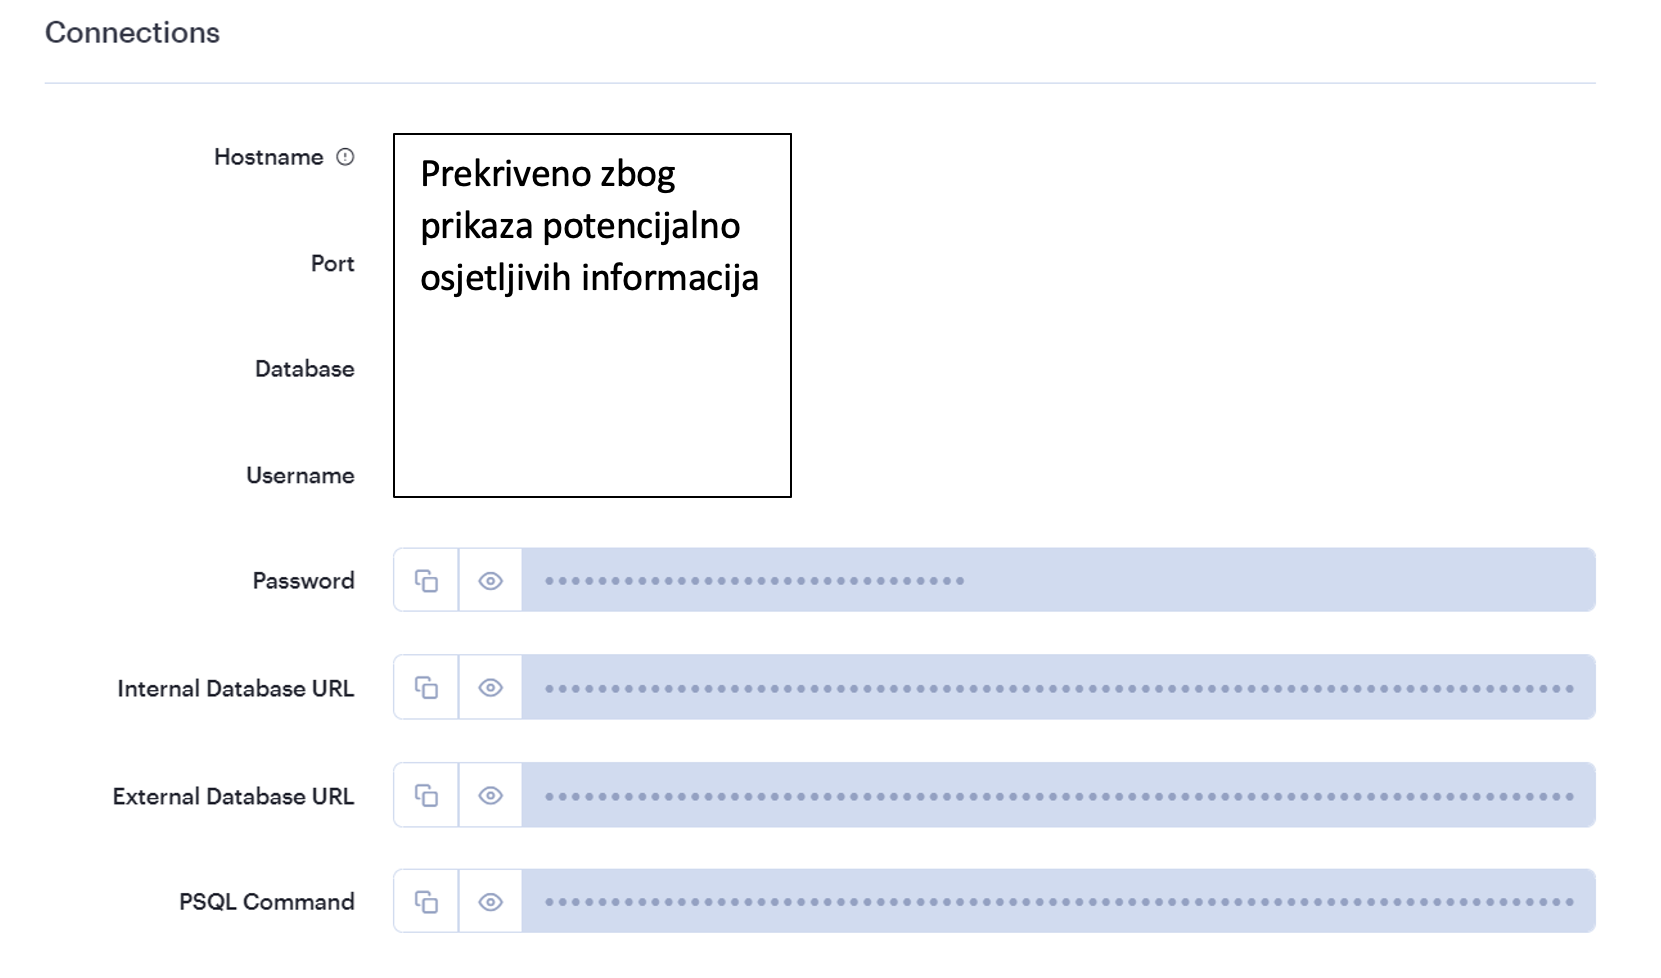
\includegraphics[width=\textwidth]{slike/deployment/slika1.png}
		\caption{Informacije o bazi na Render-u}
		\label{fig:my_label}
    	\end{figure}
    
    \bigskip
    
    	\textbf{\textit{Spajanje pg-Admina s bazom podataka}}\\
		    \textit{Nakon što se instalira pgAdmin potrebno ga je pokrenuti te zatim odabrati opciju „Object“ pa „Register“ pa „Server“ da bi se pojavila forma za spajanje na novu bazu podataka. Prvo,  u polje „Name“ staviti proizvoljno ime baze podataka koje će se prikazati u pgAdmin-u (ne mora biti jednako pravom imenu baze podataka). Nakon toga treba odabrati opciju „Connection“ gdje je potrebno upisati „Host name/address“, „Port“, „Maintenance database“, „Username“ i „Password“, a ostala polja su opcionalna. Za „Username“, „Port“ i „Password“ potrebno je upisati istoimene podatke sa Slike 5.2, za „Maintenance database“ treba staviti podatak „Database“ sa Slike 5.2, a za „Host name/address“ je potrebno staviti dio podatka „External Database URL“ koji se nalazi iza znaka „@“(na kraju se nalazi putanja do baze i iz nje je potrebno izbaciti „/ImeBaze“). Kada su podaci uneseni stisne se gumb „Save“ za spajanje na bazu podataka. Nakon spajanja baza će se vidjeti lijevo na odjelu browser.}
		    
		    \newpage
		 \textbf{\textit{Priprema backend aplikacije za puštanje u pogon}}\\
		 	\textit{U datoteci „application.properties“ potrebno je linije 16-18 zamijeniti linijama 5-9(Slika 5.3). To se radi zato što se baza podataka nalazi u cloud-u što znači da je način spajanja na bazu drugačiji nego kad je ona smještena lokalno. Kod će se nalaziti na javno dostupnom mjestu pa se sigurnost baze podataka poboljšava korištenjem environment varijabli(varijabla tipa \$\{IME\_VARIJABLE\}). Environment varijabla se definira kod stvaranja backend aplikacije i njezinu vrijednost može vidjeti samo vlasnik aplikacije. Osim toga u „application.properties“ treba postaviti „server.servlet.context-path“ na „/spring“ kako bi prefiks zahtjeva na backend aplikaciju bio ispravan te je potrebno dodati datoteku „Dockerfile“ s kodom prikazanim na Slici 5.4 na putanju „./docker/maven/Dockerfile“.}
		   \bigskip
		   \bigskip
         
         \begin{figure}[H]
         	\centering
         	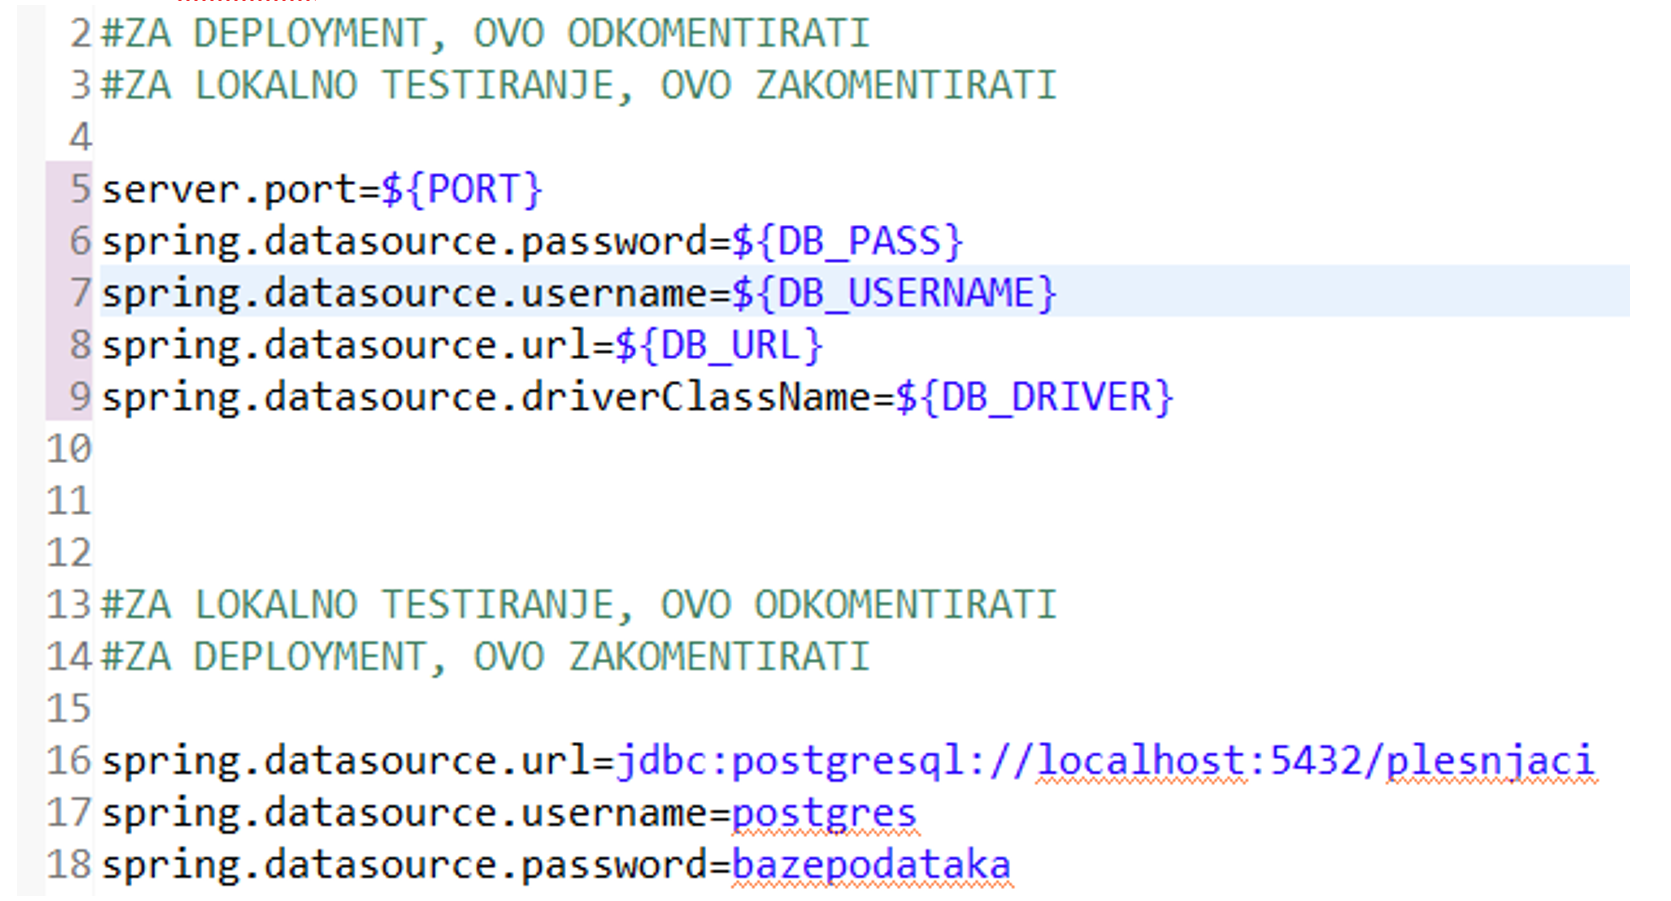
\includegraphics[width=\textwidth]{slike/deployment/slika2.png}
         	\caption{Kod datoteke application.properties}
         	\label{fig:my_label}
         \end{figure}
     
	     \begin{figure}[H]
	     	\centering
	     	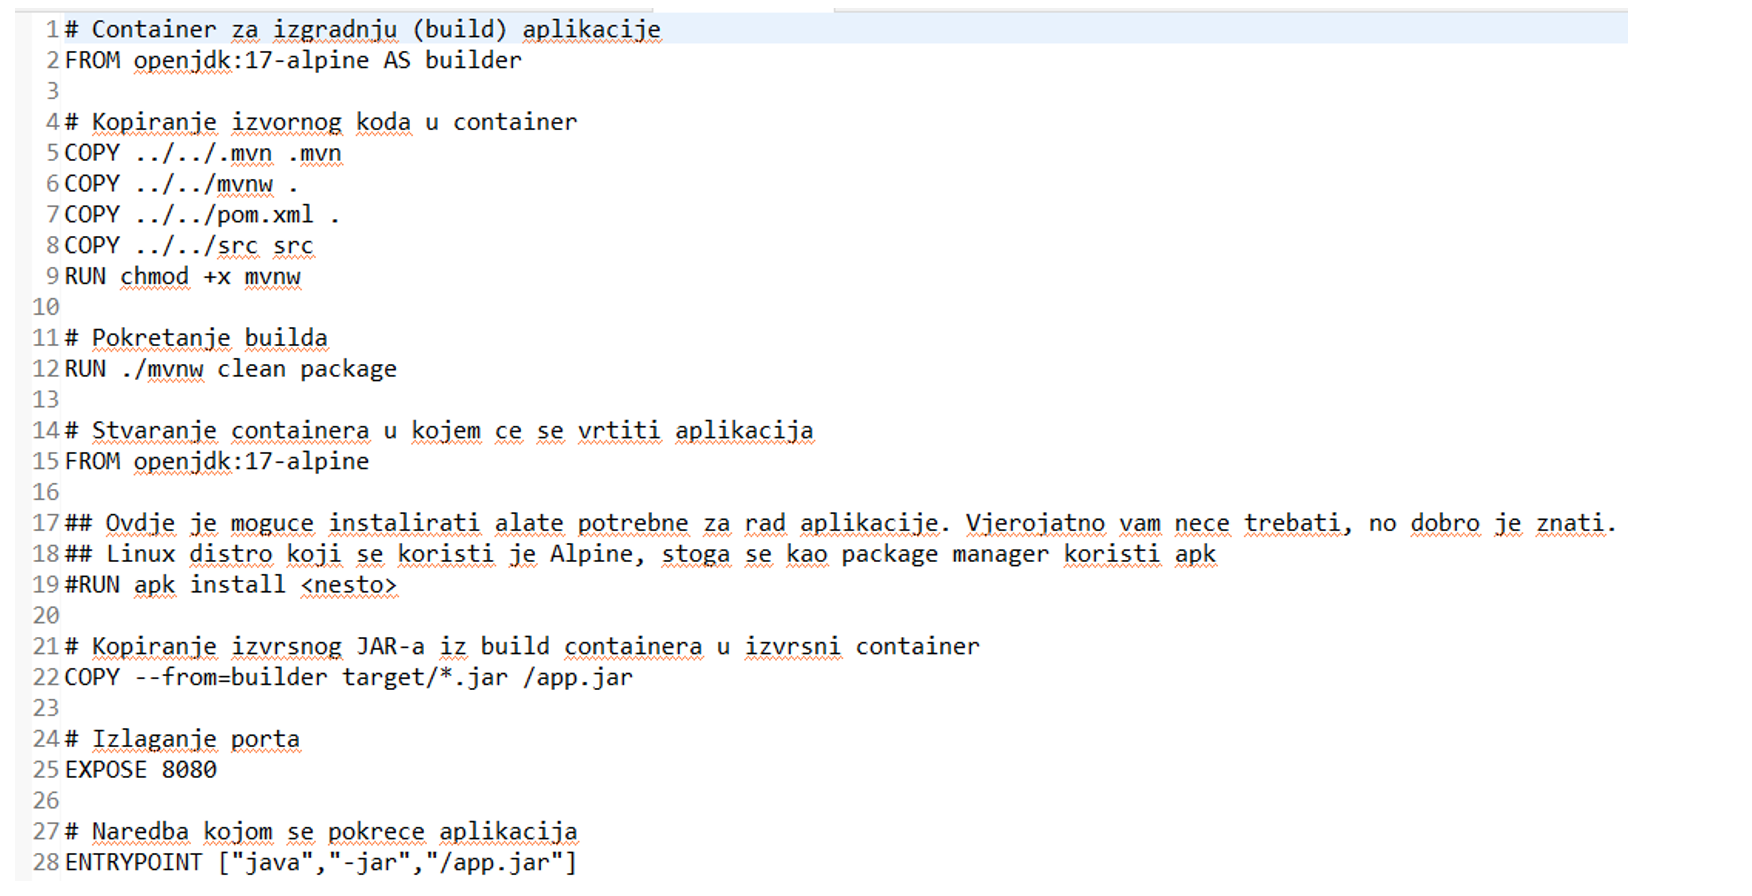
\includegraphics[width=\textwidth]{slike/deployment/slika3.png}
	     	\caption{Kod datoteke Dockerfile}
	     	\label{fig:my_label}
	     \end{figure}
     
        \textbf{\textit{Stvaranje backend aplikacije na Render-u}}\\

       	\textit{Na Render Dashboard-u treba kliknuti na „New“ pa odabrati „Web Service“ da bi se započelo stvaranje web aplikacije. Najprije je potrebno odabrati željeni GitLab repozitorij iz kojeg će se uzimati kod aplikacije klikom na tipku „Connect“ pored imena repozitorija. Na sljedećoj formi potrebno je u polje „Name“ upisati željeno ime aplikacije(ime će postati dio web adrese aplikacije), polje „Region“ treba postaviti na „Frankfurt“, polje „Branch“ postaviti na ime grane GitLab repozitorija s koje se uzima kod aplikacije, u polje „Root Directory“ treba upisati put do koda aplikacije u GitLab repozitoriju(npr. IzvorniKod/SpringBackend/Plesnjaci), postaviti polje „Environment“ na „Docker“ i konačno staviti „Instance Type“ na „Free“. Zatim treba stisnuti na gumb „Advanced“ da bi se otvorila dodatna forma. Na toj formi potrebno je dodati 5 envirnonment varijabli pomoću gumba „Add Environment Variable“ i nazvati ih identično onima na Slici 5.3. Vrijednost varijable „PORT“ su vrata na kojima radi baza podataka, „DB\_URL“ je URL baze podataka u formatu „jdbc:postgresql://hostname:port/database“, „DB\_USERNAME“ je ime vlasnika baze podataka, „DB\_PASS“ je lozinka vlasnika baze podataka, a „DB\_DRIVER“ treba postaviti na „org.postgresql.Driver“. Ukoliko je popunjeno polje „Root Directory“, polja „Docker Build Context Directory“ i „Dockerfile Path“ će imati „Root Directory“ kao prefiks(ako nije popunjeno prefiks se mora ručno dodati), a onda je u ta dva polja potrebno staviti „.“(za prvo) te „./docker/maven/Dockerfile“(za drugo). Ostala polja nije potrebno mijenjati ili popunjavati, a pritiskom na gumb „Create Web Service“ stvara se aplikacija. Novo stvorena aplikacija može se vidjeti na Render Dashboard-u gdje je dostupan i njezin URL.}
       	
       	\bigskip
       	\bigskip
       	
    \textbf{\textit{Priprema frontend aplikacije za puštanje u pogon}}\\
 
    \textit{U datoteci „package.json“ potrebno je u "dependencies" dodati dependancy za http-proxy-middleware, dotenv i express, u "scripts" treba dodati liniju "start-prod": "node app.js" te liniju "build": "react-scripts build" treba zamijeniti s "build": "yarn install \textnormal{\&\&} react-scripts build". Zatim treba dodati datoteku „setupProxy.js“ s kodom prikazanim na Slici 5.5 na putanju „./src/setupProxy.js“ te dodati datoteku „app.js“ s kodom prikazanim na Slici 5.6 na putanju „./app.js“.}
    \bigskip
		    \begin{figure}[H]
		    	\centering
		    	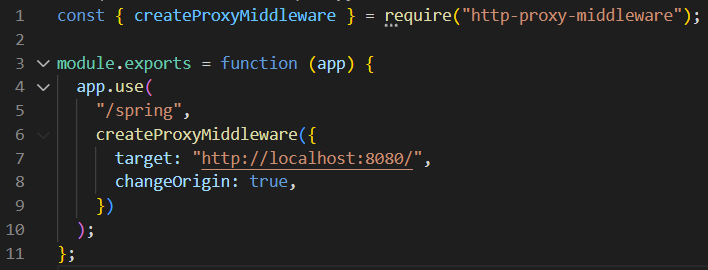
\includegraphics[width=\textwidth]{slike/deployment/slika4.png}
		    	\caption{Kod datoteke setupProxy.js}
		    	\label{fig:my_label}
		    \end{figure}
		
		 \begin{figure}[H]
			\centering
			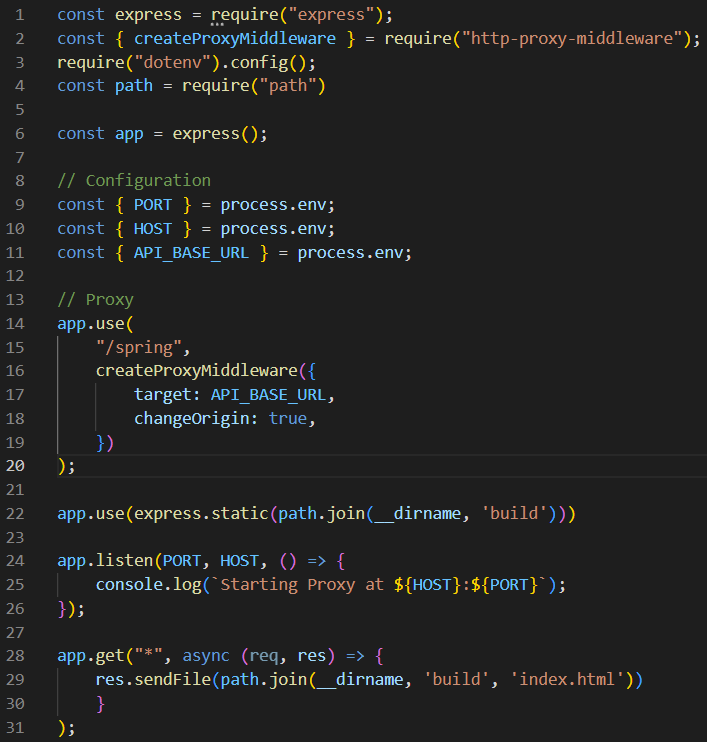
\includegraphics[width=\textwidth]{slike/deployment/slika5.png}
			\caption{Kod datoteke app.js}
			\label{fig:my_label}
		\end{figure}
	
	\newpage
	 \textbf{\textit{Stvaranje frontend aplikacije na Render-u}}\\
	\textit{Na Render Dashboard-u treba kliknuti na „New“ pa odabrati „Web Service“ da bi započelo stvaranje web aplikacije. Najprije je potrebno odabrati željeni GitLab repozitorij iz kojeg će se uzimati kod aplikacije klikom na tipku „Connect“ pored imena repozitorija. Na sljedećoj formi potrebno u polje „Name“ upisati željeno ime aplikacije(ime će postati dio web adrese aplikacije), polje „Region“ treba postaviti na „Frankfurt“, polje „Branch“ postaviti na ime grane GitLab repozitorija s koje se uzima kod aplikacije, u polje „Root Directory“ treba upisati put do koda aplikacije u GitLab repozitoriju(npr. IzvorniKod/ReactFrontend/plesnjaci) i postaviti polje „Envirotnment“ na „Node“. Zatim je potrebno polje „Build Command“ postaviti na „yarn build“ te polje „Start Command“ na „yarn start-prod“. Nakon toga treba stisnuti na gump „Advanced“ da bi se otvorila dodatna forma. Na toj formi potrebno je dodati jednu envirnonment varijablu pomoću gumba „Add Environment Variable“, nazvati ju „API\_BASE\_URL“ i postaviti njezinu vrijednost na URL backend aplikacije na Renderu koji je dostupan na Render Dashboard-u. Ostala polja nije potrebno mijenjati ili popunjavati, a pritiskom na gumb „Create Web Service“ stvara se aplikacija. Novo stvorena aplikacija može se vidjeti na Render Dashboard-u gdje je dostupan i njezin URL.}
	\bigskip
	
	 \textbf{\textit{Pokretanje aplikacije}}\\
	
	\textit{Aplikacija se pokreće upisivanjem linka https://plesnjaci-frontend.onrender.com u browser. Nakon dužeg perioda neaktivnosti aplikacija na Render-u će se automatski ugasiti te će se ponovno podignuti kada primi novi HTTP zahtjev bilo kakve vrste. U takvom slučaju je potrebno pričekati neko vrijeme(najviše nekoliko minuta) dok se aplikacija u potpunosti ne pokrene.}



    

 
	
		
		
	\chapter{Zaključak i budući rad}
		
	
		 \textit{Zadatak ove grupe bio je razvoj web aplikacije za organizaciju plesnjaka i tečajeva. Najvažnije stečeno znanje jest upravo rad u timu koji je došao sa raznim izazovima s kojima smo se morali snaći na najbolji mogući način. Voditelj grupe morao je koordinirati sedmero ljudi što nije bilo lako. U početku smo se susreli sa puno novih stvari koje je trebalo brzo naučiti i intenzivno raditi na aplikaciji i izradi dokumentacije. Učenje o alatima i novim tehnologijama koje su se koristile u izradi aplikacije i dokumentacije oduzimalo je puno vremena. Nakon međuispita bilo je ipak lakše jer smo se bolje  navikli na timski rad i  pomaganje jedni drugima.  Sigurni smo da bi aplikacija i više napredovala da smo kao tim imali više vremena, no uz fakultetske i ostale obaveze svakog člana tima zadovoljni smo sa konačnom aplikacijom. Komunikacija među članovima tima bila je kvalitetna.Komunicirali smo preko Whatsapp-a i Discorda. Održavali smo sastanke na kojima smo diskutirali što treba raditi, objašnjavali što je dosad napravljeno i dijelili nove zadatke. Sastanci su se održavali prema potrebi.  U konačnici, zaključili smo da su  opuštena atmosfera, pomaganje i organizirani voditelj ključne stvari za dobar krajnji rezultat. }
         
    
		\eject 
	\chapter*{Popis literature}
		\addcontentsline{toc}{chapter}{Popis literature}
	
		
		\begin{enumerate}
			
			
			\item  Programsko inženjerstvo, FER ZEMRIS, \url{http://www.fer.hr/predmet/proinz}
			
			\item  I. Sommerville, "Software engineering", 8th ed, Addison Wesley, 2007.
			
			\item  The Unified Modeling Language, \url{https://www.uml-diagrams.org/}
			
			\item  Astah Community, \url{http://astah.net/editions/uml-new}
			
			\item Jović, Frid, „UML zadaci za vjezbu" (moodle)
			
			\item Tehnička predavanja tvrtke Croz, \url{https://gitlab.com/progi-deploy-demo}
			
			\item React tutorial course, \url{https://www.w3schools.com/REACT/DEFAULT.ASP}
			
		\end{enumerate}
		
		 
	
	
	\begingroup
	\renewcommand*\listfigurename{Indeks slika i dijagrama}
	%\renewcommand*\listtablename{Indeks tablica}
	%\let\clearpage\relax
	\listoffigures
	%\vspace{10mm}
	%\listoftables
	\endgroup
	\addcontentsline{toc}{chapter}{Indeks slika i dijagrama}


	
	\eject 
		
	\chapter*{Dodatak: Prikaz aktivnosti grupe}
		\addcontentsline{toc}{chapter}{Dodatak: Prikaz aktivnosti grupe}
		
		\section*{Dnevnik sastajanja}
		
		\textbf{\textit{Kontinuirano osvježavanje}}\\
		
		 \textit{U ovom dijelu potrebno je redovito osvježavati dnevnik sastajanja prema predlošku.}
		
		\begin{packed_enum}
			\item  sastanak
			
			\item[] \begin{packed_item}
				\item Datum: 24. listopada 2022.
				\item Prisustvovali: M.Brlek, A.Cirkveni, M.Čukić, J.Gegač, V.Kežman, F.Šiktar, K.Žižić
				\item Teme sastanka:
				\begin{packed_item}
					\item  upoznavanje alata za pisanje dokumentacije
					\item  podjela poslova oko početne dokumentacije (opis, funkcionalni zahtjevi, dijagram obrazaca uporabi)
				\end{packed_item}
			\end{packed_item}
			
			\item  sastanak
			\item[] \begin{packed_item}
				\item Datum: 27. listopada 2022.
				\item Prisustvovali: M.Brlek, J.Gegač, F.Šiktar
				\item Teme sastanka:
				\begin{packed_item}
					\item  druga labaratorijska vježba, prokomentirali smo početnu dokumentaciju
				\end{packed_item}
			\end{packed_item}
		
			\item  sastanak
			\item[] \begin{packed_item}
				\item Datum: 31. listopada 2022.
				\item Prisustvovali: M.Brlek, F.Šiktar
				\item Teme sastanka:
				\begin{packed_item}
					\item  proučili poslove za nastavak pisanja dokumentacije
					\item  podijelili ekipi poslove (prepravak predhodne dokumentacije + razrada baze podataka)
				\end{packed_item}
			\end{packed_item}
			
			\item  sastanak
			\item[] \begin{packed_item}
				\item Datum: 1. studenog 2022.
				\item Prisustvovali: M.Brlek, A.Cirkveni, M.Čukić, J.Gegač, F.Šiktar, K.Žižić
				\item Teme sastanka:
				\begin{packed_item}
					\item  upoznavanje tima s modelom baze i njena dorada
					\item  razrada osnovnog izgleda web aplikacije
					\item  podijeljeni poslovi do sljedeće laboratorijske vjezbe
				\end{packed_item}
			\end{packed_item}
		
			\item  sastanak 
			\item[] \begin{packed_item}
				\item Datum: 3. studenog 2022.
				\item Prisustvovali: K.Žižić
				\item Teme sastanka:
				\begin{packed_item}
					\item treća laboratorijska vježba, prokomentirali smo ERD baze te Use Case dijagrame 
				\end{packed_item}
			\end{packed_item}
		
			\item  sastanak 
			\item[] \begin{packed_item}
				\item Datum: 12. studenog 2022.
				\item Prisustvovali: M.Brlek, A.Cirkveni
				\item Teme sastanka:
				\begin{packed_item}
					\item prezentiranje generičke stranice, pokazivanje kako se pokreće
					\item upute za rad u Reactu
					\item podijeljeni poslovi
				\end{packed_item}
			\end{packed_item}
		
			\item  sastanak 
			\item[] \begin{packed_item}
				\item Datum: 15. studenog 2022.
				\item Prisustvovali: M.Brlek, M.Čukić, J.Gegač, F.Šiktar, K.Žižić
				\item Teme sastanka:
				\begin{packed_item}
					\item prezentiranje generičke stranice, pokazivanje kako se pokrece
					\item diskutirana komunikacija između frontenda i backenda
					\item definirano što se očekuje od generičke funkcionalnosti
				\end{packed_item}
			\end{packed_item}
		
			\item  sastanak 
			\item[] \begin{packed_item}
				\item Datum: 21. prosinca 2022.
				\item Prisustvovali: A.Cirkveni, F.Šiktar
				\item Teme sastanka:
				\begin{packed_item}
					\item demonstracija alfa inačice
					\item definirani rokovi daljnjeg razvoja
				\end{packed_item}
			\end{packed_item}
		
			\item  sastanak 
			\item[] \begin{packed_item}
				\item Datum: 12. siječnja 2023.
				\item Prisustvovali: M.Brlek, F.Šiktar, K.Žižić
				\item Teme sastanka:
				\begin{packed_item}
					\item demonstracija gotove stranice
					\item prodiskutirana predaja projekta
				\end{packed_item}
			\end{packed_item}
			
			%
			
		\end{packed_enum}
		
		\eject
		\section*{Tablica aktivnosti}
		
			\textbf{\textit{Kontinuirano osvježavanje}}\\
			
			 \textit{Napomena: Doprinose u aktivnostima treba navesti u satima po članovima grupe po aktivnosti.}

			\begin{longtblr}[
					label=none,
				]{
					vlines,hlines,
					width = \textwidth,
					colspec={X[7, l]X[1, c]X[1, c]X[1, c]X[1, c]X[1, c]X[1, c]X[1, c]}, 
					vline{1} = {1}{text=\clap{}},
					hline{1} = {1}{text=\clap{}},
					rowhead = 1,
				} 
				\multicolumn{1}{c|}{} & \multicolumn{1}{c|}{\rotatebox{90}{\textbf{Marko Brlek}}} & \multicolumn{1}{c|}{\rotatebox{90}{\textbf{Andrej Cirkveni }}} &	\multicolumn{1}{c|}{\rotatebox{90}{\textbf{Martin Čukić }}} & \multicolumn{1}{c|}{\rotatebox{90}{\textbf{Josip Gegač }}} &	\multicolumn{1}{c|}{\rotatebox{90}{\textbf{Viktoria Kežman }}} & \multicolumn{1}{c|}{\rotatebox{90}{\textbf{Filip Šiktar }}} &	\multicolumn{1}{c|}{\rotatebox{90}{\textbf{Karlo Žižić }}} \\  
				Upravljanje projektom 		& 8 &  &  &  &  & 2 & 2\\ 
				Opis projektnog zadatka 	&  & 5&  &  & 4  &  & \\ 
				
				Funkcionalni zahtjevi       &  &  & 2 &  &  & 4 &  \\ 
				Opis pojedinih obrazaca 	&  & 2 &  &  7& 2 &  &  7\\ 
				Dijagram obrazaca 			&  &  & 3 &  3&  &  &  3\\ 
				Sekvencijski dijagrami 		&  & 2&  &  &  &  &  3\\ 
				Opis ostalih zahtjeva 		&  &  &  &  &  &  &  \\ 

				Arhitektura i dizajn sustava	 & 2 &  &  &  & 6  & 2 &  \\ 
				Baza podataka				& 6 &  &  &  &  & 6 &   \\ 
				Dijagram razreda 			&  &  &  &  & 4 &  &   \\ 
				Dijagram stanja				&  &  &  &  & 4  &  &  \\ 
				Dijagram aktivnosti 		&  &  &  &  & 3 &  &  \\ 
				Dijagram komponenti			&  &  &  &  &  2 &  &  \\ 
				Korištene tehnologije i alati 		&  &  &  &  & 2 &  &  \\ 
				Ispitivanje programskog rješenja 	&  &  &  &  &  &  &  \\ 
				Dijagram razmještaja			&  &  &  &  & 1 &  &  \\ 
				Upute za puštanje u pogon 		&  &  &  & 6 &  &  &  \\  
				Dnevnik sastajanja 			& 1 &  &  &  &  &  &  \\ 
				Zaključak i budući rad 		&  &  &  &  &  1 &  &  \\  
				Popis literature 			&  &  &  &  &  1&  &  \\  
				&  &  &  &  &  &  &  \\ \hline 
				Izrada login i register stranice 			& 6 & 5 &  &  & 9 &  &  \\ 
				Izrada baze podataka 				&  &  &  &  &  & 5 &  \\  
				Kreiranje login kontrolera na backendu		 			&  &  & 6 & 5 &  & 3 & 6\\  
				Puštanje aplikacije u pogon 			& 12 &  &  & 8 &  &  &  \\ 
				Dizajniranje stranice 				& 20 & 30 &  & 6 & 24 & 1 &  \\  
				Osposobljavanje admin funkcionalnosti 				& 6 & 3 &  &  &  & 3.5 & 3 \\  
				Upravljanje podacima klijenta 				& 20 & 15 &  &  &  & 15 & 15 \\  
				Upravljanje podacima kluba 				& 8 & 3 &  & 4 &  & 21 & 15 \\  
				Upravljanje podacima plesa 				& 4 &  &  &  &  & 5 & 15 \\  
				Upravljanje podacima plesnjaka 				& 13 &  &  &  &  & 17.5 & 12.5 \\  
				Upravljanje podacima tečaja 				& 22 &  &  &  &  & 10 & 6 \\ 
				Testiranje 				& 4 &  &  & 3 &  & 11.5 & 5 \\  
				 
			\end{longtblr}
					
					
		\eject
		\section*{Dijagrami pregleda promjena}
		
		
		\textit{Zbog puno grana i raznih spajanja izdvojeni su dijagrami promjena za grane master, develop i devdoc. }
		
			\begin{figure}[H]
			\centering
			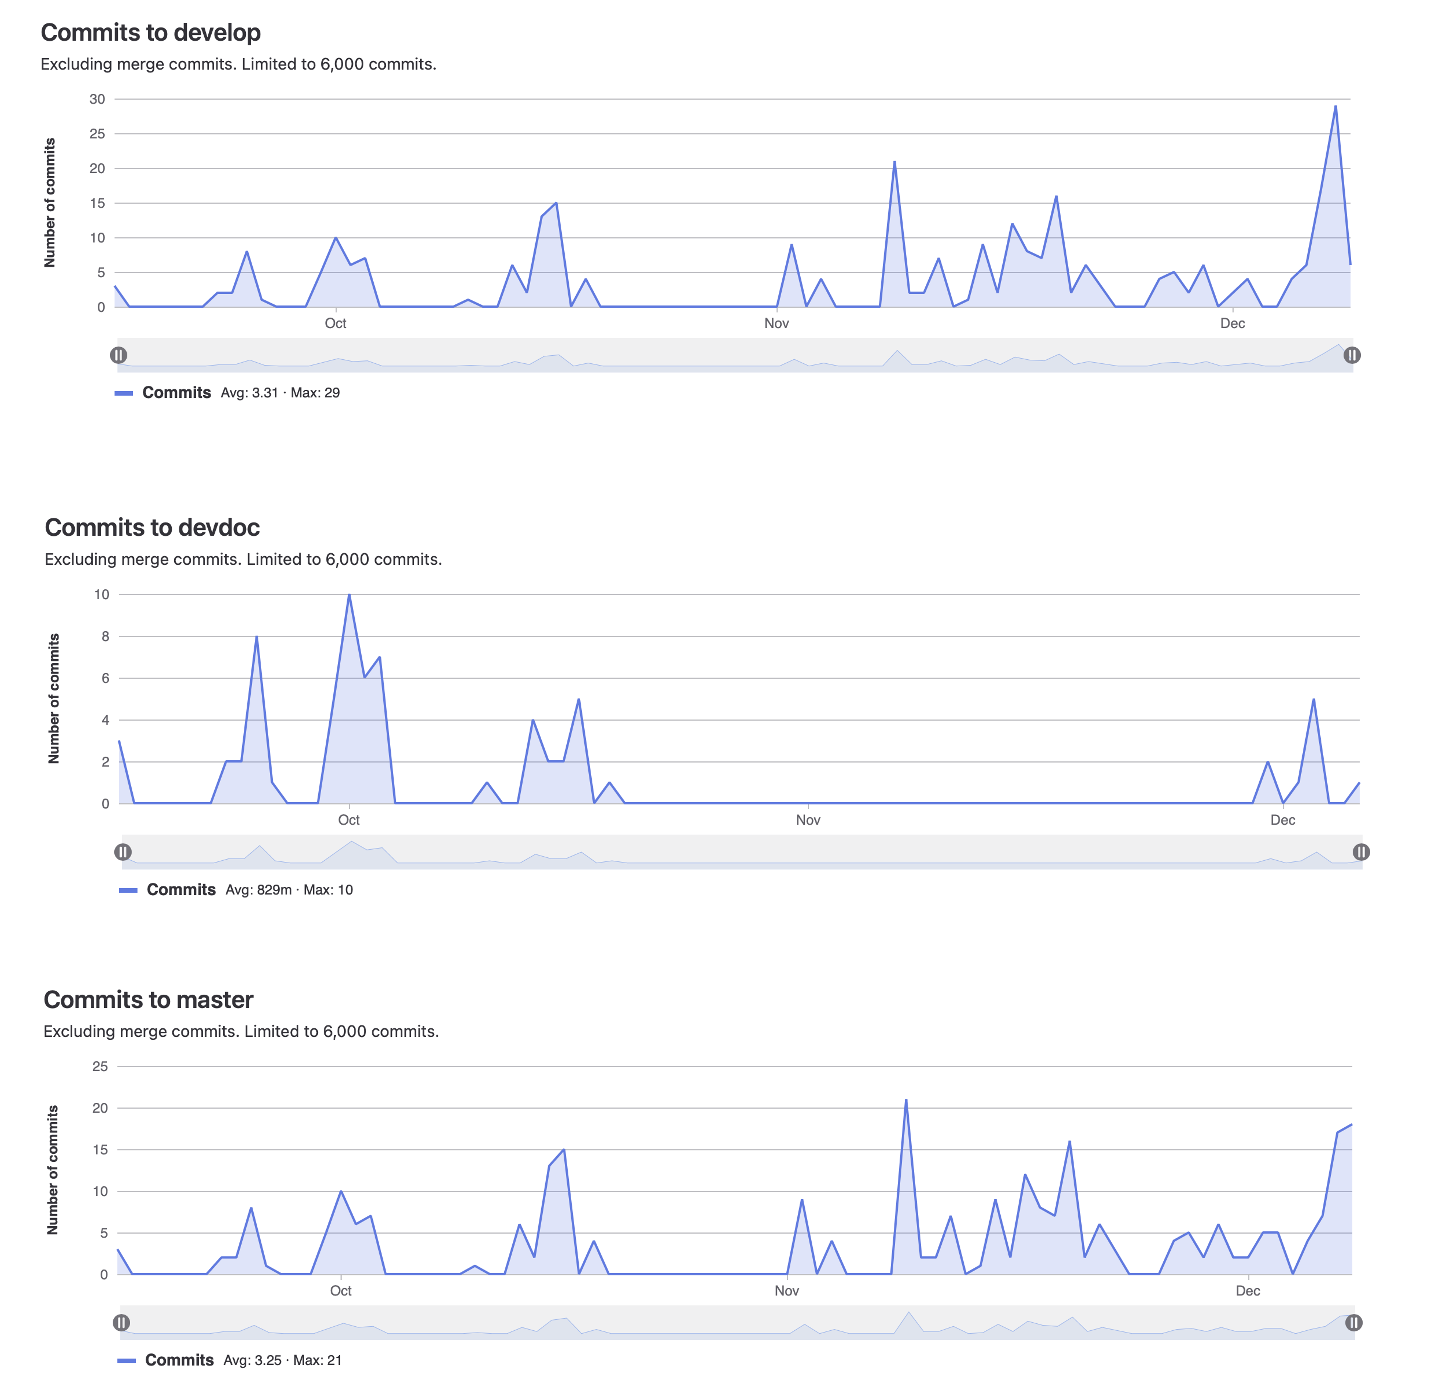
\includegraphics[width=\textwidth]{slike/dijagram_promjena.png}
			\caption{Dijagrami pregleda promjena nad datotekama izvornog koda i dokumentacije}
			\label{fig:my_label}
		\end{figure}
		
	


\end{document} %naredbe i tekst nakon ove naredbe ne ulaze u izgrađen dokument 


